% Options for packages loaded elsewhere
\PassOptionsToPackage{unicode}{hyperref}
\PassOptionsToPackage{hyphens}{url}
%
\documentclass[
]{book}
\usepackage{lmodern}
\usepackage{amssymb,amsmath}
\usepackage{ifxetex,ifluatex}
\ifnum 0\ifxetex 1\fi\ifluatex 1\fi=0 % if pdftex
  \usepackage[T1]{fontenc}
  \usepackage[utf8]{inputenc}
  \usepackage{textcomp} % provide euro and other symbols
\else % if luatex or xetex
  \usepackage{unicode-math}
  \defaultfontfeatures{Scale=MatchLowercase}
  \defaultfontfeatures[\rmfamily]{Ligatures=TeX,Scale=1}
\fi
% Use upquote if available, for straight quotes in verbatim environments
\IfFileExists{upquote.sty}{\usepackage{upquote}}{}
\IfFileExists{microtype.sty}{% use microtype if available
  \usepackage[]{microtype}
  \UseMicrotypeSet[protrusion]{basicmath} % disable protrusion for tt fonts
}{}
\makeatletter
\@ifundefined{KOMAClassName}{% if non-KOMA class
  \IfFileExists{parskip.sty}{%
    \usepackage{parskip}
  }{% else
    \setlength{\parindent}{0pt}
    \setlength{\parskip}{6pt plus 2pt minus 1pt}}
}{% if KOMA class
  \KOMAoptions{parskip=half}}
\makeatother
\usepackage{xcolor}
\IfFileExists{xurl.sty}{\usepackage{xurl}}{} % add URL line breaks if available
\IfFileExists{bookmark.sty}{\usepackage{bookmark}}{\usepackage{hyperref}}
\hypersetup{
  pdftitle={Estatística Aplicada à Pesquisa},
  pdfauthor={Agatha Rodrigues},
  hidelinks,
  pdfcreator={LaTeX via pandoc}}
\urlstyle{same} % disable monospaced font for URLs
\usepackage{color}
\usepackage{fancyvrb}
\newcommand{\VerbBar}{|}
\newcommand{\VERB}{\Verb[commandchars=\\\{\}]}
\DefineVerbatimEnvironment{Highlighting}{Verbatim}{commandchars=\\\{\}}
% Add ',fontsize=\small' for more characters per line
\usepackage{framed}
\definecolor{shadecolor}{RGB}{248,248,248}
\newenvironment{Shaded}{\begin{snugshade}}{\end{snugshade}}
\newcommand{\AlertTok}[1]{\textcolor[rgb]{0.94,0.16,0.16}{#1}}
\newcommand{\AnnotationTok}[1]{\textcolor[rgb]{0.56,0.35,0.01}{\textbf{\textit{#1}}}}
\newcommand{\AttributeTok}[1]{\textcolor[rgb]{0.77,0.63,0.00}{#1}}
\newcommand{\BaseNTok}[1]{\textcolor[rgb]{0.00,0.00,0.81}{#1}}
\newcommand{\BuiltInTok}[1]{#1}
\newcommand{\CharTok}[1]{\textcolor[rgb]{0.31,0.60,0.02}{#1}}
\newcommand{\CommentTok}[1]{\textcolor[rgb]{0.56,0.35,0.01}{\textit{#1}}}
\newcommand{\CommentVarTok}[1]{\textcolor[rgb]{0.56,0.35,0.01}{\textbf{\textit{#1}}}}
\newcommand{\ConstantTok}[1]{\textcolor[rgb]{0.00,0.00,0.00}{#1}}
\newcommand{\ControlFlowTok}[1]{\textcolor[rgb]{0.13,0.29,0.53}{\textbf{#1}}}
\newcommand{\DataTypeTok}[1]{\textcolor[rgb]{0.13,0.29,0.53}{#1}}
\newcommand{\DecValTok}[1]{\textcolor[rgb]{0.00,0.00,0.81}{#1}}
\newcommand{\DocumentationTok}[1]{\textcolor[rgb]{0.56,0.35,0.01}{\textbf{\textit{#1}}}}
\newcommand{\ErrorTok}[1]{\textcolor[rgb]{0.64,0.00,0.00}{\textbf{#1}}}
\newcommand{\ExtensionTok}[1]{#1}
\newcommand{\FloatTok}[1]{\textcolor[rgb]{0.00,0.00,0.81}{#1}}
\newcommand{\FunctionTok}[1]{\textcolor[rgb]{0.00,0.00,0.00}{#1}}
\newcommand{\ImportTok}[1]{#1}
\newcommand{\InformationTok}[1]{\textcolor[rgb]{0.56,0.35,0.01}{\textbf{\textit{#1}}}}
\newcommand{\KeywordTok}[1]{\textcolor[rgb]{0.13,0.29,0.53}{\textbf{#1}}}
\newcommand{\NormalTok}[1]{#1}
\newcommand{\OperatorTok}[1]{\textcolor[rgb]{0.81,0.36,0.00}{\textbf{#1}}}
\newcommand{\OtherTok}[1]{\textcolor[rgb]{0.56,0.35,0.01}{#1}}
\newcommand{\PreprocessorTok}[1]{\textcolor[rgb]{0.56,0.35,0.01}{\textit{#1}}}
\newcommand{\RegionMarkerTok}[1]{#1}
\newcommand{\SpecialCharTok}[1]{\textcolor[rgb]{0.00,0.00,0.00}{#1}}
\newcommand{\SpecialStringTok}[1]{\textcolor[rgb]{0.31,0.60,0.02}{#1}}
\newcommand{\StringTok}[1]{\textcolor[rgb]{0.31,0.60,0.02}{#1}}
\newcommand{\VariableTok}[1]{\textcolor[rgb]{0.00,0.00,0.00}{#1}}
\newcommand{\VerbatimStringTok}[1]{\textcolor[rgb]{0.31,0.60,0.02}{#1}}
\newcommand{\WarningTok}[1]{\textcolor[rgb]{0.56,0.35,0.01}{\textbf{\textit{#1}}}}
\usepackage{longtable,booktabs}
% Correct order of tables after \paragraph or \subparagraph
\usepackage{etoolbox}
\makeatletter
\patchcmd\longtable{\par}{\if@noskipsec\mbox{}\fi\par}{}{}
\makeatother
% Allow footnotes in longtable head/foot
\IfFileExists{footnotehyper.sty}{\usepackage{footnotehyper}}{\usepackage{footnote}}
\makesavenoteenv{longtable}
\usepackage{graphicx,grffile}
\makeatletter
\def\maxwidth{\ifdim\Gin@nat@width>\linewidth\linewidth\else\Gin@nat@width\fi}
\def\maxheight{\ifdim\Gin@nat@height>\textheight\textheight\else\Gin@nat@height\fi}
\makeatother
% Scale images if necessary, so that they will not overflow the page
% margins by default, and it is still possible to overwrite the defaults
% using explicit options in \includegraphics[width, height, ...]{}
\setkeys{Gin}{width=\maxwidth,height=\maxheight,keepaspectratio}
% Set default figure placement to htbp
\makeatletter
\def\fps@figure{htbp}
\makeatother
\setlength{\emergencystretch}{3em} % prevent overfull lines
\providecommand{\tightlist}{%
  \setlength{\itemsep}{0pt}\setlength{\parskip}{0pt}}
\setcounter{secnumdepth}{5}
\usepackage{booktabs}
\usepackage[]{natbib}
\bibliographystyle{apalike}

\title{Estatística Aplicada à Pesquisa}
\author{Agatha Rodrigues}
\date{2020-11-11}

\begin{document}
\maketitle

{
\setcounter{tocdepth}{1}
\tableofcontents
}
\hypertarget{sobre-esse-livro}{%
\chapter{Sobre esse livro}\label{sobre-esse-livro}}

Este livro tem como objetivo abordar todas as etapas de uma análise de dados, discutindo os tópicos do ponto de vista teórico e prático, utilizando o softaware \href{https://cran.r-project.org/}{R} como ferramenta de análise de dados.

Na versão atual, a parte teórica do livro está bastante resumida. Para aquele leitor que tenha interesse em aprofundar mais nos assuntos aqui abordados, recomendamos os livros \citet{morettin2020introduccaoa}, \citet{bussab2004estatistica} e \citet{magalhaes2002noccoes}.

Este material está em construção e em revisão aberta. Fique à vontade para corrigir qualquer tipo de erro que encontrar no nosso material.

\hypertarget{sobre-mim}{%
\section{Sobre mim}\label{sobre-mim}}

Eu sou doutora em Estatística pelo Instituto de Matemática e Estatística da Universidade de São Paulo (2018), com graduação em Estatística pela Universidade Federal de São Carlos (2010) e mestrado em Estatística pelo Instituto de Matemática e Estatística da Universidade de São Paulo (2013). Minhas áreas de pesquisa são: Análise de Confiabilidade, Análise de Sobrevivência e Bioestatística.

Tenho experiência em mais de 10 anos com pesquisa em Estatística aplicada à área da saúde, com atuações em hospitais oncológicos, departamentos de Obstetrícia e Ginecologia, Psiquiatria e também Psicologia. Já ministrei cursos de Estatística na pós-graduação do Departamento de Ginecologia e Obstetrícia da USP, trazendo uma abordagem de aulas teóricas e práticas em algum programa de análise de dados.

Atualmente sou docente no Departamento de Estatística da Universidade Federal do Espírito Santo (UFES), coordenadora do projeto de extensão ensinaR (que visa a divulgação, ensino e treinamento da comunidade sobre o software R) e cofundadora da R-Ladies Capítulo Vitória (\url{https://www.meetup.com/pt-BR/rladies-vitoria/} e \url{https://github.com/rladies/meetup-presentations_vitoria}).

Também sou a coordenadora do laboratório de Ciência de Dados da UFES, o DaSLab (\url{https://daslab-ufes.github.io/}) e do projeto de pesquisa certificado no CNPq: Ciência de Dados e Aprendizado Estatístico Aplicados à Saúde (\url{http://dgp.cnpq.br/dgp/espelhogrupo/2755579833615592}).

\begin{itemize}
\tightlist
\item
  Currículo lattes: \url{http://lattes.cnpq.br/3445977720574534}
\item
  GitHub: \url{https://github.com/agathasr}
\item
  Linkedin: \url{https://www.linkedin.com/in/agatha-rodrigues-0a8a6214a}
\item
  Email: \href{mailto:agatha.srodrigues@gmail.com}{\nolinkurl{agatha.srodrigues@gmail.com}}
\end{itemize}

\hypertarget{intro}{%
\chapter{Introdução}\label{intro}}

A Estatística é a ciência que engloba métodos para coleta, organização, descrição, análise e interpretação de dados, sendo estes estruturados (as estruturas usuais de bases de dados) ou não estruturados (como arquivos de textos, páginas da web, emails, midias sociais etc). Assim, podemos dizer que por meio da Estatística transformamos dados em informações para o auxílio de tomadas de decisões em situações de incerteza.

Devido à alta capacidade de armazenamento das mídias e ao uso generalizado de computadores, muitos dados estão sendo coletados e o mundo depende cada vez mais de dados para criar conhecimento, obter informações relevantes e prever melhor o futuro. No seu livro Homo Deus, de 2016, Yuval Noah Harari argumenta que todos as estruturas políticas e sociais podem ser vistas como sistemas de processamento de dados e que daí surge a religião Dataísmo: ``O Dataísmo declara que o universo consiste em fluxos de dados e que o valor de qualquer fenômeno ou entidade é determinada pela contribuição que dá para o processamento de dados'' (\url{https://pt.wikipedia.org/wiki/Dataísmo}).

Na pesquisa médica, em especial, são realizados estudos experimentais ou observacionais, levando à coleção de dados e o objetivo da investigação é responder a uma questão científica. Para exemplificar esse ponto, vamos considerar um problema da área da medicina obstétrica que consiste no estudo da idade gestacional do parto em gestações gemelares (de gêmeos).

A importância de se estudar a idade gestacional do parto em gestação gemelares se deve pelo elevado risco de prematuridade (parto antes de 37 semanas) em gestações múltiplas. Entre as mulheres com gestação gemelar, o parto prematuro que ocorre antes das 37 semanas é observado em mais de 50\% dos casos e quase 12\% antes de 32 semanas completas de gestação \citep{silva1995prematuridade}. Devido a este fato, observa-se uma taxa de mortalidade neonatal nas gestações gemelares de 6,4 vezes maior que nas gestações únicas (único feto) e essa taxa se mantém inalterada desde o ano de 2000 \citep{into2009child}.

O trabalho de parto é consequência de eventos fisiológicos, como por exemplo, o predomínio da ação estrogênica em relação à progesterônica. A progesterona é um hormônio fundamental para a manutenção da gravidez, e um declínio na ação da progesterona é fundamental para o início do parto na maioria das espécies de mamíferos, incluindo os primatas \citep{astle2003involvement}. A progesterona está presente na natureza, em humanos e animais (ovários, placenta, testículos e adrenal). Os seus percursores estão presentes nos vegetais, como a soja e o inhame, e constituem a principal fonte de produção da progesterona natural comercializada \citep{de2016prenatal}.

Em gestações com colo curto, também com risco de prematuridade, o uso de progesterona comercializada é um tratamento conhecido na literatura para diminuir o risco de prematuridade. No projeto liderado pela obstetra e profa. Dra. Maria de Lourdes Brizot (\url{http://lattes.cnpq.br/6273300603065618}), a pergunta que se deseja responder é:

\begin{quote}
O uso de progesterona diminui o risco de prematuridade em gestações gemelares?
\end{quote}

Para responder a essa pergunta, foi realizado um estudo prospectivo, randomizado, duplo
ensaio cego controlado por placebo que envolveu 390
gestações gemelares sem histórico de parto prematuro. Mulheres com gestações gemelares entre 18 e 21 semanas e 6 dias de gestação foram designadas aleatoriamente em um de dois grupos:

\begin{itemize}
\item
  \textbf{Tratamento com progesterona} - progesterona vaginal diária (200 mg) até 34 semanas e 6 dias de gestação (ou até o parto se este ocorreu antes de 35 semanas).
\item
  \textbf{Tratamento placebo} - óvulos de placebo até 34 semanas e 6 dias de gestação (ou até o parto se este ocorreu antes de 35 semanas).
\end{itemize}

Um comentário importante: placebo é toda e qualquer substância sem propriedades farmacológicas, administrada a pessoas ou grupo de pessoas como se tivesse propriedades terapêuticas. A palavra placebo vem do latim placere, que significa ``agradar''. Não entraremos em detalhes nesse material sobre tipos de estudo. Para este assunto e maiores discussões sobre placebo, recomendamos ver os slides ``Tipos de estudos'' disponível em \url{https://daslab-ufes.github.io/materiais/}.

Voltando ao problema da progesterona, houve 6 perdas de segmento no grupo progesterona e 4 perdas de segmento no grupo placebo, resultando em \(n=189\) no grupo progesterona e \(n=191\) no grupo placebo.

A variação nos dados faz com que a resposta não seja óbvia. Precisamos de ferramentas estatísticas para determinar se a
diferença é tão grande que devemos rejeitar a noção de que foi devido ao acaso.
No caso do estudo da progesterona, a diferença na proporção
de prematuridade do grupo progesterona e do grupo controle é
devido à flutuações aleatórias ou é um indício de que o uso de progesterona é um protocolo mais eficiente?

A seguir são apresentadas as bases de dados que consideramos no decorrer desse material.

\hypertarget{bases-de-dados}{%
\section{Bases de dados}\label{bases-de-dados}}

\hypertarget{dados_gemelares}{%
\subsection{Gestações gemelares}\label{dados_gemelares}}

A base de dados fictícia de gestações gemelares é baseada no estudo citado anteriormente sobre o efeito do uso de progesterona em gestações gemelares. Sabe-se que os históricos obstétrico e clínico da gestante e informações da gestação também podem influenciar a idade gestacional do parto e, por esse motivo, também foram avaliados. São as características observadas:

\begin{figure}
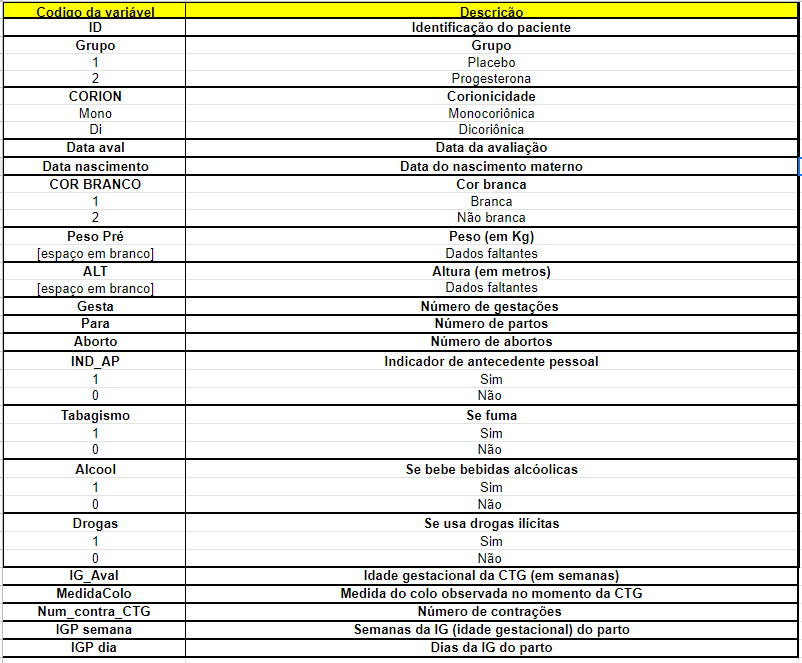
\includegraphics[width=1\linewidth]{figures/dicionario_dados_progest} \caption{Variáveis da base de dados gestações gemelares.}\label{fig:dic1}
\end{figure}

A seguir está o exemplo de como os dados de 5 indivíduos estão tabulados.

\begin{tabular}{r|r|l|l|l|r|l|l|r|r|r|r|r|r|r|r|r|r|r|r|l}
\hline
ID & Grupo & CORION & Data aval & Data nascimento & COR BRANCO & Peso Pré & ALT & Gesta & Para & Aborto & IND\_AP & Tabagismo & Alcool & Drogas & IG\_Aval & MedidaColo & Num\_contra\_CTG & IGP semana & IGP dia & oi\\
\hline
18 & 2 & Di & 2016-03-21 & 1987-03-29 & 1 & 80.0 & 1.59 & 1 & 0 & 0 & 1 & 0 & 0 & 0 & 31.43 & 20.00 & 7 & 37 & 5 & NA\\
\hline
19 & 2 & Di & 2016-02-17 & 1980-02-26 & 1 & NA & 1.62 & 4 & 3 & 0 & 0 & 1 & 1 & 0 & 27.00 & 6.60 & 2 & 33 & 2 & NA\\
\hline
20 & 1 & Di & 2017-12-14 & 1998-12-19 & 2 & 61.0 & 1.64 & 1 & 0 & 0 & 0 & 0 & 0 & 0 & 33.71 & 7.00 & 10 & 35 & 3 & NA\\
\hline
21 & 1 & Mono & 2017-04-23 & 1988-04-30 & 1 & 44.0 & 1.64 & 1 & 0 & 0 & 0 & 0 & 0 & 0 & 83.86 & 5.83 & 8 & 36 & 3 & NA\\
\hline
22 & 2 & Di & 2016-03-21 & 1995-03-27 & 2 & 100.0 & 1.59 & 2 & 1 & 0 & 1 & 0 & 1 & 0 & 33.71 & 12.10 & 3 & 37 & 6 & NA\\
\hline
\end{tabular}

Essa base de dados está disponível em \url{https://daslab-ufes.github.io/materiais/}, chamado de ``Dados gemelares''.

\hypertarget{gestauxe7uxf5es-gemelares---depressuxe3o-e-amamentauxe7uxe3o}{%
\subsection{Gestações gemelares - depressão e amamentação}\label{gestauxe7uxf5es-gemelares---depressuxe3o-e-amamentauxe7uxe3o}}

Esta base de dados fictícia apresenta informações sobre depressão e amamentação das mesmas observações consideradas na base de dados Gestações gemelares, apresentada no item anterior.

O questionário de depressão EDPS foi respondido pelas gestantes no primeiro trimestre gestacional e respondido novamente pelas mesmas gestantes no quarto mês pós-parto. Esse questionário retorna um escore (de 0 a 30 pontos), em que quanto maior seu valor, maior indicador de depressão.

Sobre a amamentação, foram divididos três grupos a depender das orientações sobre a amamentação recebidas durante o pré-natal. O grupo 1 é formado pelas gestantes que tiveram mentorias durante o pré-natal e acompanhamento nas amamentações das primeiras semanas; o grupo 2 é formado pelas gestações que receberam apenas orientações durante o pré-natal e no grupo 3 estão as gestantes que não receberam orientações sobre amamentação.

São as características observadas:

\begin{figure}
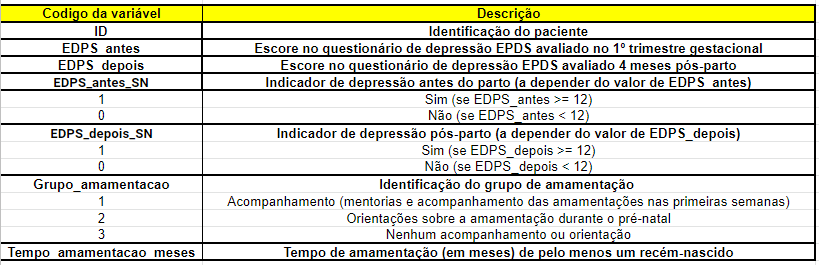
\includegraphics[width=1\linewidth]{figures/dicionario_dados_progest2} \caption{Variáveis da base de dados gestações gemelares - depressão e amamentação.}\label{fig:dic2}
\end{figure}

A seguir está o exemplo de como os dados de 5 indivíduos estão tabulados.

\begin{tabular}{r|r|r|r|r|r|r}
\hline
ID & EPDS\_antes & EPDS\_depois & EDPS\_antes\_SN & EDPS\_depois\_SN & Grupo\_amamentacao & Tempo\_amamentacao\_meses\\
\hline
18 & 2 & 1 & 0 & 0 & 1 & 10\\
\hline
19 & 6 & 3 & 0 & 0 & 2 & 4\\
\hline
20 & 10 & 8 & 0 & 0 & 2 & 15\\
\hline
21 & 15 & 18 & 1 & 1 & 2 & 11\\
\hline
22 & 3 & 4 & 0 & 0 & 2 & 8\\
\hline
\end{tabular}

Essa base de dados está disponível em \url{https://daslab-ufes.github.io/materiais/}, chamado de ``Dados gemelares - depressão e amamentação''.

\hypertarget{sobre-o-software-r}{%
\section{Sobre o software R}\label{sobre-o-software-r}}

R é um ambiente computacional e uma linguagem de programação para manipulação, análise e visualização de dados. É considerado um dos melhores ambiente computacional para essa finalidade. O R é mantido pela \href{https://cran.r-project.org/}{R Development Core Team} e está disponível para diferentes sistemas operacionais: Linux, Mac e Windows.

O software é livre, ou seja, gratuito, com código aberto em uma linguagem acessível. Nele estão implementadas muitas metodologias estatísticas. Muitas destas fazem parte do ambiente base de R e outras acompanham o ambiente sob a forma de pacotes, o que torna o R altamente expansível. Os pacotes são bibliotecas com dados e funções para diferentes áreas do conhecimento relacionado a estatística e áreas afins, devidamente documentados.

O R possui uma comunidade extremamente ativa, engajada desde o aprimoramento de ferramentas e desenvolvimento de novas bibliotecas, até o suporte aos usuários. Sobre o desenvolvimento de novas bibliotecas, um pesquisador em Estatística que desenvolve um novo modelo estatístico pode disponibilizar o seu modelo em um pacote acessível a que se interessam pelo modelo.

Além disso, a disponibilidade e compartilhamento da pesquisa em um pacote no R é uma boa prática quando falamos de reprodutibilidade na Ciência. Ainda nesse ponto, realizar as análises de uma pesquisa aplicada em um programa livre e acessível a todos é um dos principais pontos para permitir reprodutibilidade.

Ao optar por programar em R também implica na escolha de uma IDE (Integrated Development Environment) que, na grande maioria dos casos, será o \href{https://rstudio.com}{RStudio}. O RStudio é um conjunto de ferramentas integradas projetadas para editar e executar os códigos em R. Assim, quando for o interesse utilizar o R, só precisa abrir o RStudio (R é automaticamente carregado).

Para instalação do R e do RStudio, veja a Seção que segue.

\hypertarget{instalauxe7uxe3o-r-e-rstudio}{%
\section{Instalação R e RStudio}\label{instalauxe7uxe3o-r-e-rstudio}}

\hypertarget{instalauxe7uxe3o-r}{%
\subsection{Instalação R}\label{instalauxe7uxe3o-r}}

Nessa Seção, vamos apresentar como instalar o R e o RStudio para os três sistemas operacionais: Windows, MAC e Linux, respectivamente.

\hypertarget{para-windows}{%
\subsubsection{Para Windows}\label{para-windows}}

Os passos para instalar o R quando o sistema operacional é Windows são os seguintes:

\begin{enumerate}
\def\labelenumi{\arabic{enumi})}
\tightlist
\item
  Entre neste \href{https://cran.r-project.org/bin/windows/base/}{link} para acessar a página do R e clique em Download, como no link destacado em retângulo vermelho na Figura \ref{fig:windows1}. Note que o 3.6.1 é o número da versão mais recente disponível no momento da construção desse material (5/7/19).
\end{enumerate}

\begin{figure}
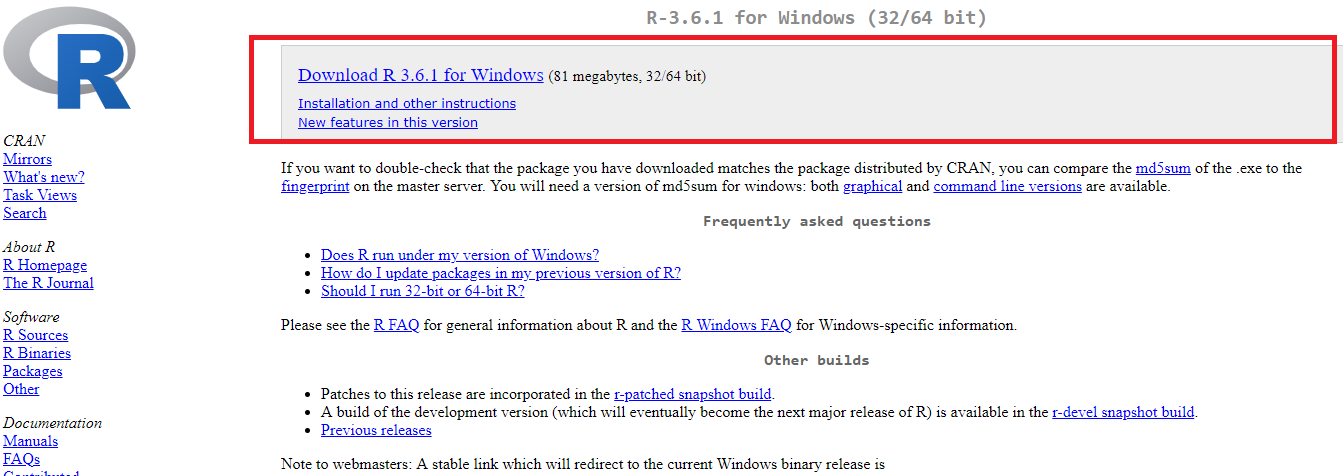
\includegraphics[width=1\linewidth]{figures/install_Windows} \caption{Download R para Windows}\label{fig:windows1}
\end{figure}

\begin{enumerate}
\def\labelenumi{\arabic{enumi})}
\setcounter{enumi}{1}
\tightlist
\item
  Salve o arquivo de instalação em algum caminho de interesse do seu computador. Por exemplo, na Figura \ref{fig:windows2} mostra que a pasta é ``Downloads''.
\end{enumerate}

\begin{figure}
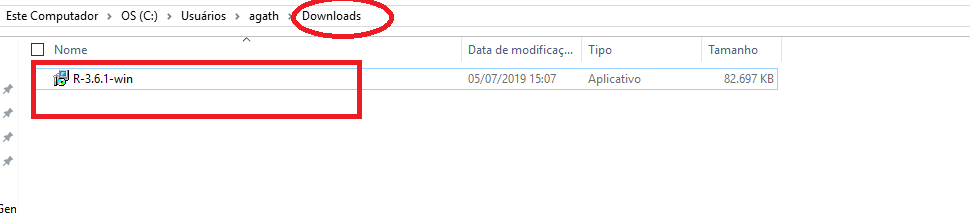
\includegraphics[width=1\linewidth]{figures/install_Windows2} \caption{Instalador}\label{fig:windows2}
\end{figure}

\begin{enumerate}
\def\labelenumi{\arabic{enumi})}
\setcounter{enumi}{2}
\tightlist
\item
  Clique duas vezes com o botão esquerdo no instalador para iniciar a instalação. O próximo passo é escolher a lingua para instalação. Na Figura \ref{fig:windows3} abaixo é português.
\end{enumerate}

\begin{figure}
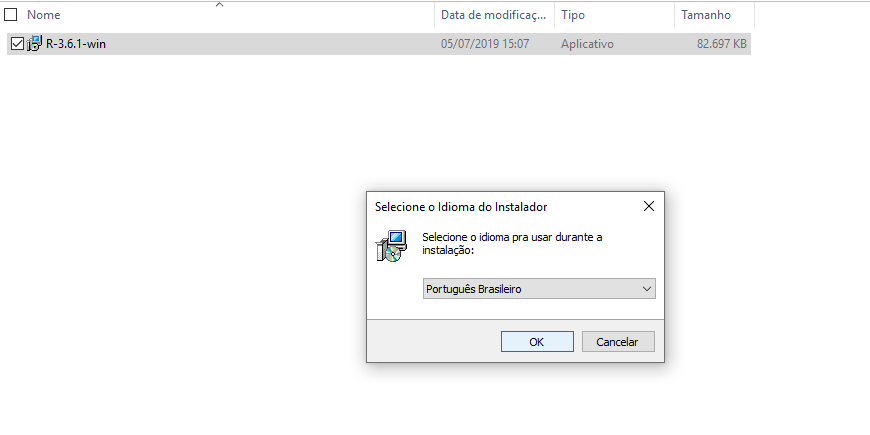
\includegraphics[width=1\linewidth]{figures/install_Windows3} \caption{Escolha da lingua para instalação}\label{fig:windows3}
\end{figure}

\begin{enumerate}
\def\labelenumi{\arabic{enumi})}
\setcounter{enumi}{3}
\tightlist
\item
  Clique em ``Próximo'' nas próximas janelas, como nas Figuras \ref{fig:windows4} a \ref{fig:windows9}.
\end{enumerate}

\begin{figure}
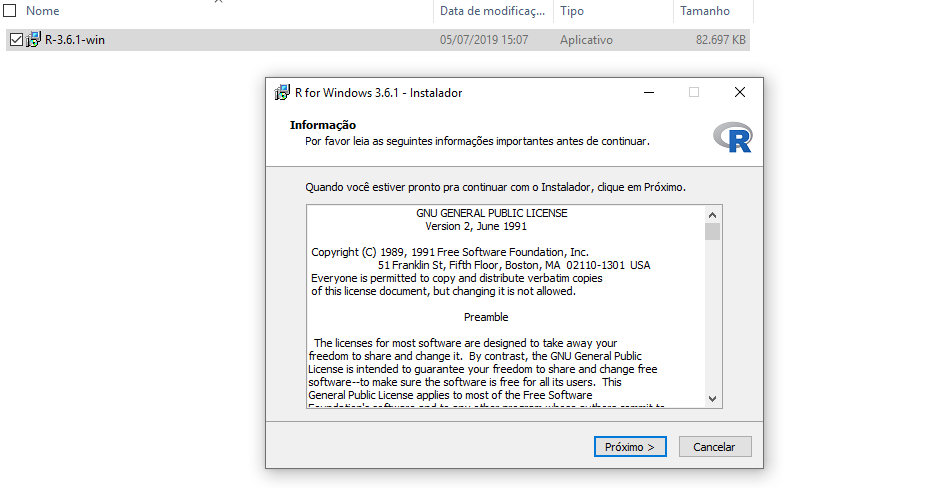
\includegraphics[width=1\linewidth]{figures/install_Windows4} \caption{Próximo }\label{fig:windows4}
\end{figure}

\begin{figure}
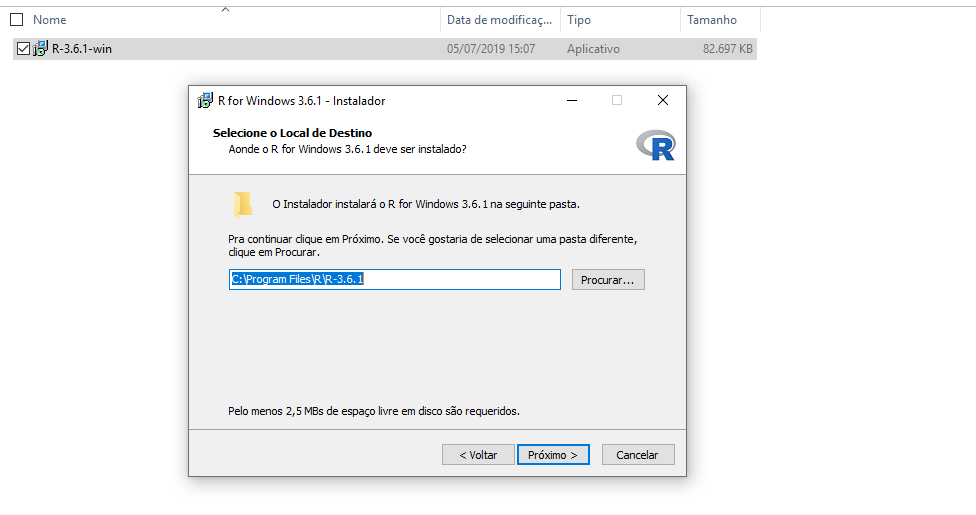
\includegraphics[width=1\linewidth]{figures/install_Windows5} \caption{\label{fig:windows5}Próximo }\label{fig:windows5}
\end{figure}

\begin{figure}
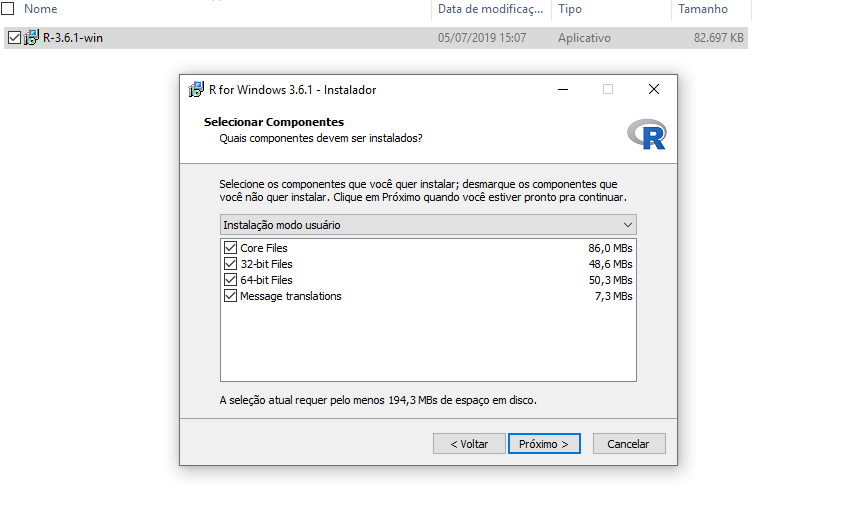
\includegraphics[width=1\linewidth]{figures/install_Windows6} \caption{\label{fig:windows6}Próximo }\label{fig:windows6}
\end{figure}

\begin{figure}
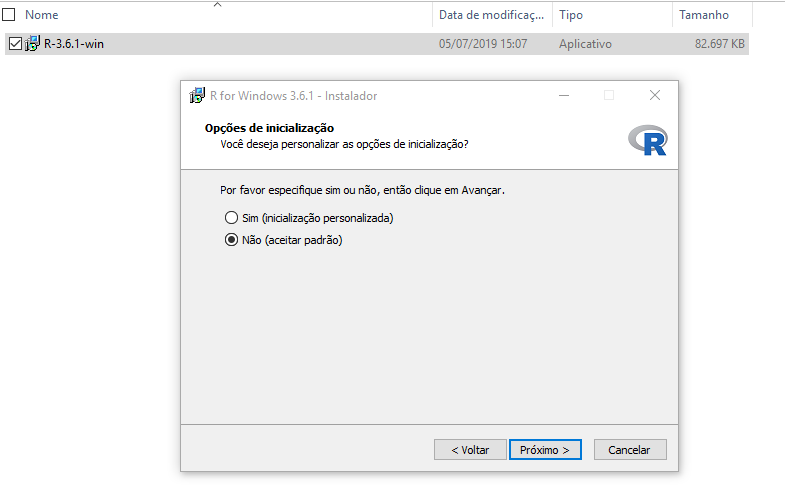
\includegraphics[width=1\linewidth]{figures/install_Windows7} \caption{\label{fig:windows7}Próximo }\label{fig:windows7}
\end{figure}

\begin{figure}
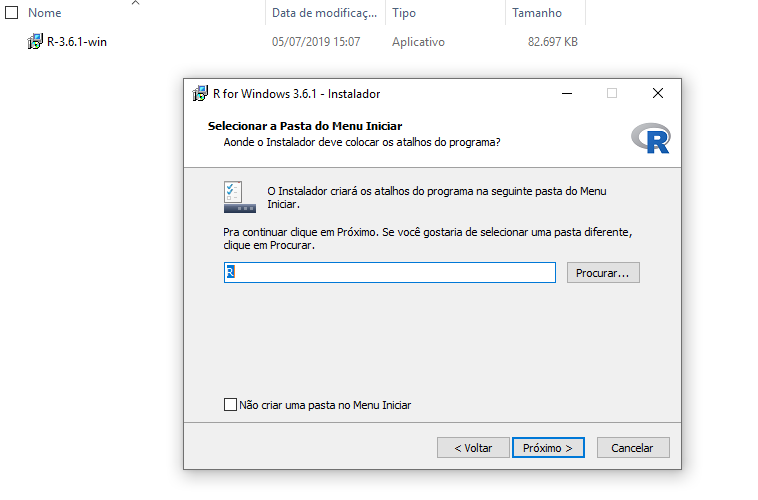
\includegraphics[width=1\linewidth]{figures/install_Windows8} \caption{\label{fig:windows8}Próximo }\label{fig:windows8}
\end{figure}

\begin{figure}
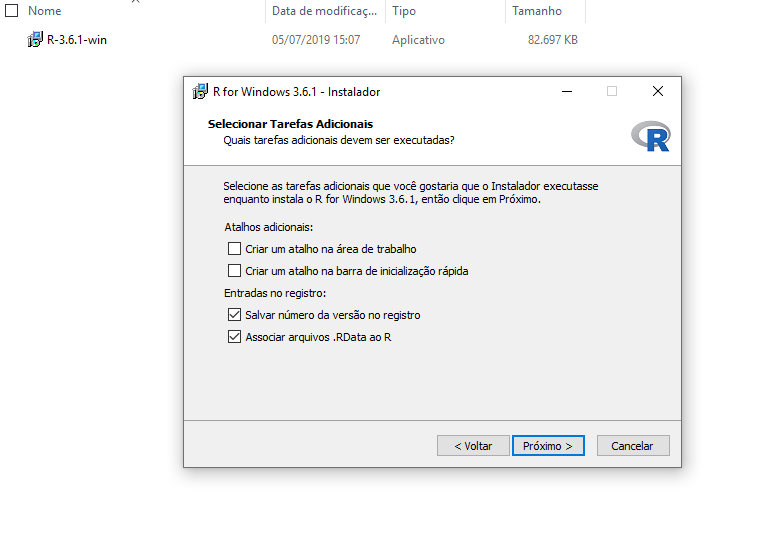
\includegraphics[width=1\linewidth]{figures/install_Windows9} \caption{\label{fig:windows9}Próximo }\label{fig:windows9}
\end{figure}

\begin{enumerate}
\def\labelenumi{\arabic{enumi})}
\setcounter{enumi}{4}
\tightlist
\item
  Pronto, agora o software R será instalado, como na Figura \ref{fig:windows10}, e quando terminar, aparecerá uma janela como apresentado na Figura \ref{fig:windows11}.
\end{enumerate}

\begin{figure}
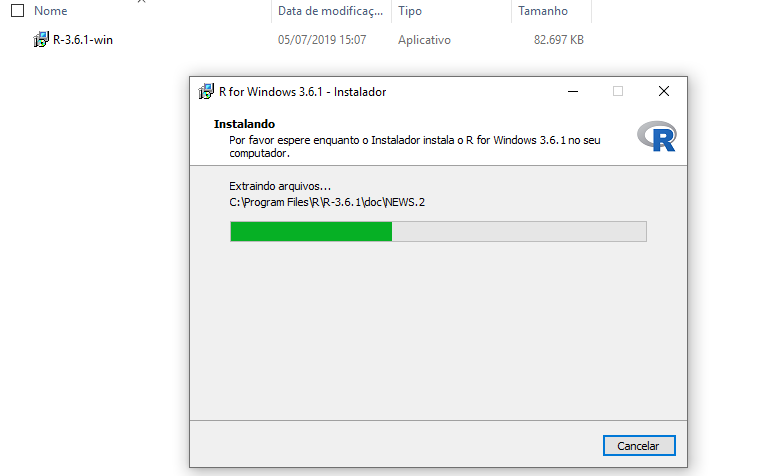
\includegraphics[width=1\linewidth]{figures/install_Windows10} \caption{\label{fig:windows10}Instalação do R}\label{fig:windows10}
\end{figure}

\begin{figure}
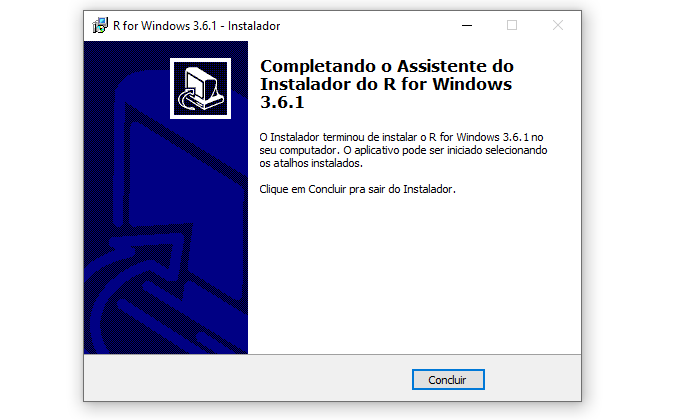
\includegraphics[width=1\linewidth]{figures/install_Windows11} \caption{\label{fig:windows11}Pronto: R instalado}\label{fig:windows11}
\end{figure}

\hypertarget{para-mac}{%
\subsubsection{Para MAC}\label{para-mac}}

Os passos para instalar o R quando o sistema operacional é OS X (Mac) são os seguintes:

\begin{enumerate}
\def\labelenumi{\arabic{enumi})}
\tightlist
\item
  Entre no \href{https://cran.r-project.org}{site} e clique em Download R for (MAC) OS X, conforme destacado abaixo em retângulo vermelho na Figura \ref{fig:mac1}.
\end{enumerate}

\begin{figure}
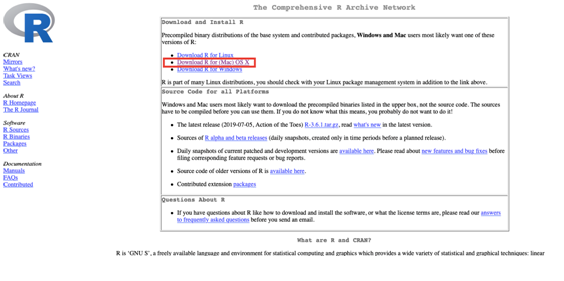
\includegraphics[width=1\linewidth]{figures/mac_R_1} \caption{\label{fig:mac1} Download R para Mac}\label{fig:mac1}
\end{figure}

\begin{enumerate}
\def\labelenumi{\arabic{enumi})}
\setcounter{enumi}{1}
\tightlist
\item
  Baixe o pacote R-3.6.1.pkg clicando no link indicado no retângulo vermelho na Figura \ref{fig:mac2}. Note que o 3.6.1 é o número da versão mais recente disponível no momento da confecção desse material.
\end{enumerate}

\begin{figure}
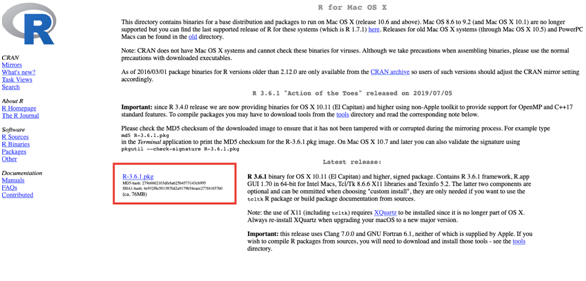
\includegraphics[width=1\linewidth]{figures/mac_R_2} \caption{\label{fig:mac2} Download R para Mac }\label{fig:mac2}
\end{figure}

\begin{enumerate}
\def\labelenumi{\arabic{enumi})}
\setcounter{enumi}{2}
\tightlist
\item
  Caso você não tenha configurado a pasta de descargas, o pacote será baixado na pasta ``Downloads'', como mostrado na seguinte Figura \ref{fig:mac3}. Observe que dois arquivos são baixados, clique duas vezes no arquivo ``R-3.6.1.pkg'' para abrir o assistente de instalação que o guiará durante o processo.
\end{enumerate}

\begin{figure}
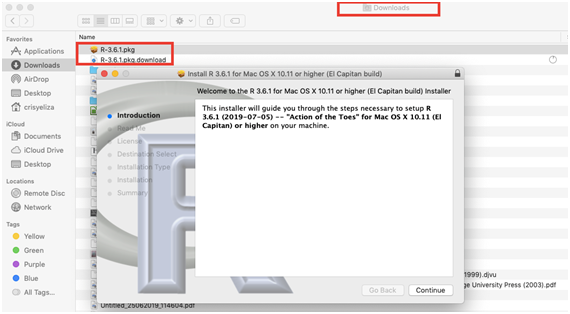
\includegraphics[width=1\linewidth]{figures/mac_R_3} \caption{\label{fig:mac3} Pasta para instalação}\label{fig:mac3}
\end{figure}

\begin{enumerate}
\def\labelenumi{\arabic{enumi})}
\setcounter{enumi}{3}
\tightlist
\item
  Acompanhe os passos indicados pelo instalador (Figura \ref{fig:mac4}).
\end{enumerate}

\begin{figure}
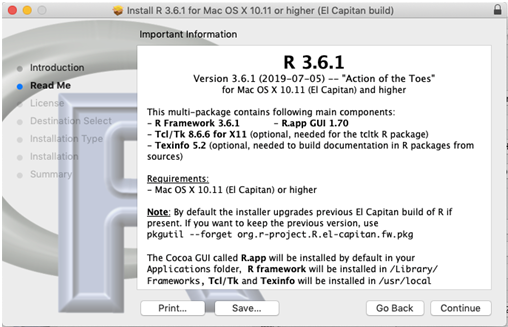
\includegraphics[width=1\linewidth]{figures/mac_R_4} \caption{\label{fig:mac4} Instalação}\label{fig:mac4}
\end{figure}

\begin{enumerate}
\def\labelenumi{\arabic{enumi})}
\setcounter{enumi}{4}
\tightlist
\item
  Deve concordar com os termos da licença, clique em ``Agree'' (Figura \ref{fig:mac5}).

  \begin{figure}
  
\includegraphics[width=1\linewidth]{figures/mac_R_5} \caption{\label{fig:mac5} Instalação}\label{fig:mac5}
  \end{figure}
\item
  Selecione o lugar onde instalará o programa, no caso de ter o disco particionado e assim desejar instalar em uma parte específica. Caso contrário, continue (Figura \ref{fig:mac6} e \ref{fig:mac7}).
\end{enumerate}

\begin{figure}

\includegraphics[width=1\linewidth]{figures/mac_R_6} \caption{\label{fig:mac6} Instalação}\label{fig:mac6}
\end{figure}

\begin{figure}

\includegraphics[width=1\linewidth]{figures/mac_R_7} \caption{\label{fig:mac7} Instalação}\label{fig:mac7}
\end{figure}

\begin{enumerate}
\def\labelenumi{\arabic{enumi})}
\setcounter{enumi}{6}
\tightlist
\item
  Para finalizar a instalação, o assistente lhe pedirá nome de usuário e senha do seu notebook, como apresentado na Figura \ref{fig:mac8}.
\end{enumerate}

\begin{figure}
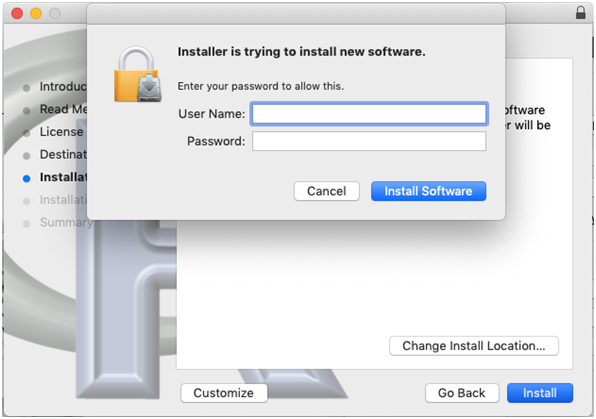
\includegraphics[width=1\linewidth]{figures/mac_R_8} \caption{\label{fig:mac8} Instalação}\label{fig:mac8}
\end{figure}

\begin{enumerate}
\def\labelenumi{\arabic{enumi})}
\setcounter{enumi}{7}
\tightlist
\item
  Pronto, agora o software R será instalado, como na Figura \ref{fig:mac9}, e quando terminar, aparecerá uma janela como apresentado na Figura \ref{fig:mac10}.
\end{enumerate}

\begin{figure}
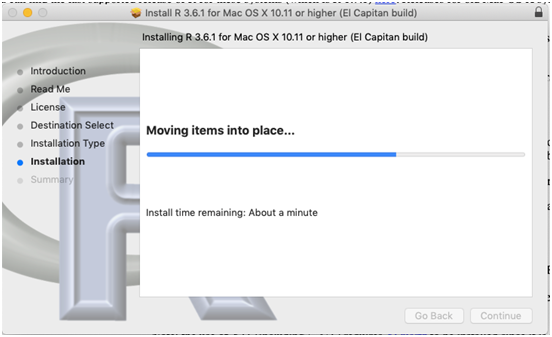
\includegraphics[width=1\linewidth]{figures/mac_R_9} \caption{\label{fig:mac9} Instalação}\label{fig:mac9}
\end{figure}

\begin{figure}

\includegraphics[width=1\linewidth]{figures/mac_R_10} \caption{\label{fig:mac10} Instalação}\label{fig:mac10}
\end{figure}

\hypertarget{para-linux}{%
\subsubsection{Para Linux}\label{para-linux}}

A instalação do R no Linux depende da distribuição utilizada. Entre neste \href{https://cran.r-project.org/}{link} para acessar a página do R e clique em Download R for Linux, como no link destacado em retângulo vermelho na Figura \ref{fig:linux1}. Em seguida, clique no link referente à distribuição utilizada (Figura \ref{fig:linux2}).

\begin{figure}

\includegraphics[width=1\linewidth]{figures/install_R_linux} \caption{\label{fig:linux1}Download em Linux}\label{fig:linux1}
\end{figure}

\begin{figure}
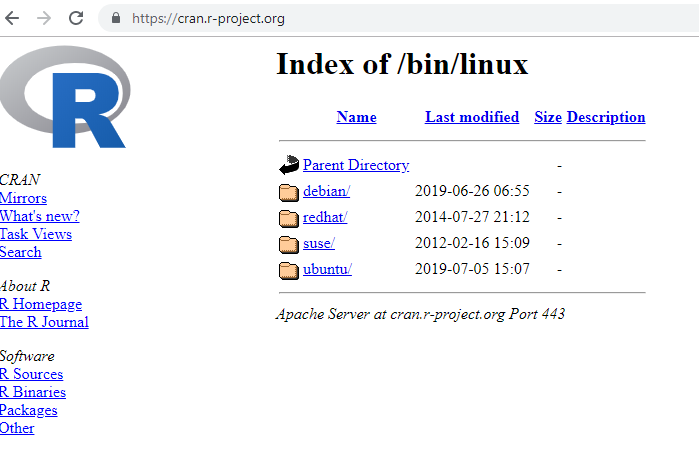
\includegraphics[width=1\linewidth]{figures/install_R_linux2} \caption{\label{fig:linux2}Download em Linux}\label{fig:linux2}
\end{figure}

\hypertarget{instalauxe7uxe3o-rstudio}{%
\subsection{Instalação RStudio}\label{instalauxe7uxe3o-rstudio}}

O RStudio é um conjunto de ferramentas integradas projetadas (IDE - Integrated Development Environment) da linguagem R para auxiliar na produtividade ao utilizar o R.

\hypertarget{para-windows-1}{%
\subsubsection{Para Windows}\label{para-windows-1}}

\begin{enumerate}
\def\labelenumi{\arabic{enumi})}
\tightlist
\item
  Entre neste \href{https://www.rstudio.com/products/rstudio/download/}{link} e clique em Download como em destaque na Figura \ref{fig:rswindows1}.
\end{enumerate}

\begin{figure}
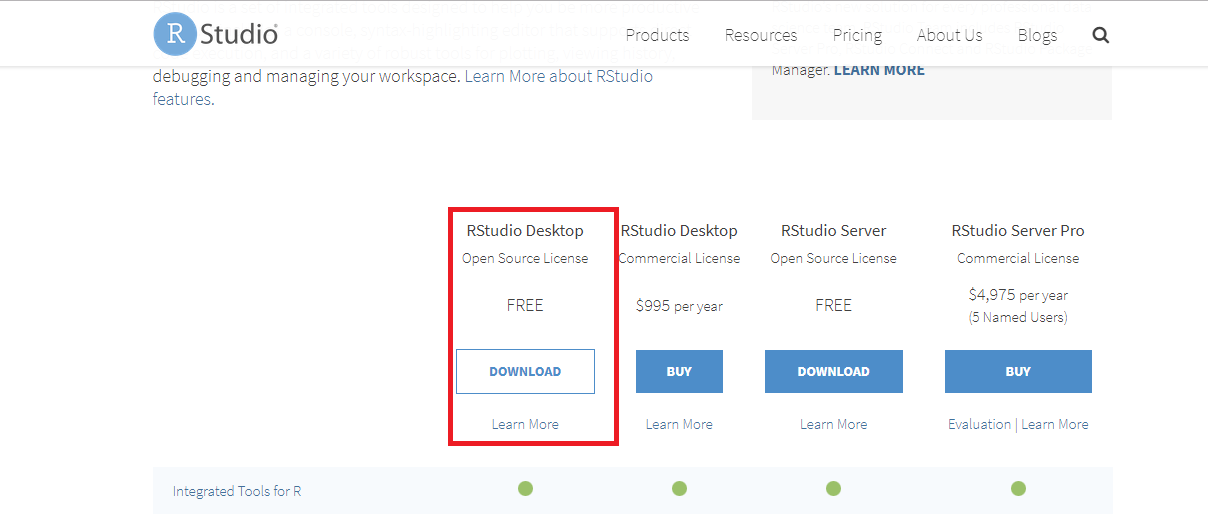
\includegraphics[width=1\linewidth]{figures/install_Rstudio1} \caption{\label{fig:rswindows1}Site para download do RStudio}\label{fig:rswindows1}
\end{figure}

\begin{enumerate}
\def\labelenumi{\arabic{enumi})}
\setcounter{enumi}{1}
\tightlist
\item
  Clique no instalador em destaque na Figura \ref{fig:rswindows2}.
\end{enumerate}

\begin{figure}
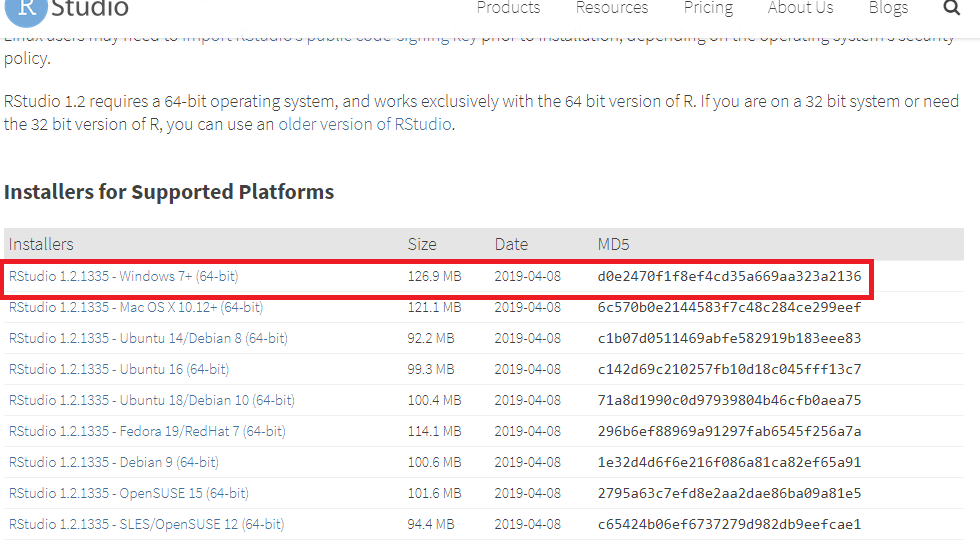
\includegraphics[width=1\linewidth]{figures/install_Rstudio2} \caption{\label{fig:rswindows2}Link para download do RStudio}\label{fig:rswindows2}
\end{figure}

\begin{enumerate}
\def\labelenumi{\arabic{enumi})}
\setcounter{enumi}{2}
\tightlist
\item
  Ao clicar no link, será feito o download do instalador e salvo na pasta de interesse. No caso da Figura \ref{fig:rswindows3}, o instalador está na pasta Downloads. Dê dois cliques no botão esquerdo no arquivo para iniciar o download do arquivo.
\end{enumerate}

\begin{figure}
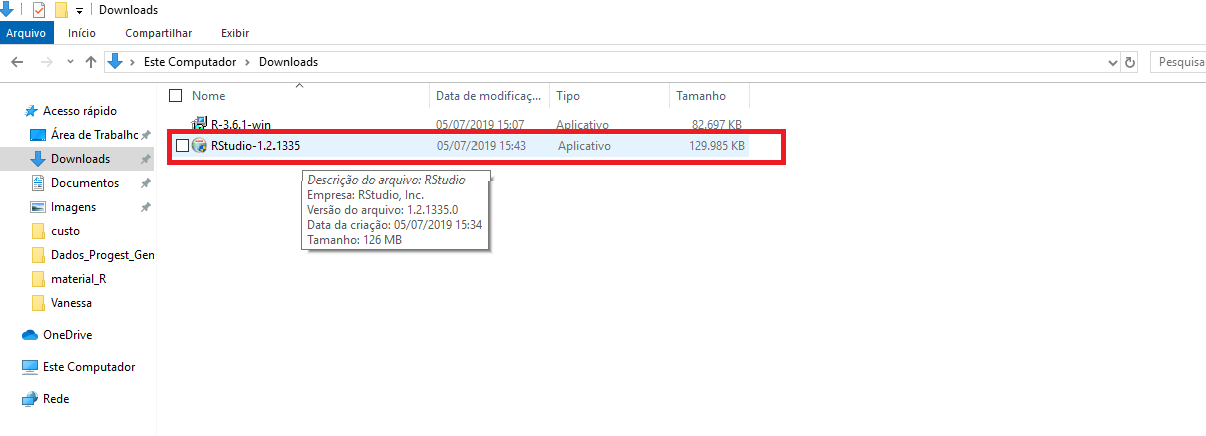
\includegraphics[width=1\linewidth]{figures/install_Rstudio3} \caption{\label{fig:rswindows3} Instalador}\label{fig:rswindows3}
\end{figure}

\begin{enumerate}
\def\labelenumi{\arabic{enumi})}
\setcounter{enumi}{3}
\tightlist
\item
  Clique em ``Próximo'' nas próximas janelas e na última ``Instalar'', como nas Figuras \ref{fig:rswindows4} a \ref{fig:rswindows6}.
\end{enumerate}

\begin{figure}
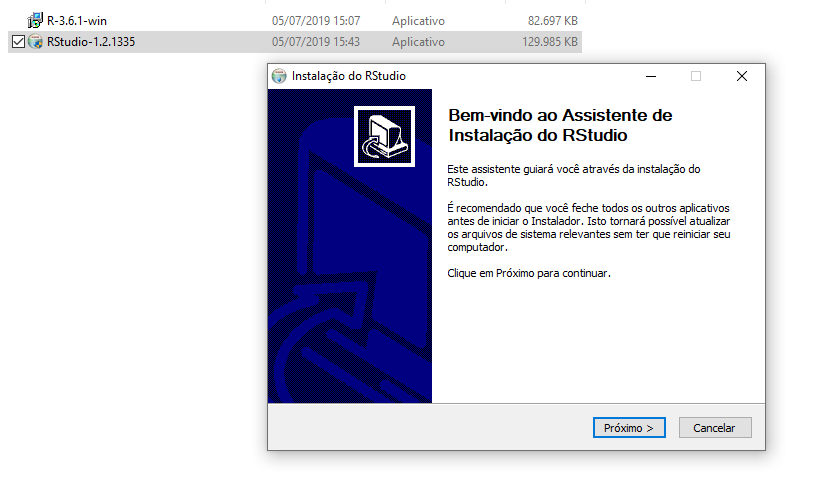
\includegraphics[width=1\linewidth]{figures/install_Rstudio4} \caption{\label{fig:rswindows4} Instalação}\label{fig:rswindows4}
\end{figure}

\begin{figure}
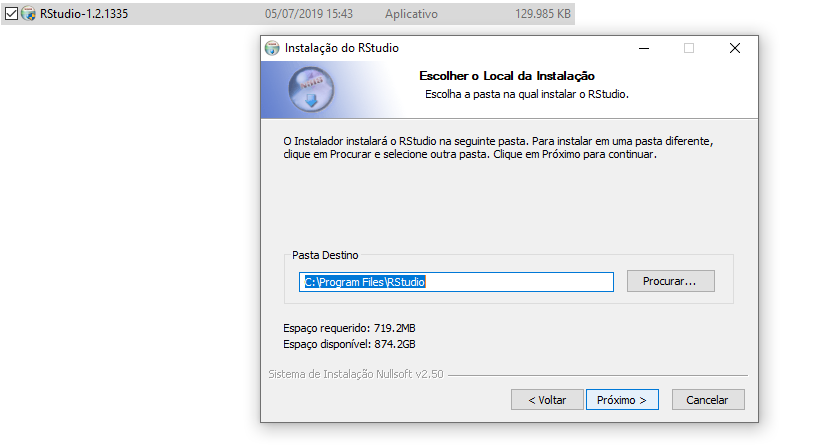
\includegraphics[width=1\linewidth]{figures/install_Rstudio5} \caption{\label{fig:rswindows5} Instalação}\label{fig:rswindows5}
\end{figure}

\begin{figure}
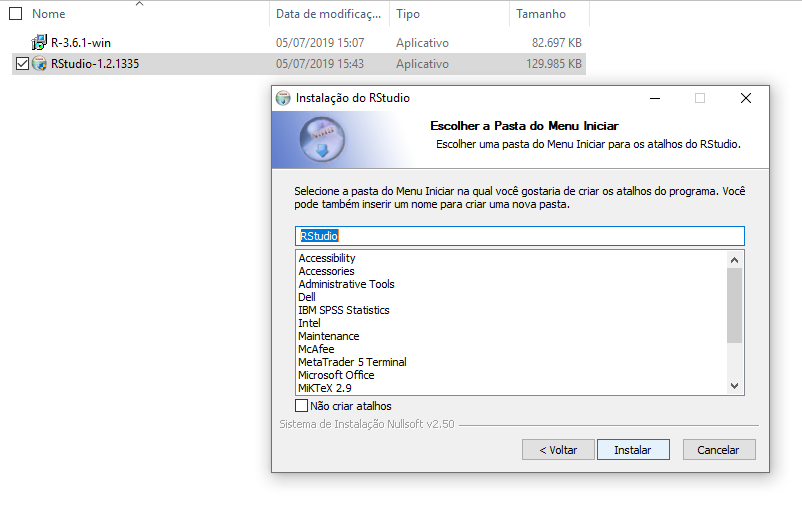
\includegraphics[width=1\linewidth]{figures/install_Rstudio6} \caption{\label{fig:rswindows6} Instalação}\label{fig:rswindows6}
\end{figure}

\begin{enumerate}
\def\labelenumi{\arabic{enumi})}
\setcounter{enumi}{4}
\tightlist
\item
  Pronto, a instalação será iniciada, como na Figura \ref{fig:rswindows7}.
\end{enumerate}

\begin{figure}
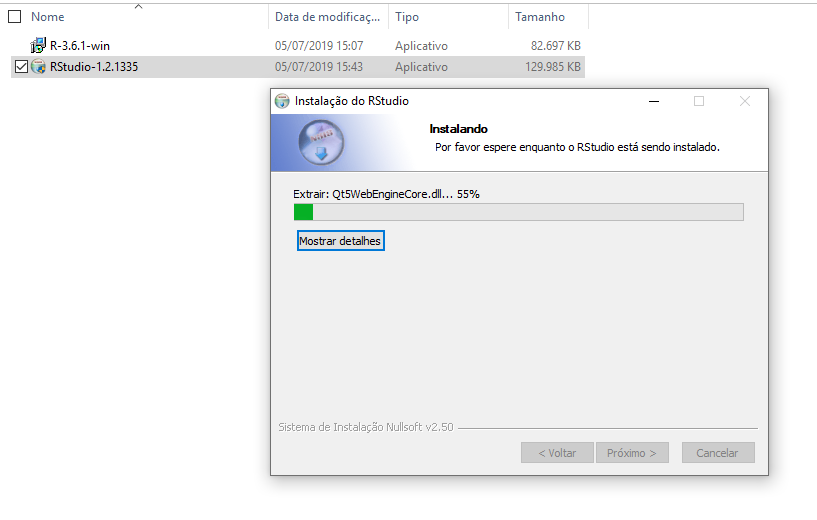
\includegraphics[width=1\linewidth]{figures/install_Rstudio7} \caption{\label{fig:rswindows7} Instalação}\label{fig:rswindows7}
\end{figure}

\hypertarget{para-mac-1}{%
\subsubsection{Para MAC}\label{para-mac-1}}

\begin{enumerate}
\def\labelenumi{\arabic{enumi})}
\tightlist
\item
  Entre neste \href{https://www.rstudio.com/products/rstudio/download/}{link} e clique em Download como em destaque na Figura \ref{fig:rsmac1}.
\end{enumerate}

\begin{figure}
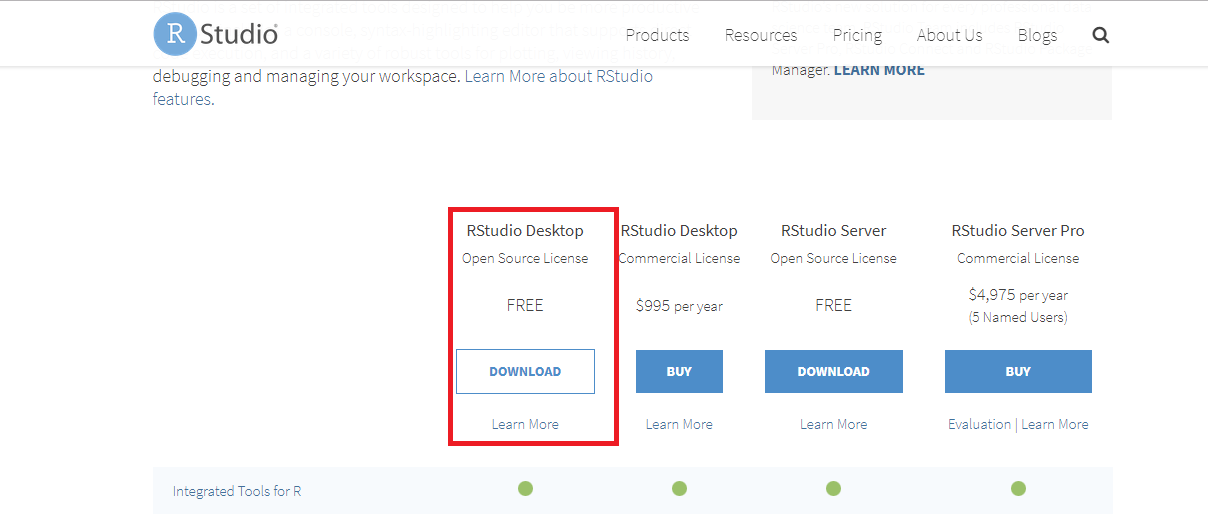
\includegraphics[width=1\linewidth]{figures/install_Rstudio1} \caption{\label{fig:rsmac1}Site para download do RStudio}\label{fig:rsmac1}
\end{figure}

\begin{enumerate}
\def\labelenumi{\arabic{enumi})}
\setcounter{enumi}{1}
\tightlist
\item
  Clique no instalador como destacado na Figura \ref{fig:rsmac2}.
\end{enumerate}

\begin{figure}
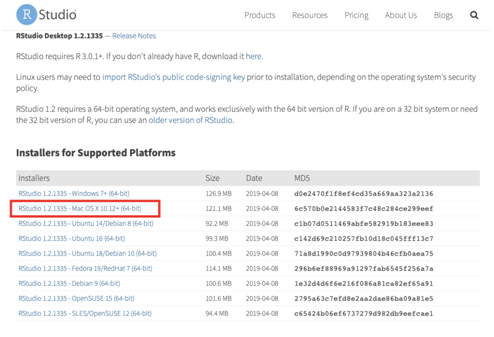
\includegraphics[width=1\linewidth]{figures/mac_RSt_1} \caption{\label{fig:rsmac2}Site para download do RStudio para Mac}\label{fig:rsmac2}
\end{figure}

\begin{enumerate}
\def\labelenumi{\arabic{enumi})}
\setcounter{enumi}{2}
\tightlist
\item
  Ao clicar no link, será feito o download do instalador e salvo na pasta de interesse. Caso você não tenha configurado a pasta de descargas, o instalador ficará na pasta ``Downloads'', como na Figura \ref{fig:rsmac3}.
\end{enumerate}

\begin{figure}
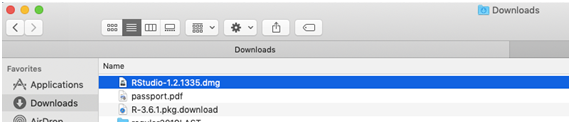
\includegraphics[width=1\linewidth]{figures/mac_RSt_2} \caption{\label{fig:rsmac3} Instalador salvo em pasta}\label{fig:rsmac3}
\end{figure}

\begin{enumerate}
\def\labelenumi{\arabic{enumi})}
\setcounter{enumi}{3}
\tightlist
\item
  Clicando duas vezes no arquivo ``RStudio-1.2.1335.dmg'' (versãos mais atual do RStudio), será feita a descarga do mesmo abrindo a janela conforme na Figura \ref{fig:rsmac4}. Clique no aplicativo de RStudio destacado em vermelho também na Figura \ref{fig:rsmac4}.
\end{enumerate}

\begin{figure}
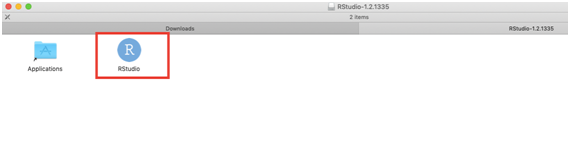
\includegraphics[width=1\linewidth]{figures/mac_RSt_3} \caption{\label{fig:rsmac4} Instalação}\label{fig:rsmac4}
\end{figure}

\begin{enumerate}
\def\labelenumi{\arabic{enumi})}
\setcounter{enumi}{4}
\tightlist
\item
  O instalador pode perguntar se está seguro que o aplicativo será baixado da internet e clique em ``Open'' (Figura \ref{fig:rsmac5}).
\end{enumerate}

\begin{figure}
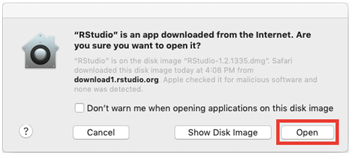
\includegraphics[width=1\linewidth]{figures/mac_RSt_4} \caption{\label{fig:rsmac5} Instalação}\label{fig:rsmac5}
\end{figure}

\begin{enumerate}
\def\labelenumi{\arabic{enumi})}
\setcounter{enumi}{5}
\tightlist
\item
  Pronto! Imediatamente abre o RStudio, como na Figura \ref{fig:rsmac6}, e você já pode utilizar.
\end{enumerate}

\begin{figure}
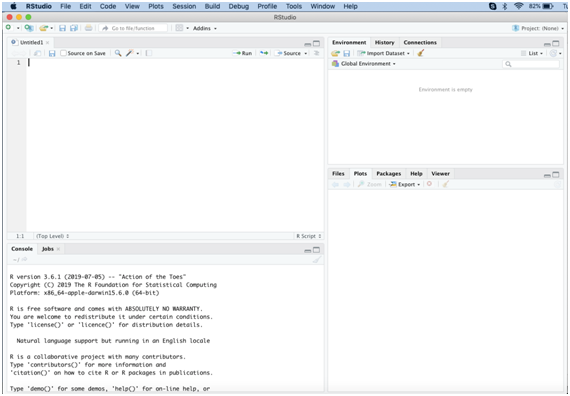
\includegraphics[width=1\linewidth]{figures/mac_RSt_5} \caption{\label{fig:rsmac6} Instalação}\label{fig:rsmac6}
\end{figure}

\hypertarget{para-linux-1}{%
\subsubsection{Para Linux}\label{para-linux-1}}

\begin{enumerate}
\def\labelenumi{\arabic{enumi})}
\tightlist
\item
  Entre neste \href{https://www.rstudio.com/products/rstudio/download/}{link} e clique em Download como em destaque na Figura \ref{fig:rslinux1}.
\end{enumerate}

\begin{figure}
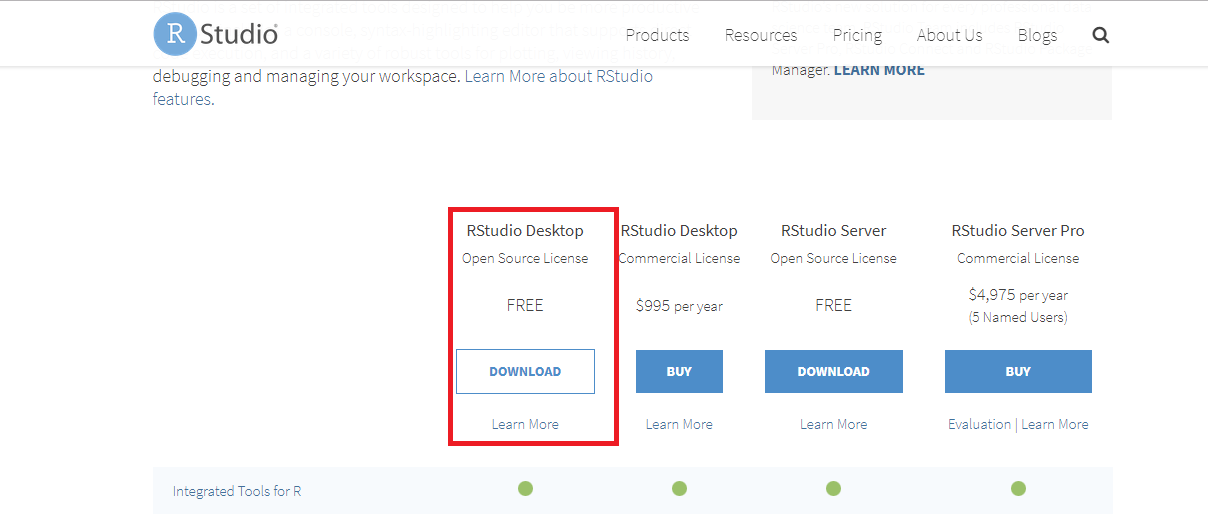
\includegraphics[width=1\linewidth]{figures/install_Rstudio1} \caption{\label{fig:rslinux1}Site para download do RStudio}\label{fig:rslinux1}
\end{figure}

\begin{enumerate}
\def\labelenumi{\arabic{enumi})}
\setcounter{enumi}{1}
\tightlist
\item
  Clique no link referente à distribuição utilizada (Figura \ref{fig:rslinux2}).

  \begin{figure}
  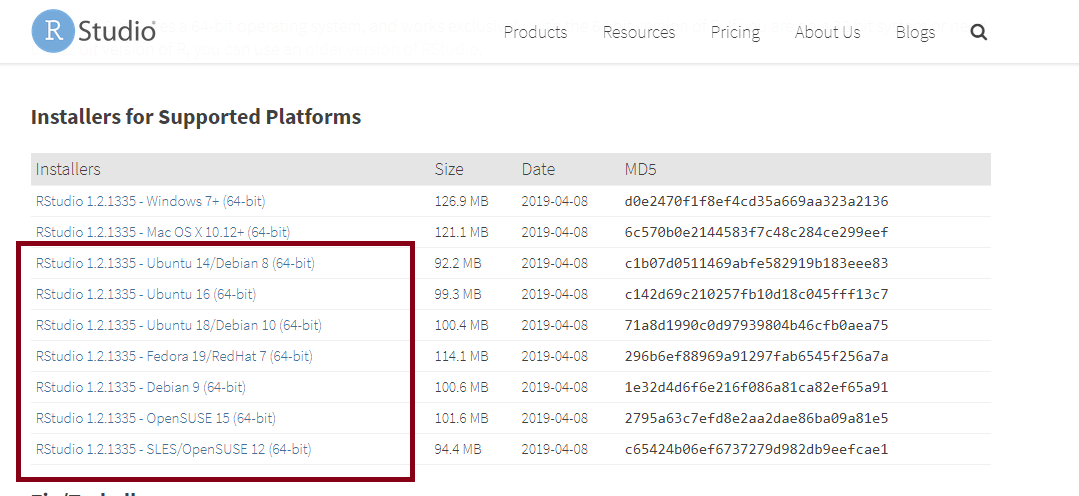
\includegraphics[width=1\linewidth]{figures/install_Rstudio_linux} \caption{\label{fig:rslinux2} Download do RStudio}\label{fig:rslinux2}
  \end{figure}
\end{enumerate}

\hypertarget{primeiros-passos-com-r-e-rstudio.}{%
\section{Primeiros passos com R e RStudio.}\label{primeiros-passos-com-r-e-rstudio.}}

\hypertarget{primeiros-contatos-com-rstudio}{%
\subsection{Primeiros contatos com RStudio}\label{primeiros-contatos-com-rstudio}}

O RStudio é um conjunto de ferramentas integradas projetadas (IDE - Integrated Development Environment) da linguagem R para editar e executar os códigos em R.

Tem quatro áreas, conforme a Figura \ref{fig:telarstudio1}.

\begin{figure}
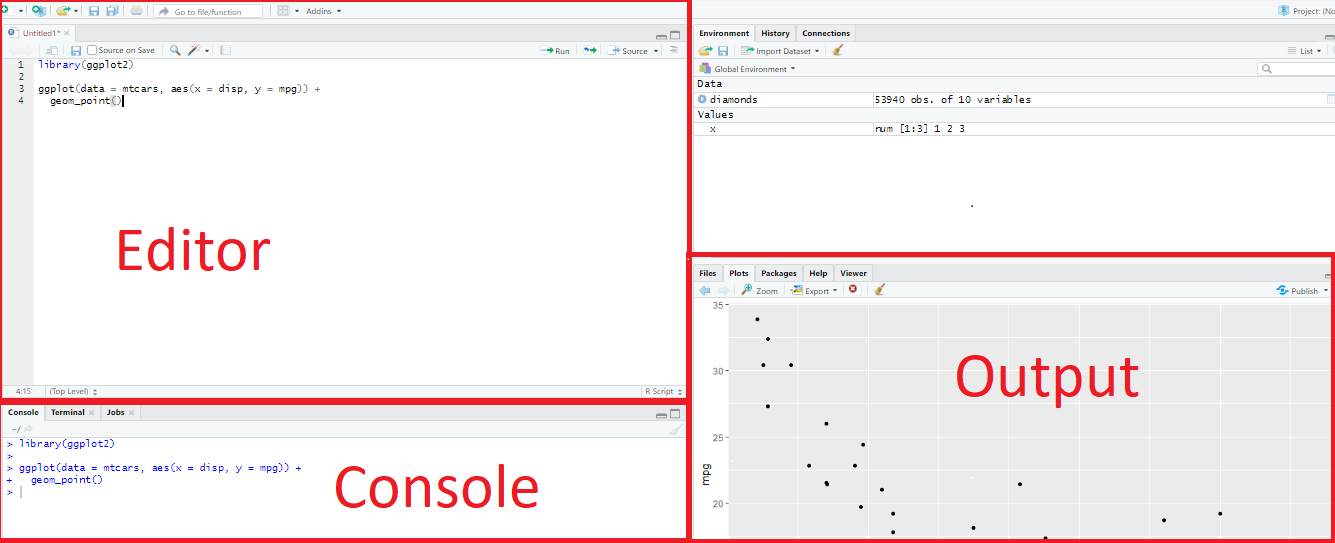
\includegraphics[width=1\linewidth]{figures/rstudio1} \caption{\label{fig:rstudio1} Visualização do RStudio}\label{fig:telarstudio1}
\end{figure}

A seguir descrevemos melhor os painéis e abas do RStudio:

\begin{itemize}
\item
  Editor/Scripts: É onde escrever os códigos. Arquivos do tipo .R.
\item
  Console: Executar os comandos e ver os resultados.
\item
  Enviroment: Painel com todos os objetos criados.
\item
  History: História dos comandos executados.
\item
  Files: Navegar em pastas e arquivos.
\item
  Plots: Onde os gráficos serão apresentados.
\item
  Packages: Pacotes instalados (sem ticar) e habilitados (ticados).
\item
  Help: Retorna o tutorial de ajuda do comando solicitado com help() ou ?comando. Ver melhor como pedir ajuda no R no final desse capítulo.
\end{itemize}

O usuário pode alterar a aparência do RStudio, como fonte e cor. Como exemplo, as Figuras \ref{fig:telarstudio2} e \ref{fig:telarstudio3} apresentam os passos para mudar o tema do script, no exemplo, deixar com fundo preto.

\begin{figure}
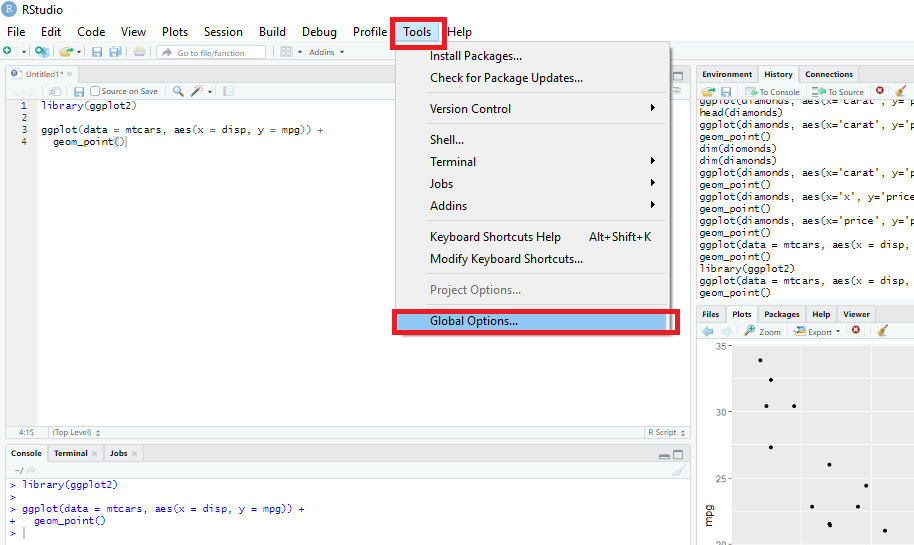
\includegraphics[width=1\linewidth]{figures/rstudio2} \caption{\label{fig:rstudio2} Ferramentas de aparência do RStudio}\label{fig:telarstudio2}
\end{figure}

\begin{figure}
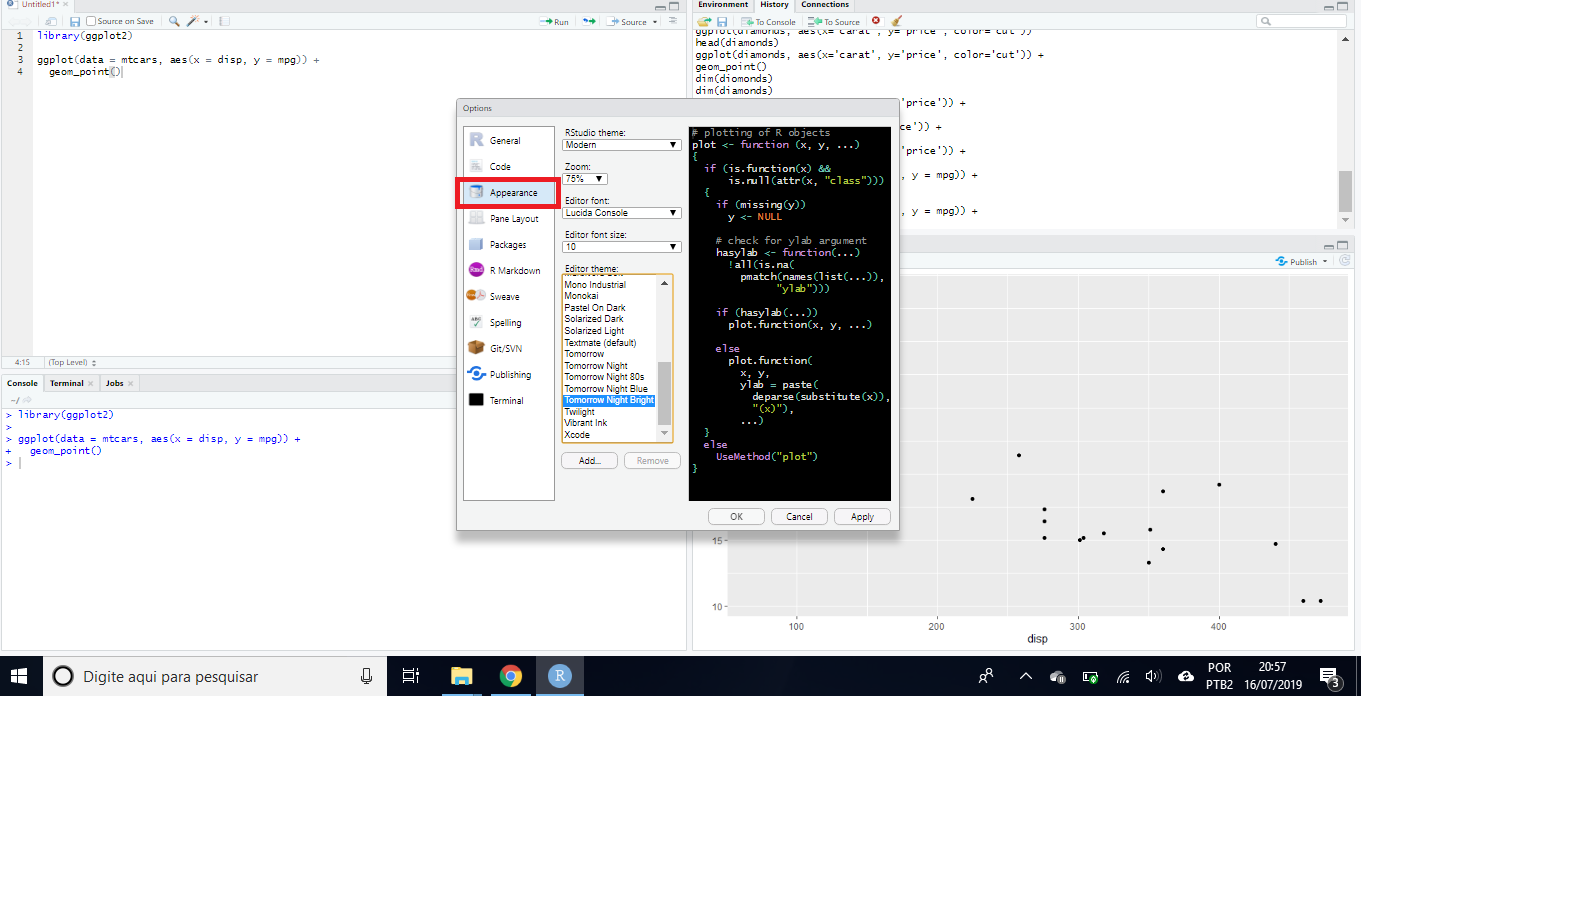
\includegraphics[width=1\linewidth]{figures/rstudio3} \caption{\label{fig:rstudio3} Ferramentas de aparência do RStudio}\label{fig:telarstudio3}
\end{figure}

Ainda no menu Tools --\textgreater{} Global Options --\textgreater{} Pane Layout, o usuário pode organizar a ordem dos quadrantes do RStudio, como apresentado nas Figuras \ref{fig:telarstudio4}, \ref{fig:telarstudio5} e \ref{fig:telarstudio6}. No exemplo, o painel console foi transferido para o lado do painel Script, o que facilita a visualização dos comandos rodados.

\begin{figure}
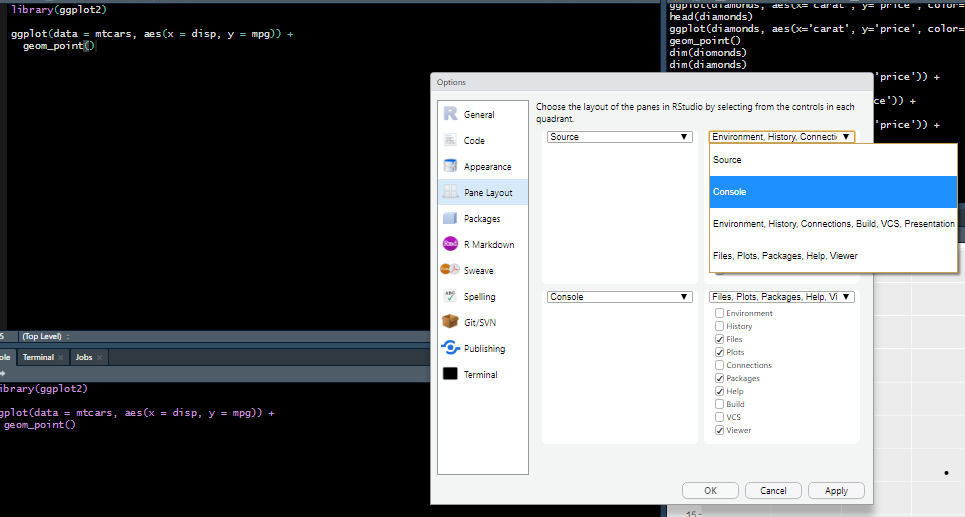
\includegraphics[width=1\linewidth]{figures/rstudio4} \caption{\label{fig:rstudio4} Ferramentas de aparência do RStudio}\label{fig:telarstudio4}
\end{figure}

\begin{figure}
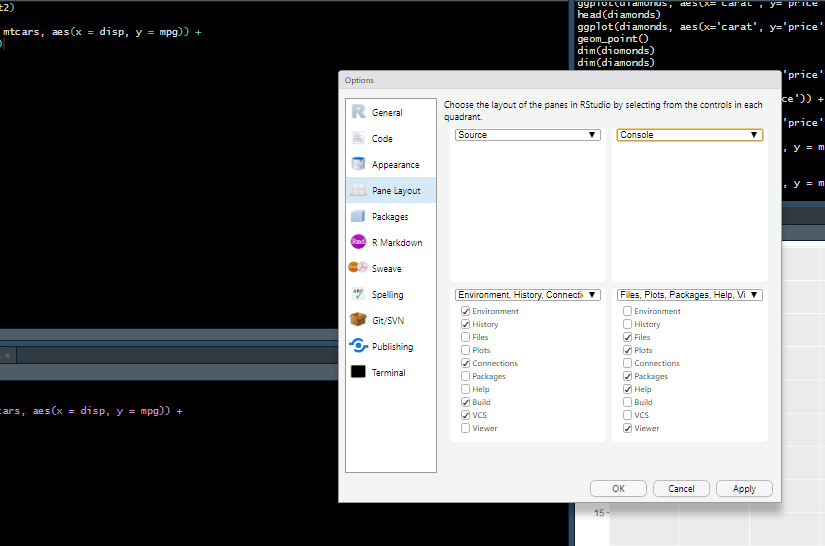
\includegraphics[width=1\linewidth]{figures/rstudio5} \caption{\label{fig:rstudio5} Ferramentas de aparência do RStudio}\label{fig:telarstudio5}
\end{figure}

\begin{figure}
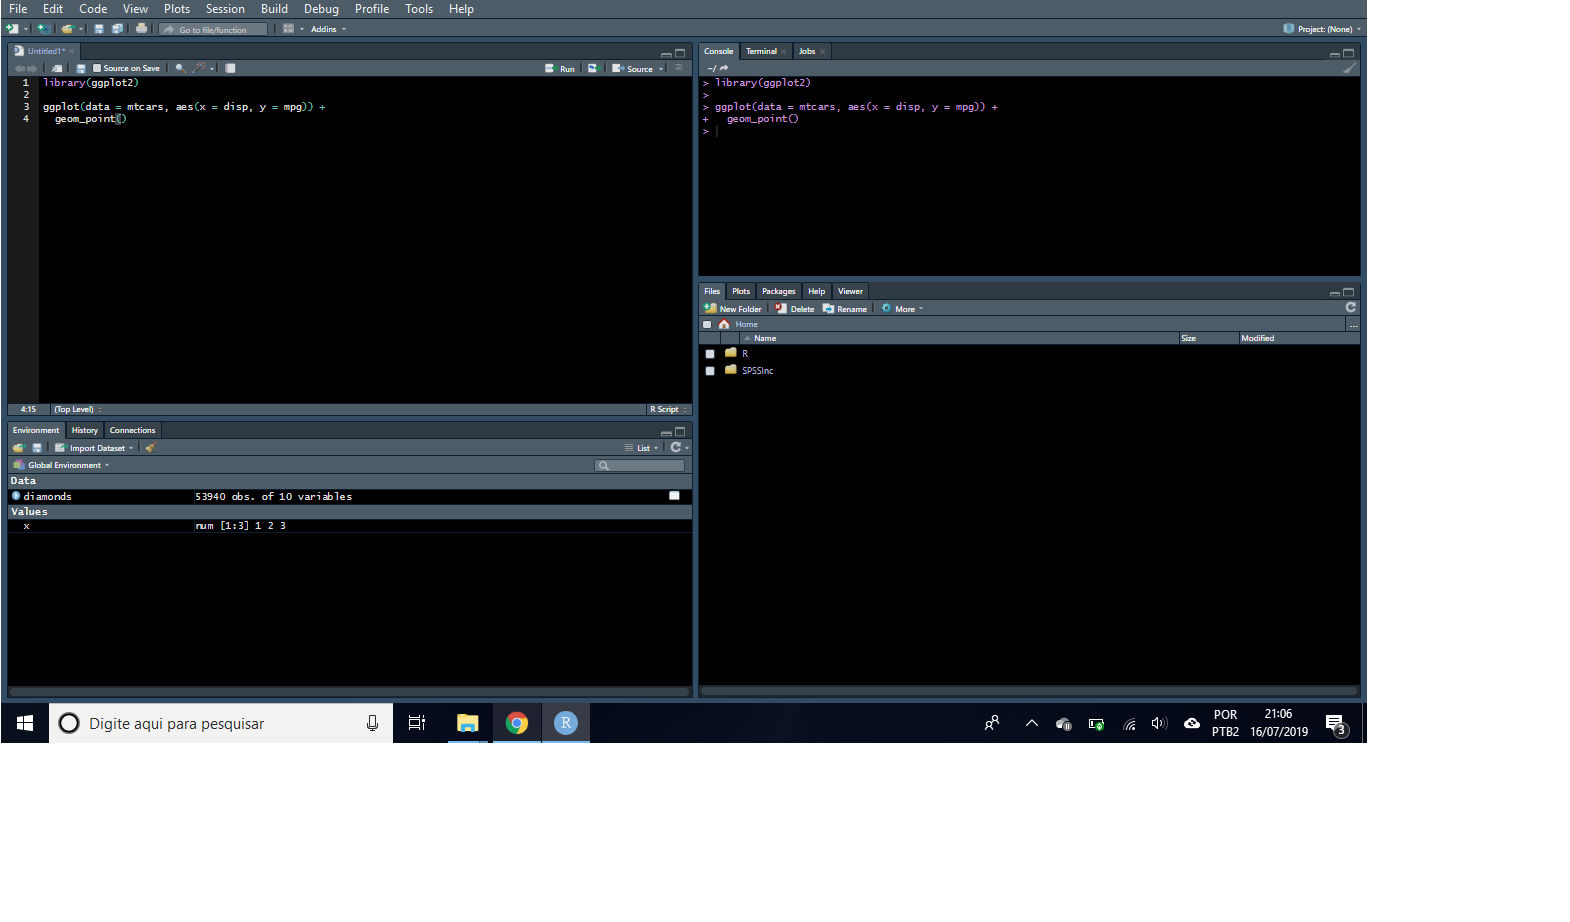
\includegraphics[width=1\linewidth]{figures/rstudio6} \caption{\label{fig:rstudio6} Ferramentas de aparência do RStudio}\label{fig:telarstudio6}
\end{figure}

\hypertarget{projetos}{%
\subsubsection{Projetos}\label{projetos}}

Uma funcionalidade importante é a criação de projetos, permitindo dividir o trabalho em múltiplos ambientes, cada um com o seu diretório, documentos e workspace.

Para criar um projeto, os seguintes passos podem ser seguidos:

\begin{enumerate}
\def\labelenumi{\arabic{enumi})}
\item
  Clique na opção ``File'' do menu, e então em ``New Project''.
\item
  Clique em ``New Directory''.
\item
  Clique em ``New Project''.
\item
  Escreva o nome do diretório (pasta) onde deseja manter seu projeto, ex ``my\_project''.
\item
  Clique no botão ``Create Project''.
\end{enumerate}

Para criar um novo script para escrever os códigos, vá em File -\textgreater{} New File -\textgreater{} R Script

\hypertarget{boas-pruxe1ticas}{%
\subsubsection{Boas práticas}\label{boas-pruxe1ticas}}

Comente bem o seu código: É possível fazer comentários usando o símbolo `\#'. É sempre bom explicar o que uma variável armazena, o que uma função faz, porque alguns parâmetros são passados para uma determinada função, qual é o objetivo de um trecho de código, etc.

Evite linhas de código muito longas: Usar linhas de código mais curtas ajuda na leitura do código.

Escreva um código organizado. Por exemplo, adote um padrão no uso de minúsculas e maiúsculas, uma lógica única na organização de pastas e arquivos, pode ser adotada uma breve descrição (como comentário) indicando o que um determinado script faz.

Carregue todos os pacotes que irá usar sempre no início do arquivo: Quando alguém abrir o seu código será fácil identificar quais são os pacotes que devem ser instalados e quais dependências podem existir.

\hypertarget{primeiros-passos-no-r}{%
\subsection{Primeiros passos no R}\label{primeiros-passos-no-r}}

Posso escrever o código no Script e submeter ao apertar o botão ``Run'' ou com o atalho no teclado Cmd/Ctrl+Enter.

\hypertarget{r-como-calculadora}{%
\subsubsection{R como calculadora}\label{r-como-calculadora}}

\begin{enumerate}
\def\labelenumi{\arabic{enumi})}
\tightlist
\item
  Operadores
\end{enumerate}

\begin{Shaded}
\begin{Highlighting}[]
\CommentTok{#adição}
\DecValTok{10}\OperatorTok{+}\DecValTok{15}
\end{Highlighting}
\end{Shaded}

\begin{verbatim}
## [1] 25
\end{verbatim}

\begin{Shaded}
\begin{Highlighting}[]
\CommentTok{#subtração}
\DecValTok{10-2}
\end{Highlighting}
\end{Shaded}

\begin{verbatim}
## [1] 8
\end{verbatim}

\begin{Shaded}
\begin{Highlighting}[]
\CommentTok{#multiplicação}
\DecValTok{2}\OperatorTok{*}\DecValTok{10}
\end{Highlighting}
\end{Shaded}

\begin{verbatim}
## [1] 20
\end{verbatim}

\begin{Shaded}
\begin{Highlighting}[]
\CommentTok{#divisão}
\DecValTok{30}\OperatorTok{/}\DecValTok{2}
\end{Highlighting}
\end{Shaded}

\begin{verbatim}
## [1] 15
\end{verbatim}

\begin{Shaded}
\begin{Highlighting}[]
\CommentTok{#raiz quadrada}
\KeywordTok{sqrt}\NormalTok{(}\DecValTok{4}\NormalTok{)}
\end{Highlighting}
\end{Shaded}

\begin{verbatim}
## [1] 2
\end{verbatim}

\begin{Shaded}
\begin{Highlighting}[]
\CommentTok{#potência}
\DecValTok{2}\OperatorTok{^}\DecValTok{2}
\end{Highlighting}
\end{Shaded}

\begin{verbatim}
## [1] 4
\end{verbatim}

Se você digitar um comando incompleto, como 10 *, o R mostrará um +. Isso não tem a ver com a soma e apenas que o R está esperando você completar seu comando. Termine seu comando ou aperte Esc para recomeçar.
Vale também ressaltar que se você digitar um comando que o R não reconhece, ele retornará uma mensagem de erro e você pode digitar outro comando normalmente em seguida.

\hypertarget{atribuiuxe7uxe3o}{%
\subsubsection{Atribuição}\label{atribuiuxe7uxe3o}}

Podemos salvar valores dentro de um objeto, que é simplemente um nome que guarda um valor, vetor, matriz, lista ou base de dados.

Para atribuir a um objeto, o sinal de atribuição é \texttt{=} ou \texttt{\textless{}-} (preferível).

Exemplos:

\begin{Shaded}
\begin{Highlighting}[]
\NormalTok{x <-}\StringTok{ }\DecValTok{10}\OperatorTok{/}\DecValTok{2}
\NormalTok{x}
\end{Highlighting}
\end{Shaded}

\begin{verbatim}
## [1] 5
\end{verbatim}

\begin{Shaded}
\begin{Highlighting}[]
\NormalTok{X}
\end{Highlighting}
\end{Shaded}

\begin{verbatim}
## Error in eval(expr, envir, enclos): objeto 'X' não encontrado
\end{verbatim}

Por que tivemos um erro acima?

O R é case sensitive, isto é, faz a diferenciação entre as letras minúsculas e maiúsculas. Portanto, x é diferente de X.

\hypertarget{objetos-em-r}{%
\subsubsection{Objetos em R}\label{objetos-em-r}}

Existem cinco classes básicas no R:

\begin{itemize}
\item
  character: ``UAH!''
\item
  numeric: 0.95 (números reais)
\item
  integer: 100515 (inteiros)
\item
  complex: 2 + 5i (números complexos, a + bi)
\item
  logical: TRUE (booleanos, TRUE/FALSE)
\end{itemize}

Vamos atribuir a x a string banana.

\begin{Shaded}
\begin{Highlighting}[]
\NormalTok{x <-}\StringTok{ }\NormalTok{banana }
\end{Highlighting}
\end{Shaded}

\begin{verbatim}
## Error in eval(expr, envir, enclos): objeto 'banana' não encontrado
\end{verbatim}

\begin{Shaded}
\begin{Highlighting}[]
\NormalTok{x <-}\StringTok{ "banana"}
\NormalTok{x}
\end{Highlighting}
\end{Shaded}

\begin{verbatim}
## [1] "banana"
\end{verbatim}

O primeiro caso (x \textless- banana) não deu certo, pois ele entendeu que estamos atribuindo a x outro objeto banana, que não foi declarado. Para atribuir o string banana à x, precisamos colocar entre aspas ou aspas simples. Uma string sem aspas é entendido como um objeto, veja abaixo:

\begin{Shaded}
\begin{Highlighting}[]
\NormalTok{banana <-}\StringTok{ }\DecValTok{30}
\NormalTok{x <-}\StringTok{ }\NormalTok{banana}
\NormalTok{x}
\end{Highlighting}
\end{Shaded}

\begin{verbatim}
## [1] 30
\end{verbatim}

Para saber a classe de um objetivo, use a função class().

\begin{Shaded}
\begin{Highlighting}[]
\NormalTok{y <-}\StringTok{ "ola"}
\KeywordTok{class}\NormalTok{(y)}
\end{Highlighting}
\end{Shaded}

\begin{verbatim}
## [1] "character"
\end{verbatim}

\begin{Shaded}
\begin{Highlighting}[]
\NormalTok{x <-}\StringTok{ }\FloatTok{2.5}
\KeywordTok{class}\NormalTok{(x)}
\end{Highlighting}
\end{Shaded}

\begin{verbatim}
## [1] "numeric"
\end{verbatim}

\hypertarget{apagar-objetos}{%
\subsubsection{Apagar objetos}\label{apagar-objetos}}

E se eu quiser apagar um objeto?

\begin{Shaded}
\begin{Highlighting}[]
\NormalTok{x <-}\StringTok{ }\DecValTok{20}
\NormalTok{x}
\end{Highlighting}
\end{Shaded}

\begin{verbatim}
## [1] 20
\end{verbatim}

\begin{Shaded}
\begin{Highlighting}[]
\KeywordTok{remove}\NormalTok{(x)}
\NormalTok{x}
\end{Highlighting}
\end{Shaded}

\begin{verbatim}
## Error in eval(expr, envir, enclos): objeto 'x' não encontrado
\end{verbatim}

E se eu quiser limpar o console - apaga todos os objetos atribuidos até aqui:

\begin{Shaded}
\begin{Highlighting}[]
\KeywordTok{rm}\NormalTok{(}\DataTypeTok{list=}\KeywordTok{ls}\NormalTok{())}
\end{Highlighting}
\end{Shaded}

\hypertarget{vetor}{%
\subsubsection{Vetor}\label{vetor}}

Como atribuir varios valores a um objeto? Para entrar com vários números (ou nomes, ou qualquer outro grupo de coisas), precisamos usar uma função para dizer ao programa que os valores serão combinados em um único vetor.

\begin{Shaded}
\begin{Highlighting}[]
\NormalTok{x <-}\StringTok{ }\KeywordTok{c}\NormalTok{(}\DecValTok{2}\NormalTok{,}\DecValTok{3}\NormalTok{,}\DecValTok{4}\NormalTok{)}
\NormalTok{x}
\end{Highlighting}
\end{Shaded}

\begin{verbatim}
## [1] 2 3 4
\end{verbatim}

\begin{Shaded}
\begin{Highlighting}[]
\NormalTok{y <-}\StringTok{ }\KeywordTok{seq}\NormalTok{(}\DecValTok{1}\NormalTok{,}\DecValTok{10}\NormalTok{)}
\NormalTok{y}
\end{Highlighting}
\end{Shaded}

\begin{verbatim}
##  [1]  1  2  3  4  5  6  7  8  9 10
\end{verbatim}

\begin{Shaded}
\begin{Highlighting}[]
\NormalTok{z <-}\StringTok{ }\KeywordTok{rep}\NormalTok{(}\DecValTok{1}\NormalTok{,}\DecValTok{10}\NormalTok{)}
\NormalTok{z}
\end{Highlighting}
\end{Shaded}

\begin{verbatim}
##  [1] 1 1 1 1 1 1 1 1 1 1
\end{verbatim}

\begin{Shaded}
\begin{Highlighting}[]
\NormalTok{a <-}\StringTok{ }\DecValTok{1}\OperatorTok{:}\DecValTok{10}
\NormalTok{a}
\end{Highlighting}
\end{Shaded}

\begin{verbatim}
##  [1]  1  2  3  4  5  6  7  8  9 10
\end{verbatim}

\begin{Shaded}
\begin{Highlighting}[]
\NormalTok{bicho <-}\KeywordTok{c}\NormalTok{(}\StringTok{"macaco"}\NormalTok{,}\StringTok{"pato"}\NormalTok{,}\StringTok{"galinha"}\NormalTok{,}\StringTok{"porco"}\NormalTok{)}
\NormalTok{bicho}
\end{Highlighting}
\end{Shaded}

\begin{verbatim}
## [1] "macaco"  "pato"    "galinha" "porco"
\end{verbatim}

E se quisermos visualizar o conteúdo da posição 2 no vetor bicho?

\begin{Shaded}
\begin{Highlighting}[]
\NormalTok{bicho[}\DecValTok{2}\NormalTok{]}
\end{Highlighting}
\end{Shaded}

\begin{verbatim}
## [1] "pato"
\end{verbatim}

As operações vetoriais podem ser realizadas de maneira bastante intuitiva. Como exemplos:

\begin{Shaded}
\begin{Highlighting}[]
\NormalTok{x <-}\StringTok{ }\KeywordTok{c}\NormalTok{(}\DecValTok{2}\NormalTok{,}\DecValTok{3}\NormalTok{,}\DecValTok{4}\NormalTok{)}
\NormalTok{x}
\end{Highlighting}
\end{Shaded}

\begin{verbatim}
## [1] 2 3 4
\end{verbatim}

\begin{Shaded}
\begin{Highlighting}[]
\NormalTok{ops <-}\StringTok{ }\NormalTok{x}\DecValTok{-1}
\NormalTok{ops}
\end{Highlighting}
\end{Shaded}

\begin{verbatim}
## [1] 1 2 3
\end{verbatim}

\begin{Shaded}
\begin{Highlighting}[]
\NormalTok{k <-}\StringTok{ }\NormalTok{x}\OperatorTok{*}\DecValTok{2}
\NormalTok{k}
\end{Highlighting}
\end{Shaded}

\begin{verbatim}
## [1] 4 6 8
\end{verbatim}

Vamos agora considerar um vetor de pesos em kg e altura em metros de 6 pessoas.

\begin{Shaded}
\begin{Highlighting}[]
\NormalTok{peso <-}\StringTok{ }\KeywordTok{c}\NormalTok{(}\DecValTok{62}\NormalTok{, }\DecValTok{70}\NormalTok{, }\DecValTok{52}\NormalTok{, }\DecValTok{98}\NormalTok{, }\DecValTok{90}\NormalTok{, }\DecValTok{70}\NormalTok{)}
\NormalTok{peso}
\end{Highlighting}
\end{Shaded}

\begin{verbatim}
## [1] 62 70 52 98 90 70
\end{verbatim}

\begin{Shaded}
\begin{Highlighting}[]
\NormalTok{altura <-}\StringTok{ }\KeywordTok{c}\NormalTok{(}\FloatTok{1.70}\NormalTok{, }\FloatTok{1.82}\NormalTok{, }\FloatTok{1.75}\NormalTok{, }\FloatTok{1.94}\NormalTok{, }\FloatTok{1.84}\NormalTok{, }\FloatTok{1.61}\NormalTok{)}
\NormalTok{altura}
\end{Highlighting}
\end{Shaded}

\begin{verbatim}
## [1] 1.70 1.82 1.75 1.94 1.84 1.61
\end{verbatim}

Vale mencionar que o separador de decimais no R é . (ponto)!

Como calcularia o IMC? Lembrando que o IMC é dado pelo peso (em kg) dividido pela altura (em metros) ao quadrado.

\begin{Shaded}
\begin{Highlighting}[]
\NormalTok{imc <-}\StringTok{ }\NormalTok{peso}\OperatorTok{/}\NormalTok{(altura}\OperatorTok{^}\DecValTok{2}\NormalTok{)}
\NormalTok{imc}
\end{Highlighting}
\end{Shaded}

\begin{verbatim}
## [1] 21.45329 21.13271 16.97959 26.03890 26.58318 27.00513
\end{verbatim}

Para saber o tamanho do vetor, use a função length().

\begin{Shaded}
\begin{Highlighting}[]
\KeywordTok{length}\NormalTok{(imc)}
\end{Highlighting}
\end{Shaded}

\begin{verbatim}
## [1] 6
\end{verbatim}

\hypertarget{matrizes}{%
\subsubsection{Matrizes}\label{matrizes}}

Matrizes são vetores numéricos com duas dimensões, que são simplesmente a linha e a coluna às quais o elemento pertence.

\begin{Shaded}
\begin{Highlighting}[]
\NormalTok{x <-}\StringTok{ }\KeywordTok{matrix}\NormalTok{(}\KeywordTok{seq}\NormalTok{(}\DecValTok{1}\NormalTok{,}\DecValTok{16}\NormalTok{), }\DataTypeTok{nrow=}\DecValTok{4}\NormalTok{,}\DataTypeTok{ncol=}\DecValTok{4}\NormalTok{)}
\NormalTok{x}
\end{Highlighting}
\end{Shaded}

\begin{verbatim}
##      [,1] [,2] [,3] [,4]
## [1,]    1    5    9   13
## [2,]    2    6   10   14
## [3,]    3    7   11   15
## [4,]    4    8   12   16
\end{verbatim}

Note que os números de 1 a 16 foram dispostos na matriz coluna por coluna ou seja, preenchendo de cima para baixo e depois da esquerda para a direita.

Como sei qual elemento está na segunda linha e terceira coluna da matriz x?

\begin{Shaded}
\begin{Highlighting}[]
\NormalTok{x[}\DecValTok{2}\NormalTok{,}\DecValTok{3}\NormalTok{]}
\end{Highlighting}
\end{Shaded}

\begin{verbatim}
## [1] 10
\end{verbatim}

\begin{Shaded}
\begin{Highlighting}[]
\NormalTok{x[}\DecValTok{3}\NormalTok{,  ]   }\CommentTok{# seleciona a 3ª linha}
\end{Highlighting}
\end{Shaded}

\begin{verbatim}
## [1]  3  7 11 15
\end{verbatim}

\begin{Shaded}
\begin{Highlighting}[]
\NormalTok{x[ , }\DecValTok{2}\NormalTok{]   }\CommentTok{# seleciona a 2ª coluna}
\end{Highlighting}
\end{Shaded}

\begin{verbatim}
## [1] 5 6 7 8
\end{verbatim}

\begin{Shaded}
\begin{Highlighting}[]
\NormalTok{x[}\DecValTok{1}\NormalTok{, }\DecValTok{2}\NormalTok{]   }\CommentTok{# seleciona o elemento da primeira linha e segunda coluna}
\end{Highlighting}
\end{Shaded}

\begin{verbatim}
## [1] 5
\end{verbatim}

E se eu quiser substituir a primeira linha por (13,15,19,30)?

\begin{Shaded}
\begin{Highlighting}[]
\NormalTok{x[}\DecValTok{1}\NormalTok{,] <-}\StringTok{ }\KeywordTok{c}\NormalTok{(}\DecValTok{13}\NormalTok{,}\DecValTok{15}\NormalTok{,}\DecValTok{19}\NormalTok{,}\DecValTok{30}\NormalTok{)}

\NormalTok{x}
\end{Highlighting}
\end{Shaded}

\begin{verbatim}
##      [,1] [,2] [,3] [,4]
## [1,]   13   15   19   30
## [2,]    2    6   10   14
## [3,]    3    7   11   15
## [4,]    4    8   12   16
\end{verbatim}

Seja o vetor d

\begin{Shaded}
\begin{Highlighting}[]
\NormalTok{d <-}\StringTok{ }\KeywordTok{c}\NormalTok{(}\DecValTok{128}\NormalTok{,}\DecValTok{124}\NormalTok{,}\DecValTok{213}\NormalTok{,}\DecValTok{234}\NormalTok{)}
\end{Highlighting}
\end{Shaded}

E se quisermos substituir a terceira coluna por d?

\begin{Shaded}
\begin{Highlighting}[]
\NormalTok{x[,}\DecValTok{3}\NormalTok{] <-}\StringTok{ }\NormalTok{d}
\end{Highlighting}
\end{Shaded}

Qual a dimensao da matriz x?

Vimos que para vetor usamos o comando length(). Serve para matriz? Vamos testar:

\begin{Shaded}
\begin{Highlighting}[]
\KeywordTok{length}\NormalTok{(x)}
\end{Highlighting}
\end{Shaded}

\begin{verbatim}
## [1] 16
\end{verbatim}

Note que retorna o número de colunas vezes o número de linhas (4*4=16). Mas o que quero saber é o numero de linhas e de colunas. Para isso, o comando é \texttt{dim()}.

\begin{Shaded}
\begin{Highlighting}[]
\KeywordTok{dim}\NormalTok{(x)}
\end{Highlighting}
\end{Shaded}

\begin{verbatim}
## [1] 4 4
\end{verbatim}

Para concatenar linhas em uma matriz, podemos usar o comando \texttt{rbind()}:

\begin{Shaded}
\begin{Highlighting}[]
\NormalTok{vet <-}\StringTok{ }\KeywordTok{c}\NormalTok{(}\DecValTok{2}\NormalTok{,}\DecValTok{20}\NormalTok{,}\DecValTok{12}\NormalTok{,}\DecValTok{34}\NormalTok{)}
\NormalTok{x2 <-}\StringTok{ }\KeywordTok{rbind}\NormalTok{(x,vet)}
\NormalTok{x2}
\end{Highlighting}
\end{Shaded}

\begin{verbatim}
##     [,1] [,2] [,3] [,4]
##       13   15  128   30
##        2    6  124   14
##        3    7  213   15
##        4    8  234   16
## vet    2   20   12   34
\end{verbatim}

Para concatenar colunas em uma matriz, podemos usar o comando \texttt{cbind()}:

\begin{Shaded}
\begin{Highlighting}[]
\NormalTok{v2 <-}\StringTok{ }\KeywordTok{c}\NormalTok{(}\DecValTok{25}\NormalTok{,}\DecValTok{10}\NormalTok{,}\DecValTok{15}\NormalTok{,}\DecValTok{4}\NormalTok{) }
\NormalTok{x3 <-}\StringTok{ }\KeywordTok{cbind}\NormalTok{(x,v2)}
\NormalTok{x3}
\end{Highlighting}
\end{Shaded}

\begin{verbatim}
##                   v2
## [1,] 13 15 128 30 25
## [2,]  2  6 124 14 10
## [3,]  3  7 213 15 15
## [4,]  4  8 234 16  4
\end{verbatim}

\hypertarget{fator}{%
\subsubsection{Fator}\label{fator}}

Fatores podem ser vistos como vetores de inteiros que possuem rótulos (labels). Eles são úteis para representar uma variável categórica (nominal e ordinal).

\begin{Shaded}
\begin{Highlighting}[]
\NormalTok{sexo <-}\StringTok{ }\KeywordTok{c}\NormalTok{(}\StringTok{"M"}\NormalTok{, }\StringTok{"H"}\NormalTok{, }\StringTok{"H"}\NormalTok{, }\StringTok{"H"}\NormalTok{, }\StringTok{"M"}\NormalTok{, }\StringTok{"M"}\NormalTok{, }\StringTok{"H"}\NormalTok{)}
\NormalTok{sex <-}\StringTok{ }\KeywordTok{as.factor}\NormalTok{(sexo)}
\NormalTok{sex}
\end{Highlighting}
\end{Shaded}

\begin{verbatim}
## [1] M H H H M M H
## Levels: H M
\end{verbatim}

\begin{Shaded}
\begin{Highlighting}[]
\KeywordTok{levels}\NormalTok{(sex)}
\end{Highlighting}
\end{Shaded}

\begin{verbatim}
## [1] "H" "M"
\end{verbatim}

\hypertarget{data-frame}{%
\subsubsection{Data frame}\label{data-frame}}

Trata-se de uma ``tabela de dados'' onde as colunas são as variáveis e as linhas são os registros. Essas colunas podem ser de classes diferentes.
Essa é a grande diferença entre data.frame's e matrizes (matriz é só numerica).

Posso criar um data frame no R com os vetores, por exemplo:

\begin{Shaded}
\begin{Highlighting}[]
\NormalTok{ID <-}\StringTok{ }\KeywordTok{seq}\NormalTok{(}\DecValTok{1}\NormalTok{,}\DecValTok{6}\NormalTok{)}
\NormalTok{pes <-}\StringTok{ }\KeywordTok{c}\NormalTok{(}\DecValTok{62}\NormalTok{, }\DecValTok{70}\NormalTok{, }\DecValTok{52}\NormalTok{, }\DecValTok{98}\NormalTok{, }\DecValTok{90}\NormalTok{, }\DecValTok{70}\NormalTok{)}
\NormalTok{alt <-}\StringTok{ }\KeywordTok{c}\NormalTok{(}\FloatTok{1.70}\NormalTok{, }\FloatTok{1.82}\NormalTok{, }\FloatTok{1.75}\NormalTok{, }\FloatTok{1.94}\NormalTok{, }\FloatTok{1.84}\NormalTok{, }\FloatTok{1.61}\NormalTok{)}
\NormalTok{imc <-}\StringTok{ }\NormalTok{pes}\OperatorTok{/}\NormalTok{(alt}\OperatorTok{^}\DecValTok{2}\NormalTok{)}
\NormalTok{dados <-}\StringTok{ }\KeywordTok{data.frame}\NormalTok{(}\DataTypeTok{ID=}\NormalTok{ID,}\DataTypeTok{peso=}\NormalTok{pes,}\DataTypeTok{altura=}\NormalTok{alt, }\DataTypeTok{imc=}\NormalTok{imc)}
\NormalTok{dados}
\end{Highlighting}
\end{Shaded}

\begin{verbatim}
##   ID peso altura      imc
## 1  1   62   1.70 21.45329
## 2  2   70   1.82 21.13271
## 3  3   52   1.75 16.97959
## 4  4   98   1.94 26.03890
## 5  5   90   1.84 26.58318
## 6  6   70   1.61 27.00513
\end{verbatim}

Posso pensar que o data frame tem a mesma ideia de matriz. Quero olhar os dados de altura. Sei que altura está na coluna 3.

\begin{Shaded}
\begin{Highlighting}[]
\NormalTok{dados[,}\DecValTok{3}\NormalTok{]}
\end{Highlighting}
\end{Shaded}

\begin{verbatim}
## [1] 1.70 1.82 1.75 1.94 1.84 1.61
\end{verbatim}

Mas existe uma maneira mais fácil de selecionar a variável de interesse sem ter que saber em qual coluna ela está.
Por ser um data frame, posso usar \texttt{\$} da seguinte maneira:

\begin{Shaded}
\begin{Highlighting}[]
\NormalTok{dados}\OperatorTok{$}\NormalTok{altura}
\end{Highlighting}
\end{Shaded}

\begin{verbatim}
## [1] 1.70 1.82 1.75 1.94 1.84 1.61
\end{verbatim}

Putz, esqueci de colocar a variável de grupo no data frame. Tenho que criar tudo de novo? Não:

\begin{Shaded}
\begin{Highlighting}[]
\NormalTok{gr <-}\StringTok{ }\KeywordTok{c}\NormalTok{(}\KeywordTok{rep}\NormalTok{(}\DecValTok{1}\NormalTok{,}\DecValTok{3}\NormalTok{),}\KeywordTok{rep}\NormalTok{(}\DecValTok{2}\NormalTok{,}\DecValTok{3}\NormalTok{))}
\NormalTok{dados}\OperatorTok{$}\NormalTok{grupo <-}\StringTok{ }\NormalTok{gr}

\NormalTok{dados}
\end{Highlighting}
\end{Shaded}

\begin{verbatim}
##   ID peso altura      imc grupo
## 1  1   62   1.70 21.45329     1
## 2  2   70   1.82 21.13271     1
## 3  3   52   1.75 16.97959     1
## 4  4   98   1.94 26.03890     2
## 5  5   90   1.84 26.58318     2
## 6  6   70   1.61 27.00513     2
\end{verbatim}

Veja que no ``dados\$grupo'' foi inserido o objeto ``gr''. Se ``gr'' não tivesse o mesmo número de linhas do data frame retornaria um erro.

\textbf{Funções úteis para data.frame:}

Ainda não falamos com muito detalhes sobre funções no R, faremos isso mais adiante. Mas por enquanto, considere que sejam nomes já salvos no R e que, ao colocar o objeto da base de dados (no nosso exemplo é \texttt{dados}) dentro dos parênteses, retorna algumas informações úteis sobre a base de dados. São algumas delas:

\begin{itemize}
\item
  head() - Mostra as primeiras 6 linhas.
\item
  tail() - Mostra as últimas 6 linhas.
\item
  dim() - Número de linhas e de colunas.
\item
  names() - Os nomes das colunas (variáveis).
\item
  str() - Estrutura do data.frame. Mostra, entre outras coisas, as classes de cada coluna.
\end{itemize}

\begin{Shaded}
\begin{Highlighting}[]
\KeywordTok{head}\NormalTok{(dados)}
\end{Highlighting}
\end{Shaded}

\begin{verbatim}
##   ID peso altura      imc grupo
## 1  1   62   1.70 21.45329     1
## 2  2   70   1.82 21.13271     1
## 3  3   52   1.75 16.97959     1
## 4  4   98   1.94 26.03890     2
## 5  5   90   1.84 26.58318     2
## 6  6   70   1.61 27.00513     2
\end{verbatim}

\begin{Shaded}
\begin{Highlighting}[]
\KeywordTok{dim}\NormalTok{(dados)}
\end{Highlighting}
\end{Shaded}

\begin{verbatim}
## [1] 6 5
\end{verbatim}

\begin{Shaded}
\begin{Highlighting}[]
\KeywordTok{names}\NormalTok{(dados)}
\end{Highlighting}
\end{Shaded}

\begin{verbatim}
## [1] "ID"     "peso"   "altura" "imc"    "grupo"
\end{verbatim}

\begin{Shaded}
\begin{Highlighting}[]
\KeywordTok{str}\NormalTok{(dados)}
\end{Highlighting}
\end{Shaded}

\begin{verbatim}
## 'data.frame':	6 obs. of  5 variables:
##  $ ID    : int  1 2 3 4 5 6
##  $ peso  : num  62 70 52 98 90 70
##  $ altura: num  1.7 1.82 1.75 1.94 1.84 1.61
##  $ imc   : num  21.5 21.1 17 26 26.6 ...
##  $ grupo : num  1 1 1 2 2 2
\end{verbatim}

\hypertarget{operadores-luxf3gicos}{%
\subsubsection{Operadores lógicos}\label{operadores-luxf3gicos}}

A operação lógica nada mais é do que um teste que retorna verdadeiro (\texttt{TRUE}) ou falso (\texttt{FALSE}). Esses valores dois valores recebem uma classe especial: \texttt{logical}.

\begin{itemize}
\tightlist
\item
  Igual a: ==
\end{itemize}

Vamos ao testar se um valor é igual ao outro.

Exemplo:

\begin{Shaded}
\begin{Highlighting}[]
\DecValTok{10}\OperatorTok{==}\DecValTok{11}
\end{Highlighting}
\end{Shaded}

\begin{verbatim}
## [1] FALSE
\end{verbatim}

\begin{Shaded}
\begin{Highlighting}[]
\DecValTok{11}\OperatorTok{==}\DecValTok{11}
\end{Highlighting}
\end{Shaded}

\begin{verbatim}
## [1] TRUE
\end{verbatim}

No primeiro retornou \texttt{FALSE}, pois realmente 10 não é igual a 11 e no segundo caso acima retornou \texttt{TRUE}, pois realmente 11 é igual a 11.
De maneira análoga funciona para os operadores abaixo:

\begin{itemize}
\tightlist
\item
  Diferente de: !=
\end{itemize}

Exemplo:

\begin{Shaded}
\begin{Highlighting}[]
\DecValTok{10}\OperatorTok{!=}\DecValTok{11}
\end{Highlighting}
\end{Shaded}

\begin{verbatim}
## [1] TRUE
\end{verbatim}

\begin{itemize}
\item
  Maior que: \textgreater{}
\item
  Maior ou igual: \textgreater=
\item
  Menor que: \textless{}
\item
  Menor ou igual: \textless=
\end{itemize}

Exemplos:

\begin{Shaded}
\begin{Highlighting}[]
\DecValTok{10}\OperatorTok{>}\DecValTok{5}
\end{Highlighting}
\end{Shaded}

\begin{verbatim}
## [1] TRUE
\end{verbatim}

\begin{Shaded}
\begin{Highlighting}[]
\DecValTok{10}\OperatorTok{>=}\DecValTok{10}
\end{Highlighting}
\end{Shaded}

\begin{verbatim}
## [1] TRUE
\end{verbatim}

\begin{Shaded}
\begin{Highlighting}[]
\DecValTok{4}\OperatorTok{<}\DecValTok{4}
\end{Highlighting}
\end{Shaded}

\begin{verbatim}
## [1] FALSE
\end{verbatim}

\begin{Shaded}
\begin{Highlighting}[]
\DecValTok{4}\OperatorTok{<=}\DecValTok{4}
\end{Highlighting}
\end{Shaded}

\begin{verbatim}
## [1] TRUE
\end{verbatim}

\begin{itemize}
\tightlist
\item
  Um outro operador muito útil é o \texttt{\%in\%}. Com ele, podemos verificar se um valor está dentro de um vetor.
\end{itemize}

\begin{Shaded}
\begin{Highlighting}[]
\NormalTok{ex <-}\StringTok{ }\DecValTok{1}\OperatorTok{:}\DecValTok{15}
\DecValTok{3} \OperatorTok\StringTok{ }\NormalTok{ex}
\end{Highlighting}
\end{Shaded}

\begin{verbatim}
## [1] TRUE
\end{verbatim}

\begin{itemize}
\tightlist
\item
  E: \& - será verdadeiro se os dois forem TRUE
\end{itemize}

\begin{Shaded}
\begin{Highlighting}[]
\NormalTok{x <-}\StringTok{ }\DecValTok{15}
\NormalTok{x }\OperatorTok{>}\StringTok{ }\DecValTok{10} \OperatorTok{&}\StringTok{ }\NormalTok{x }\OperatorTok{<}\StringTok{ }\DecValTok{30}
\end{Highlighting}
\end{Shaded}

\begin{verbatim}
## [1] TRUE
\end{verbatim}

\begin{Shaded}
\begin{Highlighting}[]
\NormalTok{x }\OperatorTok{<}\StringTok{ }\DecValTok{10} \OperatorTok{&}\StringTok{ }\NormalTok{x }\OperatorTok{<}\StringTok{ }\DecValTok{30}
\end{Highlighting}
\end{Shaded}

\begin{verbatim}
## [1] FALSE
\end{verbatim}

\begin{itemize}
\tightlist
\item
  OU: \textbar{} - será verdadeiro se um dos dois forem TRUE
\end{itemize}

\begin{Shaded}
\begin{Highlighting}[]
\NormalTok{x <-}\StringTok{ }\DecValTok{15}
\NormalTok{x }\OperatorTok{>}\StringTok{ }\DecValTok{10} \OperatorTok{|}\StringTok{ }\NormalTok{x }\OperatorTok{<}\StringTok{ }\DecValTok{30}
\end{Highlighting}
\end{Shaded}

\begin{verbatim}
## [1] TRUE
\end{verbatim}

\begin{Shaded}
\begin{Highlighting}[]
\NormalTok{x }\OperatorTok{<}\StringTok{ }\DecValTok{10} \OperatorTok{|}\StringTok{ }\NormalTok{x }\OperatorTok{<}\StringTok{ }\DecValTok{30}
\end{Highlighting}
\end{Shaded}

\begin{verbatim}
## [1] TRUE
\end{verbatim}

\begin{itemize}
\tightlist
\item
  Negação: !
\end{itemize}

\begin{Shaded}
\begin{Highlighting}[]
\NormalTok{x <-}\StringTok{ }\DecValTok{15}
\OperatorTok{!}\NormalTok{x}\OperatorTok{<}\DecValTok{30}
\end{Highlighting}
\end{Shaded}

\begin{verbatim}
## [1] FALSE
\end{verbatim}

\hypertarget{dados-faltantes-infinitos-e-indefiniuxe7uxf5es-matemuxe1ticas}{%
\subsubsection{Dados faltantes, infinitos e indefinições matemáticas}\label{dados-faltantes-infinitos-e-indefiniuxe7uxf5es-matemuxe1ticas}}

\begin{itemize}
\tightlist
\item
  NA (Not Available): dado faltante/indisponível. Exemplo:
\end{itemize}

\begin{Shaded}
\begin{Highlighting}[]
\NormalTok{x <-}\StringTok{ }\KeywordTok{c}\NormalTok{(}\DecValTok{1}\NormalTok{,}\DecValTok{6}\NormalTok{,}\DecValTok{9}\NormalTok{)}
\NormalTok{x[}\DecValTok{4}\NormalTok{]}
\end{Highlighting}
\end{Shaded}

\begin{verbatim}
## [1] NA
\end{verbatim}

retornou \texttt{NA} porque não há elemento na posição 4 do vetor x.

\begin{itemize}
\tightlist
\item
  NaN (Not a Number): indefinições matemáticas. Como 0/0 e log(-1).
  Exemplo:
\end{itemize}

\begin{Shaded}
\begin{Highlighting}[]
\KeywordTok{log}\NormalTok{(}\OperatorTok{-}\DecValTok{10}\NormalTok{)}
\end{Highlighting}
\end{Shaded}

\begin{verbatim}
## [1] NaN
\end{verbatim}

\begin{itemize}
\tightlist
\item
  Inf (Infinito): número muito grande ou o limite matemático. Aceita sinal negativo -Inf.
  Exemplo:
\end{itemize}

\begin{Shaded}
\begin{Highlighting}[]
\DecValTok{10}\OperatorTok{^}\DecValTok{14321}
\end{Highlighting}
\end{Shaded}

\begin{verbatim}
## [1] Inf
\end{verbatim}

\hypertarget{condicionamento-if-e-else}{%
\subsubsection{Condicionamento : If e else}\label{condicionamento-if-e-else}}

As estruturas if e else servem para executar um código apenas se uma condição (teste lógico) for satisfeita.

\begin{Shaded}
\begin{Highlighting}[]
\NormalTok{a <-}\StringTok{ }\DecValTok{224}
\NormalTok{b <-}\StringTok{ }\DecValTok{225}
\ControlFlowTok{if}\NormalTok{ (a}\OperatorTok{==}\NormalTok{b) \{ }
\NormalTok{  v <-}\StringTok{ }\DecValTok{10}
\NormalTok{\} }\ControlFlowTok{else}\NormalTok{ \{}
\NormalTok{  v <-}\StringTok{ }\DecValTok{15}
\NormalTok{  \}}
\NormalTok{v}
\end{Highlighting}
\end{Shaded}

\begin{verbatim}
## [1] 15
\end{verbatim}

Veja que o R só executa o conteúdo das chaves \{\} se a expressão dentro dos parênteses () retornar \texttt{TRUE}.

Note que a condição de igualdade é representada por dois iguais ==. Como dito anteriormente, apenas um igual = é símbolo de atribuição (preferível \textless-).

Veja outro exemplo:

\begin{Shaded}
\begin{Highlighting}[]
\NormalTok{a <-}\StringTok{ }\DecValTok{224}
\NormalTok{b <-}\StringTok{ }\DecValTok{225}
\ControlFlowTok{if}\NormalTok{ (a}\OperatorTok{==}\NormalTok{b) \{ }
\NormalTok{  v <-}\StringTok{ }\DecValTok{10}
\NormalTok{\} }\ControlFlowTok{else} \ControlFlowTok{if}\NormalTok{ (a }\OperatorTok{>}\StringTok{ }\NormalTok{b) \{}
\NormalTok{  v <-}\StringTok{ }\DecValTok{15}
\NormalTok{  \} }\ControlFlowTok{else}\NormalTok{ \{}
\NormalTok{    v <-}\StringTok{ }\DecValTok{25}
\NormalTok{    \}}
\NormalTok{v}
\end{Highlighting}
\end{Shaded}

\begin{verbatim}
## [1] 25
\end{verbatim}

Veja que nesse exemplo gostaria de usar mais de duas condições e por isso usamos a estrutura intermediária else if.

\hypertarget{iterador-for}{%
\subsubsection{Iterador for}\label{iterador-for}}

O for serve para repetir uma mesma tarefa para um conjunto de valores diferentes. Cada repetição é chamada de iteração.

Como exemplo, considere o vetor atribuído ao objeto m como segue:

\begin{Shaded}
\begin{Highlighting}[]
\NormalTok{m <-}\StringTok{ }\KeywordTok{c}\NormalTok{(}\DecValTok{1}\NormalTok{,}\DecValTok{20}\NormalTok{,}\DecValTok{50}\NormalTok{,}\DecValTok{60}\NormalTok{,}\DecValTok{100}\NormalTok{)}
\end{Highlighting}
\end{Shaded}

Quero criar um novo vetor, p digamos, que seja formado por cada elemento
de m dividido por sua posição.

\begin{Shaded}
\begin{Highlighting}[]
\NormalTok{p <-}\StringTok{ }\OtherTok{NULL}
\ControlFlowTok{for}\NormalTok{ (i }\ControlFlowTok{in} \DecValTok{1}\OperatorTok{:}\StringTok{ }\KeywordTok{length}\NormalTok{(m))\{}
\NormalTok{  p[i] <-}\StringTok{ }\NormalTok{m[i]}\OperatorTok{/}\NormalTok{i}
\NormalTok{\}}
\NormalTok{p}
\end{Highlighting}
\end{Shaded}

\begin{verbatim}
## [1]  1.00000 10.00000 16.66667 15.00000 20.00000
\end{verbatim}

Note que primeiro definimos o objeto p, recebendo \texttt{NULL}. O \texttt{NULL} representa a ausência de um objeto e serve para já declarar algum objeto que receberá valor na sequência. No caso, ao rodar o for, o p é um vetor de tamanho 5 (tamanho do vetor m).

No exemplo, temos 5 iterações e para cada valor de i, correndo de 1 até 5 (tamanho de m), pegamos o valor de m na posição i e dividimos por sua posição. Assim formamos o vetor p.~

\hypertarget{funuxe7uxf5es}{%
\subsubsection{Funções}\label{funuxe7uxf5es}}

Funções no R são nomes que guardam um código de R. A ideia é que sempre que rodar a função com os seus argumentos, o código que ela guarda será executado e o resultado será retornado.

Já usamos anteriormente algumas funções que estão na base do R. Por exemplo, quando usamos \texttt{class()} para entender a classe do objeto que o R está entendendo. Colocamos um argumento dentro do parênteses e o R retornou qual a classe do objeto em questão. Relembre o que falamos ao perguntar ao R qual a classe do vetor oi criado:

\begin{Shaded}
\begin{Highlighting}[]
\NormalTok{oi <-}\StringTok{ }\KeywordTok{c}\NormalTok{(}\DecValTok{10}\NormalTok{,}\DecValTok{20}\NormalTok{,}\DecValTok{2}\NormalTok{,}\DecValTok{1}\NormalTok{,}\FloatTok{0.5}\NormalTok{)}
\KeywordTok{class}\NormalTok{(oi)}
\end{Highlighting}
\end{Shaded}

\begin{verbatim}
## [1] "numeric"
\end{verbatim}

Agora vamos conversar sobre outra função já criada e disponibilizada na base do R: \texttt{mean}. Essa função retorna a média do vetor que está em seu argumento. Vamos calcular a média dos valores do vetor oi:

\begin{Shaded}
\begin{Highlighting}[]
\KeywordTok{mean}\NormalTok{(oi)}
\end{Highlighting}
\end{Shaded}

\begin{verbatim}
## [1] 6.7
\end{verbatim}

Considere que, por algum motivo, tenha no vetor oi uma observação faltante. No R, dado faltante é caracterizado por \texttt{NA}.

\begin{Shaded}
\begin{Highlighting}[]
\NormalTok{oi <-}\StringTok{ }\KeywordTok{c}\NormalTok{(}\DecValTok{10}\NormalTok{,}\DecValTok{20}\NormalTok{,}\DecValTok{2}\NormalTok{,}\DecValTok{1}\NormalTok{,}\FloatTok{0.5}\NormalTok{,}\OtherTok{NA}\NormalTok{)}
\end{Highlighting}
\end{Shaded}

Perceba que, apesar de \texttt{NA} ser um texto, não coloquei entre aspas porque quero falar para o R que naquela posição não tem valor e o R entende isso ao ler \texttt{NA} (sem aspas). Se colocar entre aspas, ele entenderá como sendo um texto e não mais como valor faltante.

\begin{Shaded}
\begin{Highlighting}[]
\KeywordTok{mean}\NormalTok{(oi)}
\end{Highlighting}
\end{Shaded}

\begin{verbatim}
## [1] NA
\end{verbatim}

Como não sabemos o valor do elemento na posição 6 do vetor oi, o R não teria como calcular a média de todos os 6 valores e por isso devolve \texttt{NA}. No entanto, queremos calcular a média dos elementos de oi ao retirar os valores faltantes, ou seja, queremos fazer: (10+20+2+1+0.5)/5.
Então devemos falar para o R o que queremos e, para isso, podemos utilizar o argumento \texttt{na.rm\ =\ TRUE}:

\begin{Shaded}
\begin{Highlighting}[]
\KeywordTok{mean}\NormalTok{(oi,}\DataTypeTok{na.rm =} \OtherTok{TRUE}\NormalTok{)}
\end{Highlighting}
\end{Shaded}

\begin{verbatim}
## [1] 6.7
\end{verbatim}

\textbf{Importantes:}

\begin{enumerate}
\def\labelenumi{\arabic{enumi})}
\item
  se a função tiver mais de um argumento, eles são sempre separados por vírgulas;
\item
  cada função tem os seus próprios argumentos. Para saber quais são e como usar os argumentos de uma função, basta acessar a sua documentação. Uma forma de fazer isso é pela função \texttt{help}, cujo argumento é o nome da função que precisa de ajuda:
\end{enumerate}

\begin{Shaded}
\begin{Highlighting}[]
\KeywordTok{help}\NormalTok{(mean)}
\end{Highlighting}
\end{Shaded}

Veja que abrirá a documentação sobre a função \texttt{mean} no menu ``Help'' do RStudio e lá é possível ver os argumentos e exemplos de uso da função em questão.

Ainda sobre funções já presentes no R, vamos considerar agora a função \texttt{sample}. Veja a documentação dessa função para ver o que ela faz:

\begin{Shaded}
\begin{Highlighting}[]
\KeywordTok{help}\NormalTok{(sample)}
\end{Highlighting}
\end{Shaded}

A função \texttt{sample} retorna uma amostra de um vetor com tamanho especificado em um de seus argumentos com ou sem reposição. Ela apresenta quatro argumentos: \texttt{sample(x,\ size,\ replace\ =\ FALSE,\ prob\ =\ NULL)}, em que: \texttt{x} é o vetor do qual será amostrado o número de elementos especificado no argumento \texttt{size}, seja com ou sem reposição (argumento \texttt{replace}) e com dadas probabilidades de seleção, especificadas em \texttt{prob}.

Quero usar essa função para amostrar do objeto oi (\texttt{x=oi}) dois elementos (\texttt{size=2}) em uma seleção com reposição (\texttt{replace\ =\ TRUE}) e que a probabilidade de seleção seja a mesma para todos os elementos do vetor oi. No caso da probabilidade, como podemos ver na documentação da função \texttt{sample}, o \emph{default} (padrão se o usuário não mudar o argumento) é ser a mesma probabilidade de seleção para todos os elementos. Assim, se o usuário nada especificar para esse argumento, o R entenderá o seu \emph{default}. O mesmo vale para o argumento \texttt{replace}: caso fosse o interesse fazer a seleção sem reposição, não precisaríamos colocar esse argumento porque seu \emph{default} é \texttt{FALSE}.

\begin{Shaded}
\begin{Highlighting}[]
\KeywordTok{sample}\NormalTok{(}\DataTypeTok{x=}\NormalTok{oi,}\DataTypeTok{size=}\DecValTok{2}\NormalTok{,}\DataTypeTok{replace=}\OtherTok{TRUE}\NormalTok{) }\CommentTok{#não colocamos argumento prob porque vamos usar o seu default (probs iguais).}
\end{Highlighting}
\end{Shaded}

\begin{verbatim}
## [1] 10  1
\end{verbatim}

Também poderíamos usar a mesma função sem colocar o nome dos argumentos:

\begin{Shaded}
\begin{Highlighting}[]
\KeywordTok{sample}\NormalTok{(oi,}\DecValTok{2}\NormalTok{,}\OtherTok{TRUE}\NormalTok{) }
\end{Highlighting}
\end{Shaded}

\begin{verbatim}
## [1] 1 2
\end{verbatim}

Mas, nesse caso, é importante que se respeite a ordem dos argumentos: o vetor tem que ser o primeiro, o segundo argumento é \texttt{size} e assim por diante.

Vale ressaltar que as duas últimas saídas não necessariamente serão as mesmas, porque é feito um sorteio aleatório de dois elementos de oi em cada uma delas.

Além de usar funções já prontas, podemos criar novas funções. Suponha que queremos criar uma função de dois argumentos que retorna o primeiro mais três vezes o segundo argumento. Criamos a função no que segue:

\begin{Shaded}
\begin{Highlighting}[]
\NormalTok{f_conta <-}\StringTok{ }\ControlFlowTok{function}\NormalTok{(x,y) \{}
\NormalTok{  out <-}\StringTok{ }\NormalTok{x}\OperatorTok{+}\DecValTok{3}\OperatorTok{*}\NormalTok{y}
  \KeywordTok{return}\NormalTok{(out)}
\NormalTok{\}}
\end{Highlighting}
\end{Shaded}

A função acima tem:

\begin{itemize}
\item
  o nome: f\_conta;
\item
  os argumentos: x e y;
\item
  o corpo out \textless- x+3*y e
\item
  o que retorna return(out).
\end{itemize}

Suponha que eu queira fazer a conta: 10+3*20. Podemos fazer isso ao chamar a função criada \texttt{f\_conta}.

\begin{Shaded}
\begin{Highlighting}[]
\KeywordTok{f_conta}\NormalTok{(}\DataTypeTok{x=}\DecValTok{10}\NormalTok{,}\DataTypeTok{y=}\DecValTok{20}\NormalTok{)}
\end{Highlighting}
\end{Shaded}

\begin{verbatim}
## [1] 70
\end{verbatim}

Veja que o cálculo acima retorna exatamente o mesmo que o seguinte:

\begin{Shaded}
\begin{Highlighting}[]
\KeywordTok{f_conta}\NormalTok{(}\DataTypeTok{y=}\DecValTok{20}\NormalTok{,}\DataTypeTok{x=}\DecValTok{10}\NormalTok{)}
\end{Highlighting}
\end{Shaded}

\begin{verbatim}
## [1] 70
\end{verbatim}

Pois mudei a ordem dos argumentos, mas acompanhado com os nomes dos argumentos. Se eu não quiser colocar os nomes dos argumentos, precisa tomar cuidado para não errar a ordem deles. Pois:

\begin{Shaded}
\begin{Highlighting}[]
\KeywordTok{f_conta}\NormalTok{(}\DecValTok{10}\NormalTok{,}\DecValTok{20}\NormalTok{)}
\end{Highlighting}
\end{Shaded}

\begin{verbatim}
## [1] 70
\end{verbatim}

é diferente de

\begin{Shaded}
\begin{Highlighting}[]
\KeywordTok{f_conta}\NormalTok{(}\DecValTok{20}\NormalTok{,}\DecValTok{10}\NormalTok{)}
\end{Highlighting}
\end{Shaded}

\begin{verbatim}
## [1] 50
\end{verbatim}

\hypertarget{como-obter-ajuda-no-r}{%
\section{Como obter ajuda no R}\label{como-obter-ajuda-no-r}}

Listamos aqui 3 maneiras para buscar ajuda no R:

\begin{itemize}
\tightlist
\item
  Help/documentação do R (comandos help(nome\_da\_funcao) ou ?nome\_da\_funcao). Como exemplo,
\end{itemize}

\begin{Shaded}
\begin{Highlighting}[]
\KeywordTok{help}\NormalTok{(mean) }\CommentTok{#ou}
\NormalTok{?mean}
\end{Highlighting}
\end{Shaded}

\begin{itemize}
\tightlist
\item
  Google.
  Na Figura \ref{fig:help} está o exemplo de busca de ajuda no Google. Repare no `r' no início da busca, isso pode ajudar.

  \begin{figure}
  
\includegraphics[width=1\linewidth]{figures/help_R} \caption{\label{fig:help}Pesquisa no Google}\label{fig:help}
  \end{figure}
\item
  Comunidade.
\end{itemize}

O \href{https://stackoverflow.com/}{Stack Overflow} e o \href{https://pt.stackoverflow.com/}{Stack Overflow em Português} são sites de Pergunta e Resposta amplamente utilizados por todas as linguagens de programação, e o R é uma delas.

\hypertarget{pacotes}{%
\section{Pacotes}\label{pacotes}}

Como dito quando falamos ``Sobre o R'', o R apresenta funções na sua base e também em forma de pacotes (conjunto de funções bem documentado), que precisam ser instalados (uma vez no seu computador) e carregados na sessão de utilização do R (carregado em toda sessão aberta).

Dificilmente você vai fazer uma análise apenas com as funções básicas do R e dificilmente não vai existir um pacote com as funções que você precisa. Por esse motivo, falamos a seguir em como instalar e carregar pacotes.

\hypertarget{instalauxe7uxe3o}{%
\subsection{Instalação}\label{instalauxe7uxe3o}}

\begin{itemize}
\tightlist
\item
  \textbf{Via CRAN:}
\end{itemize}

\begin{Shaded}
\begin{Highlighting}[]
\KeywordTok{install.packages}\NormalTok{(}\StringTok{"nome-do-pacote"}\NormalTok{)}
\end{Highlighting}
\end{Shaded}

Exemplo: Instalação do pacote \texttt{dplyr}.

\begin{Shaded}
\begin{Highlighting}[]
\KeywordTok{install.packages}\NormalTok{(}\StringTok{"dplyr"}\NormalTok{)}
\end{Highlighting}
\end{Shaded}

Note que o nome do pacote está entre aspas.

\begin{itemize}
\tightlist
\item
  \textbf{Via Github:}
  Para instalar via Github, precisa primeiramente instalar o pacote \texttt{devtools}.
\end{itemize}

\begin{Shaded}
\begin{Highlighting}[]
\NormalTok{devtools}\OperatorTok{::}\KeywordTok{install_github}\NormalTok{(}\StringTok{"nome-do-repo/nome-do-pacote"}\NormalTok{)}
\end{Highlighting}
\end{Shaded}

Exemplo:

\begin{Shaded}
\begin{Highlighting}[]
\NormalTok{devtools}\OperatorTok{::}\KeywordTok{install_github}\NormalTok{(}\StringTok{"tidyverse/dplyr"}\NormalTok{)}
\end{Highlighting}
\end{Shaded}

\hypertarget{carregar-pacotes}{%
\subsection{Carregar pacotes:}\label{carregar-pacotes}}

Uma vez um pacote de interesse instalado em sua máquina, para carregar um pacote na sessão atual do R é só rodar a seguinte linha de comando:

\begin{Shaded}
\begin{Highlighting}[]
\KeywordTok{library}\NormalTok{(nome}\OperatorTok{-}\NormalTok{do}\OperatorTok{-}\NormalTok{pacote)}
\end{Highlighting}
\end{Shaded}

Veja que para carregar o pacote, não usa aspas.

Como exemplo, o carregamento do pacote \texttt{dplyr}:

\begin{Shaded}
\begin{Highlighting}[]
\KeywordTok{library}\NormalTok{(dplyr)}
\end{Highlighting}
\end{Shaded}

Só é necessário instalar o pacote uma vez, mas precisa carregá-lo toda vez que começar uma nova sessão.

Uma vez que o pacote carregado ao rodar a função \texttt{library()}, todas as funções desse pacote podem ser usadas sem problemas.

Caso você não queira carregar o pacote e apenas usar uma função específica do pacote, você pode usar \texttt{nome-do-pacote::nome-da-funcao}. Por exemplo:

\begin{Shaded}
\begin{Highlighting}[]
\NormalTok{dplyr}\OperatorTok{::}\KeywordTok{distinct}\NormalTok{(...)}
\end{Highlighting}
\end{Shaded}

Se você tivesse carregado o pacote \texttt{dplyr} anteriormente (pela função \texttt{library()}), não seria necessário colocar \texttt{dplyr::} antes da função \texttt{distinct} do pacote.

\hypertarget{materiais-complementares}{%
\section{Materiais complementares}\label{materiais-complementares}}

\begin{itemize}
\item
  Critical Thinking in Clinical Research. Felipe Fregni \& Ben M. W. Illigens. 2018.
\item
  Sites:

  \begin{itemize}
  \item
    \url{https://www.bmj.com/about-bmj/resources-readers/publications/statistics-square-one/1-data-display-and-summary}
  \item
    \url{http://www.sthda.com/english/wiki/statistical-tests-and-assumptions}
  \end{itemize}
\item
  CHAPTER 3: Selecting the Study Population. In: Critical Thinking in Clinical Research by Felipe Fregni and Ben Illigens. Oxford University Press 2018.
\item
  Fandino W. Formulating a good research question: Pearls and pitfalls. Indian J Anaesth. 2019;63(8):611--616. \url{doi:10.4103/ija.IJA_198_19}
\item
  Riva JJ, Malik KM, Burnie SJ, Endicott AR, Busse JW. What is your research question? An introduction to the PICOT format for clinicians. J Can Chiropr Assoc. 2012;56(3):167--171.
\item
  External validity, generalizability, and knowledge utilization. Ferguson L1. J Nurs Scholarsh. 2004;36(1):16-22.
\item
  Peter M Rothwell; Commentary: External validity of results of randomized trials: disentangling a complex concept, International Journal of Epidemiology, Volume 39, Issue 1, 1 February 2010, Pages 94--96, \url{https://doi.org/10.1093/ije/dyp305}
\end{itemize}

\hypertarget{conceitos}{%
\chapter{Conceitos iniciais}\label{conceitos}}

\hypertarget{populauxe7uxe3o}{%
\section{População}\label{populauxe7uxe3o}}

A população é o conjunto de todos os elementos sob investigação, é sobre quem é a pergunta. São alguns exemplos:

\begin{enumerate}
\def\labelenumi{\arabic{enumi}.}
\tightlist
\item
  Deseja-se avaliar se a discordância de peso de fetos gemelares aumenta o risco de óbito fetal.
\end{enumerate}

\textbf{População}: Fetos gemelares.

\begin{enumerate}
\def\labelenumi{\arabic{enumi}.}
\setcounter{enumi}{1}
\tightlist
\item
  Deseja-se saber se um novo tratamento para hipertensão grave é ou não efetivo.
\end{enumerate}

\textbf{População}: Todas as pessoas que sofrem de hipertensão grave.

No estudo sobre o uso de progesterona em gestaçoes gemelares, uma pessoa bem intencionada, mas sem conhecimento de Estatística, poderia pensar: ``como gestação gemelar é de alto risco para prematuridade, assim como gestação com colo curto, em que neste último já é protocolo o uso de progesterona, podemos também usar progesterona em gestações gemelares sem a necessidade de estudo para essa população''. No entanto, esse raciocínio não está correto, pois nos estudos de colo curto só consideram gestações únicas, ou seja, não é estudada a população de gestações gemelares.

Essa discussão é importante, pois a extrapolação de resultado de uma população para outra não tem embasamento Estatístico e qualquer tipo de extrapolação dessa natureza deveria ser evitada.

\hypertarget{amostra}{%
\section{Amostra}\label{amostra}}

Muitas vezes não é possível acessar toda a população para estudarmos as características de interesse. Essa impossibilidade pode ser devido à razões econômicas, geográficas e/ou éticas.

Devido às dificuldades para se observar todos os elementos da população, alguns deles são considerados para o estudo. Este subconjunto representativo da população é denominado de \textbf{amostra}.

\begin{figure}
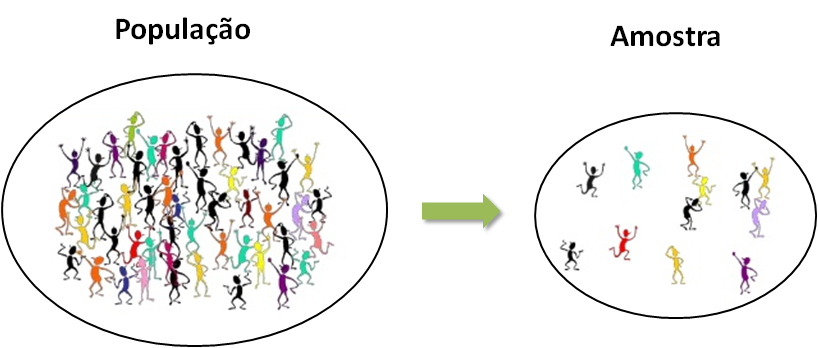
\includegraphics[width=1\linewidth]{figures/esquma_pop_amos} \caption{\label{fig:popamos}Esquema de população e amostra}\label{fig:popAmostra}
\end{figure}

Assim, a motivação de obter uma amostra se deve pela inviabilidade ou até mesmo impossibilidade de se observar toda a população. Como vantagens da amostra, podemos citar: redução de custos, redução de tempo de coleta e reproduz satisfatoriamente a realidade, se a amostra for representativa. A desvantagem se deve pelo motivo desta poder carregar vícios quando feita sem os devidos cuidados.

A técnica considerada para selecionar amostra representativa da população de interesse é a \textbf{amostragem}. A escolha da técnica de amostragem depende de muitas questões e decisões específicas de cada projeto.

Pela experiência em pesquisas na área médica, a definição da técnica de amostragem não é suficiente quando é planejada a coleta da amostra. O que precisa ser definido é o plano amostral.

\begin{quote}
\textbf{Plano amostral:}
Estratégias e especificações metodológicas e estatísticas com o intuito de avaliar a questão científica de maneira adequada.
\end{quote}

No plano amostral, algumas questões precisam ser pensadas:

\begin{itemize}
\item
  Está claramente definida a população de interesse?
\item
  O desenho do estudo é adequado?
\item
  Como será a amostragem?
\item
  O tamanho da amostra é suficiente?
\item
  Estão bem definidas as limitações do estudo?
\item
  O estudo é viável frente a custo, tempo e disponibilidade das unidades?
\item
  Existem variáveis confundidoras?
\item
  Devo pensar em uma análise entre observadores?
\end{itemize}

\hypertarget{variaveis}{%
\section{Variáveis}\label{variaveis}}

Definimos aqui uma variável como sendo uma característica de interesse associada a uma população. Uma variável pode ser classificada em dois tipos:

\begin{itemize}
\item
  \textbf{Qualitativas}: apresentam como possíveis realizações uma qualidade (ou atributo) do indivíduo pesquisado. Exemplos: sexo, grau de instrução, estado civil, classe social, presença de diabetes (sim ou não), etc.
\item
  \textbf{Quantitativas}: apresentam como possíveis realizações números resultantes de uma contagem ou de uma mensuração. Exemplos: Número de filhos, salário, temperatura, pressão arterial, concentração de alguma substância, etc.
\end{itemize}

Ainda, uma \textbf{variável qualitativa} pode ser dividida em \textbf{ordinal} ou \textbf{nominal}, em que:

\begin{itemize}
\item
  \textbf{ordinal}: Existe uma ordem nos seus resultados.
  Exemplo: grau de instrução, estadiamento de uma doença, etc.
\item
  \textbf{nominal}: Não existe nenhuma ordenação nas possíveis realizações.
  Exemplo: Sexo, estado civil, presença de diabetes, etc.
\end{itemize}

Já uma \textbf{variável quantitativa} pode ser dividida em \textbf{discreta} ou \textbf{contínua}, em que:

\begin{itemize}
\tightlist
\item
  \textbf{discreta}: Possíveis valores formam um conjunto finito ou enumerável de pontos e que resultam, frequentemente, de uma contagem. Exemplo:
  número de filhos (0,1,2,\ldots), quantidade de acidentes em um mês (0, 1, 2, \ldots), número de carros que passam no pedágio de Vitória para Vila Velha em 1 hora, etc.
\item
  \textbf{contínua}: Características mensuráveis que assumem valores em um intervalo de números reais. Exemplo: salário, temperatura, pressão arterial, etc.
\end{itemize}

Podemos resumir os tipos de variáveis como o esquema na Figura \ref{fig:tiposVars}.

\begin{figure}
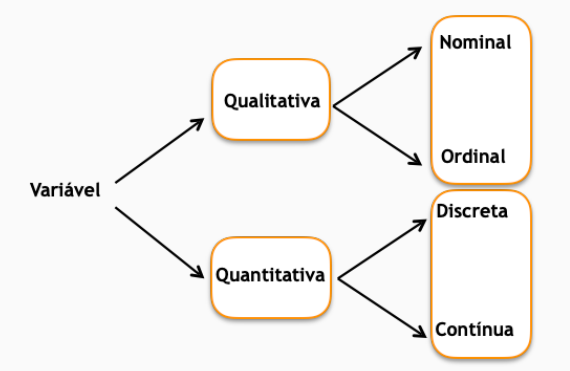
\includegraphics[width=1\linewidth]{figures/tipos_variaveis} \caption{Esquema dos tipos de variáveis}\label{fig:tiposVars}
\end{figure}

A identificação do tipo de variável é importante para a tabulação de dados de maneira correta e também para realizar a análise dos dados de maneira adequada. A seguir falamos sobre a tabulação de dados.

\hypertarget{tabulauxe7uxe3o-de-dados}{%
\section{Tabulação de dados}\label{tabulauxe7uxe3o-de-dados}}

Bases de dados são estruturas organizadas com o objetivo de permitir sua análise estatística. Em geral, cada linha
da planilha corresponde a uma unidade de investigação e cada coluna corresponde a uma variável.

O início dos trabalhos da tabulação dos dados deve ser feito antes da coleta de dados. O planejamento da planilha contribui tanto para o entendimento do processo de coleta de dados quanto para a especificação das variáveis a serem avaliadas. Uma das primeiras medidas é a elaboração de um dicionário com a especificação das variáveis.

Para mais detalhes sobre tabulação de dados, acesse \url{https://daslab-ufes.github.io/materiais/} e clique em ``Tabulacao de Dados''.

\hypertarget{importauxe7uxe3o-de-dados-no-r}{%
\section{Importação de dados no R}\label{importauxe7uxe3o-de-dados-no-r}}

\hypertarget{extensuxe3o-.txt-ou-.csv}{%
\subsection{Extensão .txt ou .csv}\label{extensuxe3o-.txt-ou-.csv}}

Para importar dados para o R, com extensão .txt ou .csv, uma sugestão é utilizar o pacote \texttt{readr}. Como exemplo, consideramos um arquivo chamado dados1 que queremos importar para o R.

\begin{Shaded}
\begin{Highlighting}[]
\KeywordTok{library}\NormalTok{(readr)}
\NormalTok{dados_csv <-}\StringTok{ }\KeywordTok{read_csv}\NormalTok{(}\DataTypeTok{file =} \StringTok{"caminho-para-o-arquivo/dados1.csv"}\NormalTok{)}
\NormalTok{dados_txt <-}\StringTok{ }\KeywordTok{read_delim}\NormalTok{(}\DataTypeTok{file =} \StringTok{"caminho-para-o-arquivo/dados1.txt"}\NormalTok{, }\DataTypeTok{delim =} \StringTok{" "}\NormalTok{)}
\end{Highlighting}
\end{Shaded}

O argumento \texttt{file=} representa o caminho onde o arquivo está alocado. Se o arquivo estiver no diretório de trabalho (quando criamos o projeto e colocamos os arquivos de dados na pasta criada pelo projeto), não precisa especificar o caminho até o arquivo, como segue:

\begin{Shaded}
\begin{Highlighting}[]
\NormalTok{dados_csv <-}\StringTok{ }\KeywordTok{read_csv}\NormalTok{(}\DataTypeTok{file =} \StringTok{"dados1.csv"}\NormalTok{)}
\NormalTok{dados_txt <-}\StringTok{ }\KeywordTok{read_delim}\NormalTok{(}\DataTypeTok{file =} \StringTok{"dados1.txt"}\NormalTok{, }\DataTypeTok{delim =} \StringTok{" "}\NormalTok{)}
\end{Highlighting}
\end{Shaded}

O argumento \texttt{delim=} indica qual o separador das colunas no arquivo de texto.

Outra opção para leitura de arquivo .txt é usar a função \texttt{read.table} que já está salva na base, ou seja, não é necessário instalar pacotes.

\begin{Shaded}
\begin{Highlighting}[]
\NormalTok{dados_txt2 <-}\StringTok{ }\KeywordTok{read.table}\NormalTok{(}\DataTypeTok{file=}\StringTok{"dados1.txt"}\NormalTok{,}\DataTypeTok{header=}\NormalTok{T)}
\end{Highlighting}
\end{Shaded}

O argumento header indica se a primeira linha do arquivo consta o nome das variáveis. Se for T (TRUE), a primeira linha é indicada como nome das variáveis. O \emph{default} (padrão se o usuário não mudar o argumento) é \texttt{header=F}.

Vale ressaltar que para cada função \texttt{read\_}, existe uma respectiva função \texttt{write\_} para salvar o arquivo no formato de interesse. Como exemplo, queremos salvar a base de dados mtcars na pasta do meu computador com o nome cars:

\begin{Shaded}
\begin{Highlighting}[]
\KeywordTok{write_csv}\NormalTok{(}\DataTypeTok{x =}\NormalTok{ mtcars, }\DataTypeTok{path =} \StringTok{"cars.csv"}\NormalTok{)}
\KeywordTok{write_delim}\NormalTok{(}\DataTypeTok{x =}\NormalTok{ mtcars, }\DataTypeTok{delim =} \StringTok{" "}\NormalTok{, }\DataTypeTok{path =} \StringTok{"cars.txt"}\NormalTok{)}\ErrorTok{)}
\end{Highlighting}
\end{Shaded}

\hypertarget{arquivos-em-excel}{%
\subsection{Arquivos em Excel}\label{arquivos-em-excel}}

O pacote \texttt{readxl} pode ser utilizado para leitura de arquivos do Excel, como .xls e xlsx.

\begin{Shaded}
\begin{Highlighting}[]
\KeywordTok{library}\NormalTok{(readxl)}
\NormalTok{dados_excel <-}\StringTok{ }\KeywordTok{read_xls}\NormalTok{(}\DataTypeTok{path =} \StringTok{"dados1.xls"}\NormalTok{) }\CommentTok{#Leitura do arquivo .xls}
\NormalTok{dados_excelx <-}\StringTok{ }\KeywordTok{read_xlsx}\NormalTok{(}\DataTypeTok{path =} \StringTok{"dados1.xlsx"}\NormalTok{) }\CommentTok{#Leitura do arquivo .xlsx}
\end{Highlighting}
\end{Shaded}

Dentre os argumentos dessas funções (veja o \texttt{help()}de cada uma delas), o argumento \texttt{na} indica quais strings (textos) devem ser interpretados como \texttt{NA}. O \emph{default} é considerar espaço em branco no excel.

Uma maneira mais simples é a utilização da função \texttt{read\_excel()}, pois ela auto detecta a extensão do arquivo.

\begin{Shaded}
\begin{Highlighting}[]
\KeywordTok{library}\NormalTok{(readxl)}
\NormalTok{dados_excel1 <-}\StringTok{ }\KeywordTok{read_excel}\NormalTok{(}\DataTypeTok{path =} \StringTok{"dados1.xls"}\NormalTok{)}
\NormalTok{dados_excelx1 <-}\StringTok{ }\KeywordTok{read_excel}\NormalTok{(}\DataTypeTok{path =} \StringTok{"dados1.xlsx"}\NormalTok{)}
\end{Highlighting}
\end{Shaded}

Podemos também exportar um arquivo em excel (.xls e .xlsx) ao considerar a função \texttt{write\_xlsx} do pacote \texttt{writexl}. Suponha que temos o interesse em salvar a base de dados \texttt{dados} em excel na pasta do computador (exportar) com o nome de \texttt{dados\_correto}:

\begin{Shaded}
\begin{Highlighting}[]
\KeywordTok{library}\NormalTok{(writexl)}
\KeywordTok{write_xlsx}\NormalTok{(dados, }\StringTok{"dados_correto.xlsx"}\NormalTok{)}
\end{Highlighting}
\end{Shaded}

\hypertarget{arquivos-de-outros-softwares}{%
\subsection{Arquivos de outros softwares}\label{arquivos-de-outros-softwares}}

Para ler dados salvos em extensão de outros softwares: SPSS, STATA e SAS, podem ser utilizadas as funções do pacote \texttt{haven}.

\begin{Shaded}
\begin{Highlighting}[]
\KeywordTok{library}\NormalTok{(haven)}
\NormalTok{dados_stata <-}\StringTok{ }\KeywordTok{read_stata}\NormalTok{(}\StringTok{"dados1.dta"}\NormalTok{)}
\NormalTok{dados_spss <-}\StringTok{ }\KeywordTok{read_spss}\NormalTok{(}\StringTok{"dados1.sav"}\NormalTok{)}
\NormalTok{dados_sas <-}\StringTok{ }\KeywordTok{read_sas}\NormalTok{(}\StringTok{"dados1.sas7bdat"}\NormalTok{)  }
\end{Highlighting}
\end{Shaded}

Outra opção de pacote para importação de dados de outros softwares é o \texttt{foreign}. Além do SAS, STAT e SPSS, ele também lê dados do Octave, Minitab e Epi Info.

\hypertarget{consistencia}{%
\section{Análise de consistência e tratamento dos dados}\label{consistencia}}

O tratamento dos dados toma muitas vezes a maior parte do tempo de uma análise estatística.

A análise de consistência consiste em realizar uma primeira análise dos dados com o intuito de encontrar inconsistências. São exemplos de inconsistências:

\begin{itemize}
\tightlist
\item
  boas práticas para nome das variáveis.
\item
  como erros de digitação;
\item
  indivíduos imputados mais de uma vez na planilha de dados de maneira errada;
\item
  identificar casos missings e avaliar se a observação está ausente de maneira correta ou não;
\item
  identificar as categorias de variáveis qualitativas.
\end{itemize}

Para exemplificar o que for discutido, consideramos os dados fictícios de \(n=104\) gestações gemelares, apresentado no Capítulo 2. O dicionário contém a explicação das variáveis, a identificação dos valores ausentes de cada variável e o rótulo das categorias de variáveis qualitativas. Uma boa prática na tabulação dos dados é manter o dicionário junto com a base de dados. Se a tabulação for realizada no Excel, por exemplo, manter o dicionário em uma outra aba.

\hypertarget{importauxe7uxe3o-dos-dados}{%
\subsection{Importação dos dados}\label{importauxe7uxe3o-dos-dados}}

\begin{Shaded}
\begin{Highlighting}[]
\KeywordTok{library}\NormalTok{(readxl)}
\NormalTok{dados <-}\StringTok{ }\KeywordTok{read_excel}\NormalTok{(}\DataTypeTok{path =} \StringTok{"dataset/dados_gemelares.xlsx"}\NormalTok{)}
\NormalTok{dados}
\end{Highlighting}
\end{Shaded}

\begin{verbatim}
## # A tibble: 108 x 21
##       ID Grupo CORION `Data aval`         `Data nascimento`   `COR BRANCO`
##    <dbl> <dbl> <chr>  <dttm>              <dttm>                     <dbl>
##  1     1     2 Di     2017-04-23 00:00:00 1988-04-30 00:00:00            1
##  2     2     1 Mono   2016-03-21 00:00:00 1982-03-30 00:00:00            1
##  3     2     1 Mono   2016-03-21 00:00:00 1982-03-30 00:00:00            1
##  4     3     1 Di     2016-02-17 00:00:00 1991-02-23 00:00:00            2
##  5     5     2 Di     2017-04-23 00:00:00 1988-04-30 00:00:00            2
##  6     6     1 Di     2016-03-21 00:00:00 1989-03-28 00:00:00            2
##  7     7     2 Di     2016-02-17 00:00:00 1985-02-24 00:00:00            2
##  8     8     1 Di     2017-12-14 00:00:00 1988-12-21 00:00:00            1
##  9     9     1 Di     2017-04-23 00:00:00 1980-05-02 00:00:00            3
## 10    10     2 Di     2016-03-21 00:00:00 1984-03-29 00:00:00            1
## # ... with 98 more rows, and 15 more variables: `Peso Pré` <dbl>, ALT <dbl>,
## #   Gesta <dbl>, Para <dbl>, Aborto <dbl>, IND_AP <dbl>, Tabagismo <dbl>,
## #   Alcool <dbl>, Drogas <dbl>, IG_Aval <dbl>, MedidaColo <dbl>,
## #   Num_contra_CTG <dbl>, `IGP semana` <dbl>, `IGP dia` <dbl>, oi <lgl>
\end{verbatim}

\textbf{Exercício}: Na base em excel, substitua o espaço em branco (dados faltantes) por NA e rode o seguinte comando:

\begin{Shaded}
\begin{Highlighting}[]
\NormalTok{dados <-}\StringTok{ }\KeywordTok{read_excel}\NormalTok{(}\DataTypeTok{path =} \StringTok{"dataset/dados_gemelares.xlsx"}\NormalTok{,}\DataTypeTok{na=}\StringTok{"NA"}\NormalTok{)}
\end{Highlighting}
\end{Shaded}

O default do missing é o espaço em branco. Acesse o help em ?read\_excel e veja \texttt{na\ =\ ""}.

\hypertarget{arrumauxe7uxe3o-da-base-de-dados}{%
\subsection{Arrumação da base de dados}\label{arrumauxe7uxe3o-da-base-de-dados}}

Inicialmente, vamos verificar os nomes das variáveis na base de dados por meio da função \texttt{names}. Note que os nomes tem letras maiúsculas, espaços e acento. Utilizar os dados com essas características não impossibilita as futuras análises, mas pode atrapalhar quando precisamos selecionar algumas dessas variáveis.

\begin{Shaded}
\begin{Highlighting}[]
\KeywordTok{names}\NormalTok{(dados)}
\end{Highlighting}
\end{Shaded}

\begin{verbatim}
##  [1] "ID"              "Grupo"           "CORION"          "Data aval"      
##  [5] "Data nascimento" "COR BRANCO"      "Peso Pré"        "ALT"            
##  [9] "Gesta"           "Para"            "Aborto"          "IND_AP"         
## [13] "Tabagismo"       "Alcool"          "Drogas"          "IG_Aval"        
## [17] "MedidaColo"      "Num_contra_CTG"  "IGP semana"      "IGP dia"        
## [21] "oi"
\end{verbatim}

uma boa prática consiste em padronizar os nomes das variáveis, até para facilitar a lembrança deles. Para isso, utilizaremos o pacote \texttt{janitor} para a arrumação da base de dados. Usamos a função \texttt{clean\_names()} para primeiro ajuste dos nomes das variáveis.

\begin{Shaded}
\begin{Highlighting}[]
\KeywordTok{library}\NormalTok{(janitor)}
\end{Highlighting}
\end{Shaded}

\begin{Shaded}
\begin{Highlighting}[]
\NormalTok{dados <-}\StringTok{ }\NormalTok{janitor}\OperatorTok{::}\KeywordTok{clean_names}\NormalTok{(dados) }
\end{Highlighting}
\end{Shaded}

Agora vamos ver como ficou o nome das variáveis:

\begin{Shaded}
\begin{Highlighting}[]
\KeywordTok{names}\NormalTok{(dados)}
\end{Highlighting}
\end{Shaded}

\begin{verbatim}
##  [1] "id"              "grupo"           "corion"          "data_aval"      
##  [5] "data_nascimento" "cor_branco"      "peso_pre"        "alt"            
##  [9] "gesta"           "para"            "aborto"          "ind_ap"         
## [13] "tabagismo"       "alcool"          "drogas"          "ig_aval"        
## [17] "medida_colo"     "num_contra_ctg"  "igp_semana"      "igp_dia"        
## [21] "oi"
\end{verbatim}

Veja que ele deixou todos os nomes minúsculos, substituindo o espaço por "\_" e tirando acentos. Isso ajuda a evitar problemas futuros em algumas análises que não lidam muito bem com acentos e espaços nos nomes das variáveis.

Outro problema comum é a presença de linhas e colunas vazias. Na base de dados em questão, não há linhas em branco, como pode ser visto na saída abaixo.

\begin{Shaded}
\begin{Highlighting}[]
\NormalTok{janitor}\OperatorTok{::}\KeywordTok{remove_empty}\NormalTok{(dados,}\StringTok{"rows"}\NormalTok{)}
\end{Highlighting}
\end{Shaded}

\begin{verbatim}
## # A tibble: 108 x 21
##       id grupo corion data_aval           data_nascimento     cor_branco
##    <dbl> <dbl> <chr>  <dttm>              <dttm>                   <dbl>
##  1     1     2 Di     2017-04-23 00:00:00 1988-04-30 00:00:00          1
##  2     2     1 Mono   2016-03-21 00:00:00 1982-03-30 00:00:00          1
##  3     2     1 Mono   2016-03-21 00:00:00 1982-03-30 00:00:00          1
##  4     3     1 Di     2016-02-17 00:00:00 1991-02-23 00:00:00          2
##  5     5     2 Di     2017-04-23 00:00:00 1988-04-30 00:00:00          2
##  6     6     1 Di     2016-03-21 00:00:00 1989-03-28 00:00:00          2
##  7     7     2 Di     2016-02-17 00:00:00 1985-02-24 00:00:00          2
##  8     8     1 Di     2017-12-14 00:00:00 1988-12-21 00:00:00          1
##  9     9     1 Di     2017-04-23 00:00:00 1980-05-02 00:00:00          3
## 10    10     2 Di     2016-03-21 00:00:00 1984-03-29 00:00:00          1
## # ... with 98 more rows, and 15 more variables: peso_pre <dbl>, alt <dbl>,
## #   gesta <dbl>, para <dbl>, aborto <dbl>, ind_ap <dbl>, tabagismo <dbl>,
## #   alcool <dbl>, drogas <dbl>, ig_aval <dbl>, medida_colo <dbl>,
## #   num_contra_ctg <dbl>, igp_semana <dbl>, igp_dia <dbl>, oi <lgl>
\end{verbatim}

Propositalmente, inclui a coluna ``oi'' vazia para podermos eliminá-la com o comando abaixo:

\begin{Shaded}
\begin{Highlighting}[]
\NormalTok{dados <-}\StringTok{ }\NormalTok{janitor}\OperatorTok{::}\KeywordTok{remove_empty}\NormalTok{(dados,}\StringTok{"cols"}\NormalTok{) }\CommentTok{#limpando colunas vazias}
\NormalTok{dados}
\end{Highlighting}
\end{Shaded}

\begin{verbatim}
## # A tibble: 108 x 20
##       id grupo corion data_aval           data_nascimento     cor_branco
##    <dbl> <dbl> <chr>  <dttm>              <dttm>                   <dbl>
##  1     1     2 Di     2017-04-23 00:00:00 1988-04-30 00:00:00          1
##  2     2     1 Mono   2016-03-21 00:00:00 1982-03-30 00:00:00          1
##  3     2     1 Mono   2016-03-21 00:00:00 1982-03-30 00:00:00          1
##  4     3     1 Di     2016-02-17 00:00:00 1991-02-23 00:00:00          2
##  5     5     2 Di     2017-04-23 00:00:00 1988-04-30 00:00:00          2
##  6     6     1 Di     2016-03-21 00:00:00 1989-03-28 00:00:00          2
##  7     7     2 Di     2016-02-17 00:00:00 1985-02-24 00:00:00          2
##  8     8     1 Di     2017-12-14 00:00:00 1988-12-21 00:00:00          1
##  9     9     1 Di     2017-04-23 00:00:00 1980-05-02 00:00:00          3
## 10    10     2 Di     2016-03-21 00:00:00 1984-03-29 00:00:00          1
## # ... with 98 more rows, and 14 more variables: peso_pre <dbl>, alt <dbl>,
## #   gesta <dbl>, para <dbl>, aborto <dbl>, ind_ap <dbl>, tabagismo <dbl>,
## #   alcool <dbl>, drogas <dbl>, ig_aval <dbl>, medida_colo <dbl>,
## #   num_contra_ctg <dbl>, igp_semana <dbl>, igp_dia <dbl>
\end{verbatim}

\hypertarget{identificauxe7uxe3o-de-casos-duplicados}{%
\subsection{Identificação de casos duplicados}\label{identificauxe7uxe3o-de-casos-duplicados}}

Uma boa prática consiste em identificar casos duplicados, isto é, identificar se há casos erroneamente repetidos. No exemplo, a variável chave é ``id'', em que cada indivíduo distinto apresenta um id distinto. Para identificar casos duplicados pela variável chave ``id'', usamos a função \texttt{get\_dupes} do pacote \texttt{janitor}.

\begin{Shaded}
\begin{Highlighting}[]
\NormalTok{janitor}\OperatorTok{::}\KeywordTok{get_dupes}\NormalTok{(dados, id)}
\end{Highlighting}
\end{Shaded}

\begin{verbatim}
## # A tibble: 8 x 21
##      id dupe_count grupo corion data_aval           data_nascimento    
##   <dbl>      <int> <dbl> <chr>  <dttm>              <dttm>             
## 1     2          2     1 Mono   2016-03-21 00:00:00 1982-03-30 00:00:00
## 2     2          2     1 Mono   2016-03-21 00:00:00 1982-03-30 00:00:00
## 3    11          2     2 Di     2016-02-17 00:00:00 1981-02-25 00:00:00
## 4    11          2     2 Di     2016-02-17 00:00:00 1981-02-25 00:00:00
## 5    17          2     1 Di     2017-04-23 00:00:00 1993-04-29 00:00:00
## 6    17          2     1 Di     2017-04-23 00:00:00 1993-04-29 00:00:00
## 7    23          2     2 Di     2016-02-17 00:00:00 1997-02-21 00:00:00
## 8    23          2     2 Di     2016-02-17 00:00:00 1997-02-21 00:00:00
## # ... with 15 more variables: cor_branco <dbl>, peso_pre <dbl>, alt <dbl>,
## #   gesta <dbl>, para <dbl>, aborto <dbl>, ind_ap <dbl>, tabagismo <dbl>,
## #   alcool <dbl>, drogas <dbl>, ig_aval <dbl>, medida_colo <dbl>,
## #   num_contra_ctg <dbl>, igp_semana <dbl>, igp_dia <dbl>
\end{verbatim}

No exemplo, note que os ID's = 2, 11, 17 e 23 aparecem duas vezes cada, o que não está correto para essa aplicação.
Para eliminar linhas duplicadas identificadas, usamos a função \texttt{distinct} do pacote \texttt{dplyr}.

\begin{Shaded}
\begin{Highlighting}[]
\KeywordTok{library}\NormalTok{(dplyr)}
\end{Highlighting}
\end{Shaded}

\begin{Shaded}
\begin{Highlighting}[]
\NormalTok{dados <-}\StringTok{ }\NormalTok{dplyr}\OperatorTok{::}\KeywordTok{distinct}\NormalTok{(dados,id, }\DataTypeTok{.keep_all =} \OtherTok{TRUE}\NormalTok{)}
\NormalTok{dados}
\end{Highlighting}
\end{Shaded}

\begin{verbatim}
## # A tibble: 104 x 20
##       id grupo corion data_aval           data_nascimento     cor_branco
##    <dbl> <dbl> <chr>  <dttm>              <dttm>                   <dbl>
##  1     1     2 Di     2017-04-23 00:00:00 1988-04-30 00:00:00          1
##  2     2     1 Mono   2016-03-21 00:00:00 1982-03-30 00:00:00          1
##  3     3     1 Di     2016-02-17 00:00:00 1991-02-23 00:00:00          2
##  4     5     2 Di     2017-04-23 00:00:00 1988-04-30 00:00:00          2
##  5     6     1 Di     2016-03-21 00:00:00 1989-03-28 00:00:00          2
##  6     7     2 Di     2016-02-17 00:00:00 1985-02-24 00:00:00          2
##  7     8     1 Di     2017-12-14 00:00:00 1988-12-21 00:00:00          1
##  8     9     1 Di     2017-04-23 00:00:00 1980-05-02 00:00:00          3
##  9    10     2 Di     2016-03-21 00:00:00 1984-03-29 00:00:00          1
## 10    11     2 Di     2016-02-17 00:00:00 1981-02-25 00:00:00          1
## # ... with 94 more rows, and 14 more variables: peso_pre <dbl>, alt <dbl>,
## #   gesta <dbl>, para <dbl>, aborto <dbl>, ind_ap <dbl>, tabagismo <dbl>,
## #   alcool <dbl>, drogas <dbl>, ig_aval <dbl>, medida_colo <dbl>,
## #   num_contra_ctg <dbl>, igp_semana <dbl>, igp_dia <dbl>
\end{verbatim}

Ao chamar os dados, apenas as dez primeiras linhas são impressas na tela e as colunas que não couberam na largura do console serão omitidas. Vale ressaltar que, também são apresentadas a dimensão da tabela (no exemplo, 104 X 20) e as classes de cada coluna.

\hypertarget{identificar-problemas-nas-variuxe1veis-da-base-de-dados}{%
\subsection{Identificar problemas nas variáveis da base de dados}\label{identificar-problemas-nas-variuxe1veis-da-base-de-dados}}

Outra etapa importante na análise de consistência é identificar o tipo de variável e ver se o R está interpretando corretamente o tipo de cada variável.

Temos na nossa base de dados colunas de data, além de variáveis qualitativas e quantitativas (veja o dicionário das variáveis na Figura \ref{fig:dic1}). São as variáveis de data: ``data\_aval'' e ``data\_nascimento''. As variáveis qualitativas são: ``grupo'' (progesterona ou placebo), ``corion'' (mono ou dicoriônica), ``cor\_branco'' (branca ou não branca), ``ind\_ap'' (sim ou não), ``tabagismo'' (sim ou não), ``alcool'' (sim ou não) e ``drogas'' (sim ou não). As demais variáveis são quantitativa.

Mas precisamos entender se o R realmente entendeu todas as variáveis da maneira correta. Uma maneira de identificar isso e também de ver algumas descritivas das variáveis que nos auxiliam a ver possíveis inconsistências na base de dados é a a função \texttt{skim} do pacote \texttt{skimr}.

\begin{Shaded}
\begin{Highlighting}[]
\NormalTok{skimr}\OperatorTok{::}\KeywordTok{skim}\NormalTok{(dados)}
\end{Highlighting}
\end{Shaded}

\begin{verbatim}
## Error in kable_latex(x = structure(c("Name", "Number of rows", "Number of columns", : unused argument (table.attr = "style='width: auto;'\n        class='table table-condensed'")
\end{verbatim}

No R, as variáveis qualititativas são nomeadas ``factor'', as variáveis quantitativas são nomeadas ``numeric'' e as variáveis de data são ``date''. Note que na importação dos dados o R não entendeu corretamente os tipos de variáveis. Mas vamos corrigir isso no que segue.

Começando pela data, vamos rodar o seguinte código:

\begin{Shaded}
\begin{Highlighting}[]
\NormalTok{dados}\OperatorTok{$}\NormalTok{data_aval  <-}\StringTok{ }\KeywordTok{as.Date}\NormalTok{(dados}\OperatorTok{$}\NormalTok{data_aval)}
\NormalTok{dados}\OperatorTok{$}\NormalTok{data_nascimento  <-}\StringTok{ }\KeywordTok{as.Date}\NormalTok{(dados}\OperatorTok{$}\NormalTok{data_nascimento)}
\end{Highlighting}
\end{Shaded}

A função \texttt{as.Date} informa para o R que a variável do seu argumento é de data. Vamos ver como ficou:

\begin{Shaded}
\begin{Highlighting}[]
\NormalTok{skimr}\OperatorTok{::}\KeywordTok{skim}\NormalTok{(dados)}
\end{Highlighting}
\end{Shaded}

\begin{verbatim}
## Error in kable_latex(x = structure(c("Name", "Number of rows", "Number of columns", : unused argument (table.attr = "style='width: auto;'\n        class='table table-condensed'")
\end{verbatim}

Agora vamos lidar com as variáveis qualitativas. Veja que ``para''corion" foi identificada como \emph{character}. Isso acontece porque ela foi tabulada como texto. Já as demais variáveis qualitativas estão identificadas como \emph{numeric}, pois na tabulação suas categorias estão codificadas com números. Para então dizer ao R o verdadeiro tipo dessas variáveis, vamos utilizar os seguintes comandos:

\begin{Shaded}
\begin{Highlighting}[]
\NormalTok{  dados}\OperatorTok{$}\NormalTok{grupo <-}\StringTok{ }\KeywordTok{as.factor}\NormalTok{(dados}\OperatorTok{$}\NormalTok{grupo)}
\NormalTok{  dados}\OperatorTok{$}\NormalTok{corion <-}\StringTok{ }\KeywordTok{as.factor}\NormalTok{(dados}\OperatorTok{$}\NormalTok{corion)}
\NormalTok{  dados}\OperatorTok{$}\NormalTok{cor_branco <-}\StringTok{ }\KeywordTok{as.factor}\NormalTok{(dados}\OperatorTok{$}\NormalTok{cor_branco)}
\NormalTok{  dados}\OperatorTok{$}\NormalTok{ind_ap <-}\StringTok{ }\KeywordTok{as.factor}\NormalTok{(dados}\OperatorTok{$}\NormalTok{ind_ap)}
\NormalTok{  dados}\OperatorTok{$}\NormalTok{tabagismo <-}\StringTok{ }\KeywordTok{as.factor}\NormalTok{(dados}\OperatorTok{$}\NormalTok{tabagismo)}
\NormalTok{  dados}\OperatorTok{$}\NormalTok{alcool <-}\StringTok{ }\KeywordTok{as.factor}\NormalTok{(dados}\OperatorTok{$}\NormalTok{alcool)}
\NormalTok{  dados}\OperatorTok{$}\NormalTok{drogas <-}\StringTok{ }\KeywordTok{as.factor}\NormalTok{(dados}\OperatorTok{$}\NormalTok{drogas)}
\end{Highlighting}
\end{Shaded}

A função \texttt{as.factor} é análoga à função \texttt{as.Date}, mas agora informando que as variáveis no argumento da função são qualitativas (factor). Vamos ver como ficou:

\begin{Shaded}
\begin{Highlighting}[]
\NormalTok{skimr}\OperatorTok{::}\KeywordTok{skim}\NormalTok{(dados)}
\end{Highlighting}
\end{Shaded}

\begin{verbatim}
## Error in kable_latex(x = structure(c("Name", "Number of rows", "Number of columns", : unused argument (table.attr = "style='width: auto;'\n        class='table table-condensed'")
\end{verbatim}

Veja que agora as variáveis qualitativas da base estão identificadas no bloco \emph{factor}.

Mas ainda sobre as variáveis qualitativas, podemos identificar algumas inconsistências. Começando pela variável ``cor\_branco'', tem uma categoria 3, o que está errado (1 - branca e 2- não branca). Para poder corrigir essa observação, vamos primeiro identificar quem é esse caso. Para isso, usamos o seguinte comando:

\begin{Shaded}
\begin{Highlighting}[]
\NormalTok{dados[dados}\OperatorTok{$}\NormalTok{cor_branco}\OperatorTok{==}\DecValTok{3}\NormalTok{,]}
\end{Highlighting}
\end{Shaded}

\begin{verbatim}
## # A tibble: 1 x 20
##      id grupo corion data_aval  data_nascimento cor_branco peso_pre   alt gesta
##   <dbl> <fct> <fct>  <date>     <date>          <fct>         <dbl> <dbl> <dbl>
## 1     9 1     Di     2017-04-23 1980-05-02      3                72  1.65     8
## # ... with 11 more variables: para <dbl>, aborto <dbl>, ind_ap <fct>,
## #   tabagismo <fct>, alcool <fct>, drogas <fct>, ig_aval <dbl>,
## #   medida_colo <dbl>, num_contra_ctg <dbl>, igp_semana <dbl>, igp_dia <dbl>
\end{verbatim}

Identificamos que o caso é id=9. O pesquisador viu em seus registros que foi um erro de digitação é o correto é 1 (cor branca). Vamos então corrigir esse ponto na base de dados:

\begin{Shaded}
\begin{Highlighting}[]
\NormalTok{dados}\OperatorTok{$}\NormalTok{cor_branco <-}\StringTok{ }\KeywordTok{ifelse}\NormalTok{(dados}\OperatorTok{$}\NormalTok{id}\OperatorTok{==}\DecValTok{9}\NormalTok{,}\DecValTok{1}\NormalTok{,dados}\OperatorTok{$}\NormalTok{cor_branco)}

\CommentTok{#precisamos informar novamente ao R que cor_branco é fator:}
\NormalTok{dados}\OperatorTok{$}\NormalTok{cor_branco <-}\StringTok{ }\KeywordTok{as.factor}\NormalTok{(dados}\OperatorTok{$}\NormalTok{cor_branco)}
\end{Highlighting}
\end{Shaded}

A função \texttt{ifelse} tem três argumentos. No primeiro, a condição é colocada (no exemplo, se a variável id for igual a 9), o segundo argumento é o que retorna se a condição for verdadeira (no exemplo, se id for realmente igual a 9, a variável ``cor\_branco'' recebe 1) e, por fim, o último argumento é o que retorna se a condição for falsa (se id não for igual a 9 - todas as outras observações da base de dados, a variável ``cor\_branco'' continua com o valor que está).

Outra variável qualitativa com algum problema aparente é ``corion''. Essa variável tem duas categorias: mono e dicoriônica, mas perceba que o R está entendendo que ela tem 4 categorias. Isso acontece porque ela é uma variável de texto (\emph{caracter}) e o R é caso-sensível a letras maiúsculas e minúsculas (o R entende as 4 categorias: Mono, MONO, Di e DI). Por isso, devemos corrigir e deixar todas as respostas ``mono'' escritas da mesma maneira e fazer o mesmo com a categoria ``di''.

Para lidar com variáveis de texto (como é o caso de ``corion''), um pacote no R bastante útil é o \texttt{stringr}. No nosso caso, conseguimos resolver o problema ao colocar todas as palavras em letra minúscula. Para isso, usamos a função \texttt{str\_to\_lower} do pacote \texttt{stringr}:

\begin{Shaded}
\begin{Highlighting}[]
\NormalTok{dados}\OperatorTok{$}\NormalTok{corion <-}\StringTok{ }\NormalTok{stringr}\OperatorTok{::}\KeywordTok{str_to_lower}\NormalTok{(dados}\OperatorTok{$}\NormalTok{corion)}
\end{Highlighting}
\end{Shaded}

Como usei uma função para variáveis de texto, preciso avisar novamente ao R que ``corion'' é fator:

\begin{Shaded}
\begin{Highlighting}[]
\NormalTok{dados}\OperatorTok{$}\NormalTok{corion <-}\StringTok{ }\KeywordTok{as.factor}\NormalTok{(dados}\OperatorTok{$}\NormalTok{corion)}
\end{Highlighting}
\end{Shaded}

Ótimo! Corrigimos as inconsistências das variáveis qualitativas. Mas outra questão surge: como faço para usar um rótulo nos números codificados nas categorias das variáveis qualitativas? Para o grupo, por exemplo, ao invés de aparecer 1 quero que apareça placebo.
Para isso, vamos utilizar o pacote \texttt{forcats} que lida com variáveis qualitativas (categóricas). Para renomear as categorias das variáveis, vamos usar a função \texttt{fct\_recode} desse pacote:

\begin{Shaded}
\begin{Highlighting}[]
\NormalTok{dados}\OperatorTok{$}\NormalTok{grupo <-}\StringTok{ }\NormalTok{forcats}\OperatorTok{::}\KeywordTok{fct_recode}\NormalTok{(dados}\OperatorTok{$}\NormalTok{grupo,}
                                        \DataTypeTok{placebo =} \StringTok{"1"}\NormalTok{,}
                                        \DataTypeTok{progest =} \StringTok{"2"}\NormalTok{)}

\CommentTok{# Agora vamos para a variável cor_branci  (1- branca e 2- nbranca)}
\NormalTok{dados}\OperatorTok{$}\NormalTok{cor_branco <-}\StringTok{ }\NormalTok{forcats}\OperatorTok{::}\KeywordTok{fct_recode}\NormalTok{(dados}\OperatorTok{$}\NormalTok{cor_branco,}
                                \DataTypeTok{branca =} \StringTok{"1"}\NormalTok{,}
                                \DataTypeTok{nbranca =} \StringTok{"2"}\NormalTok{)}

\CommentTok{# Agora vamos para a variável ind_ap (1- sim e 0 -não)}
\NormalTok{dados}\OperatorTok{$}\NormalTok{ind_ap <-}\StringTok{ }\NormalTok{forcats}\OperatorTok{::}\KeywordTok{fct_recode}\NormalTok{(dados}\OperatorTok{$}\NormalTok{ind_ap,}
                                   \DataTypeTok{sim =} \StringTok{"1"}\NormalTok{,}
                                   \DataTypeTok{nao =} \StringTok{"0"}\NormalTok{)}

\CommentTok{# Agora vamos para a variável tabagismo (1- sim e 0 -não)}
\NormalTok{dados}\OperatorTok{$}\NormalTok{tabagismo <-}\StringTok{ }\NormalTok{forcats}\OperatorTok{::}\KeywordTok{fct_recode}\NormalTok{(dados}\OperatorTok{$}\NormalTok{tabagismo,}
                                    \DataTypeTok{sim =} \StringTok{"1"}\NormalTok{,}
                                    \DataTypeTok{nao =} \StringTok{"0"}\NormalTok{)}

\CommentTok{# Agora vamos para a variável alcool  (1- sim e 0 -não)}
\NormalTok{dados}\OperatorTok{$}\NormalTok{alcool  <-}\StringTok{ }\NormalTok{forcats}\OperatorTok{::}\KeywordTok{fct_recode}\NormalTok{(dados}\OperatorTok{$}\NormalTok{alcool,}
                                       \DataTypeTok{sim =} \StringTok{"1"}\NormalTok{,}
                                       \DataTypeTok{nao =} \StringTok{"0"}\NormalTok{)}

\CommentTok{# Agora vamos para a variável drogas  (1- sim e 0 -não)}
\NormalTok{dados}\OperatorTok{$}\NormalTok{drogas  <-}\StringTok{ }\NormalTok{forcats}\OperatorTok{::}\KeywordTok{fct_recode}\NormalTok{(dados}\OperatorTok{$}\NormalTok{drogas,}
                                     \DataTypeTok{sim =} \StringTok{"1"}\NormalTok{,}
                                     \DataTypeTok{nao =} \StringTok{"0"}\NormalTok{)}
\end{Highlighting}
\end{Shaded}

Aqui vale mais uma dica: se você rodar a função \texttt{View(dados)} vai abrir uma janela com a planilha dos dados para visualização. Aparecerá como segue:

\begin{figure}
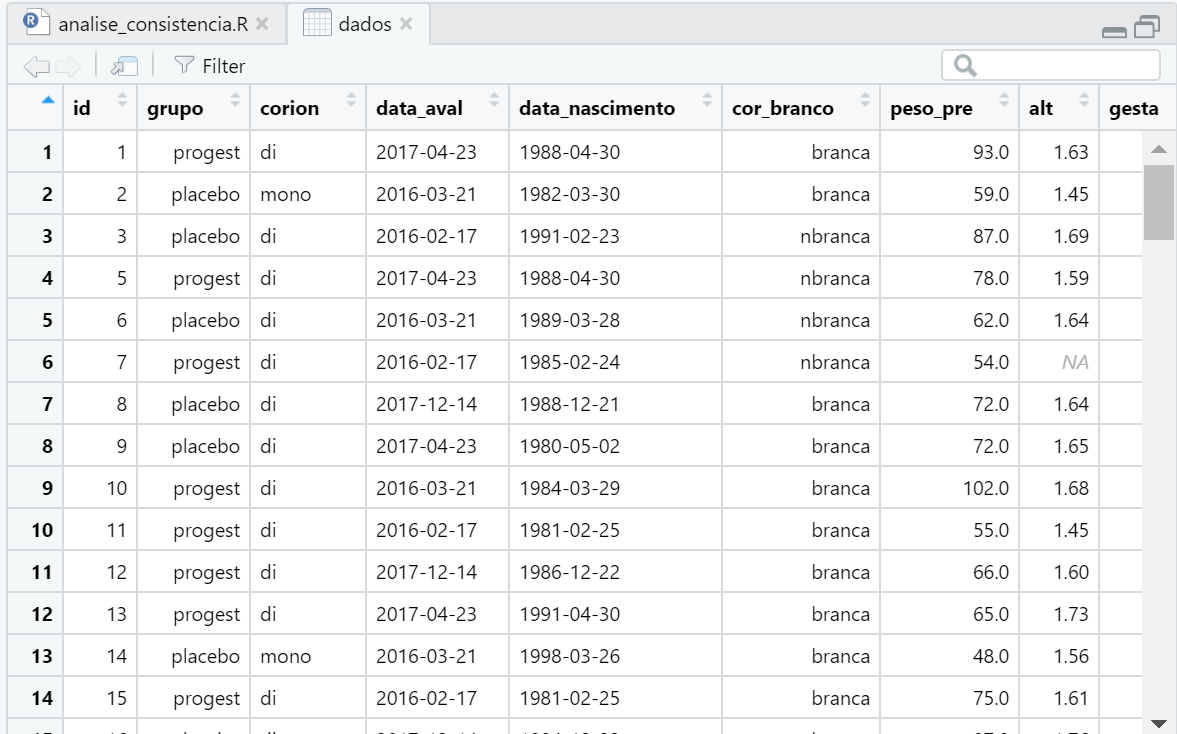
\includegraphics[width=1\linewidth]{figures/print-tela} \caption{Tela dos dados após comando View(dados)}\label{fig:view}
\end{figure}

Finalmente chegamos nas variáveis quantitativas. Uma forma de identificar problemas em variáveis quantitativas é avaliar os valores mínimo e máximo de cada variável e ver se tem algum valor impossível para a mesma.

Veja que tem uma altura de 163. A unidade de medida é em metros e a altura em questão foi um erro de digitação.
O certo era 1.63. Então vamos primeiro identificar o caso e depois vamos corrigir.

\begin{Shaded}
\begin{Highlighting}[]
\NormalTok{dados[dados}\OperatorTok{$}\NormalTok{alt}\OperatorTok{==}\DecValTok{163}\NormalTok{,]}
\end{Highlighting}
\end{Shaded}

\begin{verbatim}
## # A tibble: 3 x 20
##      id grupo corion data_aval  data_nascimento cor_branco peso_pre   alt gesta
##   <dbl> <fct> <fct>  <date>     <date>          <fct>         <dbl> <dbl> <dbl>
## 1    NA <NA>  <NA>   NA         NA              <NA>             NA    NA    NA
## 2    27 prog~ di     2016-02-17 1997-02-21      nbranca          58   163     1
## 3    NA <NA>  <NA>   NA         NA              <NA>             NA    NA    NA
## # ... with 11 more variables: para <dbl>, aborto <dbl>, ind_ap <fct>,
## #   tabagismo <fct>, alcool <fct>, drogas <fct>, ig_aval <dbl>,
## #   medida_colo <dbl>, num_contra_ctg <dbl>, igp_semana <dbl>, igp_dia <dbl>
\end{verbatim}

O caso em questão é o id=27 e vamos novamente usar a função \texttt{ifelse} para substituir o valorr:

\begin{Shaded}
\begin{Highlighting}[]
\NormalTok{dados}\OperatorTok{$}\NormalTok{alt <-}\StringTok{ }\KeywordTok{ifelse}\NormalTok{(dados}\OperatorTok{$}\NormalTok{id}\OperatorTok{==}\DecValTok{27}\NormalTok{,}\FloatTok{1.63}\NormalTok{,dados}\OperatorTok{$}\NormalTok{alt)}
\end{Highlighting}
\end{Shaded}

Há também um valor absurdo para ``ig\_aval'' (idade gestacional da avalição) de 83.86. Vamos identificar o id para depois corrigir:

\begin{Shaded}
\begin{Highlighting}[]
\NormalTok{dados[dados}\OperatorTok{$}\NormalTok{ig_aval}\OperatorTok{==}\FloatTok{83.86}\NormalTok{,]}
\end{Highlighting}
\end{Shaded}

\begin{verbatim}
## # A tibble: 1 x 20
##      id grupo corion data_aval  data_nascimento cor_branco peso_pre   alt gesta
##   <dbl> <fct> <fct>  <date>     <date>          <fct>         <dbl> <dbl> <dbl>
## 1    21 plac~ mono   2017-04-23 1988-04-30      branca           44  1.64     1
## # ... with 11 more variables: para <dbl>, aborto <dbl>, ind_ap <fct>,
## #   tabagismo <fct>, alcool <fct>, drogas <fct>, ig_aval <dbl>,
## #   medida_colo <dbl>, num_contra_ctg <dbl>, igp_semana <dbl>, igp_dia <dbl>
\end{verbatim}

Como podemos observar, o id=21 é o caso inconsistente para ``ig\_aval'' e o pesquisador checou que o correto é 33.86. Vamos então corrigir novamente com a função \texttt{ifelse}.

\begin{Shaded}
\begin{Highlighting}[]
\NormalTok{dados}\OperatorTok{$}\NormalTok{ig_aval <-}\StringTok{ }\KeywordTok{ifelse}\NormalTok{(dados}\OperatorTok{$}\NormalTok{id}\OperatorTok{==}\DecValTok{21}\NormalTok{,}\FloatTok{33.86}\NormalTok{,dados}\OperatorTok{$}\NormalTok{ig_aval)}
\end{Highlighting}
\end{Shaded}

Agora está tudo certo?

\begin{Shaded}
\begin{Highlighting}[]
\NormalTok{skimr}\OperatorTok{::}\KeywordTok{skim}\NormalTok{(dados)}
\end{Highlighting}
\end{Shaded}

\begin{verbatim}
## Error in kable_latex(x = structure(c("Name", "Number of rows", "Number of columns", : unused argument (table.attr = "style='width: auto;'\n        class='table table-condensed'")
\end{verbatim}

\hypertarget{transformauxe7uxe3o-dos-dados}{%
\section{Transformação dos dados}\label{transformauxe7uxe3o-dos-dados}}

Nessa parte do material discutiremos como fazer algumas transformações úteis nas variáveis. Para isso, utilizaremos as funções do pacote \texttt{dplyr}, um pacote bastante útil para a manipulação de dados.

\hypertarget{transformauxe7uxe3o-de-variuxe1veis-quantitativas}{%
\subsection{Transformação de variáveis quantitativas}\label{transformauxe7uxe3o-de-variuxe1veis-quantitativas}}

Primeiramente, temos o interesse em criar a variável IMC, dada pelo peso (em kg) dividido pela altura (em metros) ao quadrado. Para isso, usamos a função \texttt{mutate} do \texttt{dplyr}:

\begin{Shaded}
\begin{Highlighting}[]
\NormalTok{dados <-}\StringTok{ }\NormalTok{dplyr}\OperatorTok{::}\KeywordTok{mutate}\NormalTok{(dados,}\DataTypeTok{imc =}\NormalTok{ peso_pre}\OperatorTok{/}\NormalTok{(alt}\OperatorTok{^}\DecValTok{2}\NormalTok{))}
\end{Highlighting}
\end{Shaded}

Vamos ver então como ficou:

\begin{Shaded}
\begin{Highlighting}[]
\NormalTok{skimr}\OperatorTok{::}\KeywordTok{skim}\NormalTok{(dados}\OperatorTok{$}\NormalTok{imc) }\CommentTok{#coloquei só imc para só fazer descritivas para imc.}
\end{Highlighting}
\end{Shaded}

\begin{verbatim}
## Error in kable_latex(x = structure(c("Name", "Number of rows", "Number of columns", : unused argument (table.attr = "style='width: auto;'\n        class='table table-condensed'")
\end{verbatim}

Note que há três valores ausentes para ``imc'', uma vez que há dois valores ausentes para ``alt'' e outro para ``peso\_pre''.

Observe que na planilha tem duas colunas sobre idade gestacional: igp\_semanas (idade gestacional em semanas fechadas) e igp\_dia (dias ainda não de 1 semana completa). Vamos criar uma coluna que combine essas duas informações e que transforme os dias em semanas de maneira fracionada.

\begin{Shaded}
\begin{Highlighting}[]
\NormalTok{dados <-}\StringTok{ }\NormalTok{dplyr}\OperatorTok{::}\KeywordTok{mutate}\NormalTok{(dados,}\DataTypeTok{igp =}\NormalTok{ igp_semana}\OperatorTok{+}\NormalTok{igp_dia}\OperatorTok{/}\DecValTok{7}\NormalTok{)}
\end{Highlighting}
\end{Shaded}

Vamos ver então como ficou:

\begin{Shaded}
\begin{Highlighting}[]
\NormalTok{skimr}\OperatorTok{::}\KeywordTok{skim}\NormalTok{(dados}\OperatorTok{$}\NormalTok{igp) }\CommentTok{#coloquei só igp para só fazer descritivas para igp.}
\end{Highlighting}
\end{Shaded}

\begin{verbatim}
## Error in kable_latex(x = structure(c("Name", "Number of rows", "Number of columns", : unused argument (table.attr = "style='width: auto;'\n        class='table table-condensed'")
\end{verbatim}

\hypertarget{transformauxe7uxe3o-de-variuxe1veis-qualitativas}{%
\subsection{Transformação de variáveis qualitativas}\label{transformauxe7uxe3o-de-variuxe1veis-qualitativas}}

A variável ``gesta'' indica o número de gestações, contando com a atual da gestante em gestão. Logo, uma gestante com gesta=1 está em sua primeira gestação, ou seja, é primigesta. Queremos criar uma nova variável indicadora de gestação primigesta. Há diferentes forma de fazer isso. Vamos usar o comando \texttt{ifelse} já utilizado anteriormente:

\begin{Shaded}
\begin{Highlighting}[]
\NormalTok{dados}\OperatorTok{$}\NormalTok{primigesta <-}\StringTok{ }\KeywordTok{ifelse}\NormalTok{(dados}\OperatorTok{$}\NormalTok{gesta}\OperatorTok{==}\DecValTok{1}\NormalTok{,}\DecValTok{1}\NormalTok{,}\DecValTok{0}\NormalTok{)}
\end{Highlighting}
\end{Shaded}

Agora vamos recodificar primigesta com o nome de cada categoria:

\begin{Shaded}
\begin{Highlighting}[]
\NormalTok{dados}\OperatorTok{$}\NormalTok{primigesta <-}\StringTok{ }\KeywordTok{as.factor}\NormalTok{(dados}\OperatorTok{$}\NormalTok{primigesta)}
\NormalTok{dados}\OperatorTok{$}\NormalTok{primigesta <-}\StringTok{ }\NormalTok{forcats}\OperatorTok{::}\KeywordTok{fct_recode}\NormalTok{(dados}\OperatorTok{$}\NormalTok{primigesta,}
                                \DataTypeTok{nao =} \StringTok{"0"}\NormalTok{, }
                                \DataTypeTok{sim =} \StringTok{"1"}\NormalTok{)}
\end{Highlighting}
\end{Shaded}

Outra variável qualitativa que é função de uma variável quantitativa da planilha é a prematuridade. Definimos aqui prematuridade se idade gestacional do parto for menor que 37 semanas.

\begin{Shaded}
\begin{Highlighting}[]
\NormalTok{dados}\OperatorTok{$}\NormalTok{prematuridade <-}\StringTok{ }\KeywordTok{ifelse}\NormalTok{(dados}\OperatorTok{$}\NormalTok{igp}\OperatorTok{<}\DecValTok{37}\NormalTok{,}\DecValTok{1}\NormalTok{,}\DecValTok{0}\NormalTok{)}
\end{Highlighting}
\end{Shaded}

Agora vamos recodificar ``prematuridade'' com o nome de cada categoria:

\begin{Shaded}
\begin{Highlighting}[]
\NormalTok{dados}\OperatorTok{$}\NormalTok{prematuridade <-}\StringTok{ }\KeywordTok{as.factor}\NormalTok{(dados}\OperatorTok{$}\NormalTok{prematuridade)}
\NormalTok{dados}\OperatorTok{$}\NormalTok{prematuridade <-}\StringTok{ }\NormalTok{forcats}\OperatorTok{::}\KeywordTok{fct_recode}\NormalTok{(dados}\OperatorTok{$}\NormalTok{prematuridade,}
                                \DataTypeTok{nao =} \StringTok{"0"}\NormalTok{, }
                                \DataTypeTok{sim =} \StringTok{"1"}\NormalTok{)}
\end{Highlighting}
\end{Shaded}

Vamos ver então como ficou:

\begin{Shaded}
\begin{Highlighting}[]
\NormalTok{skimr}\OperatorTok{::}\KeywordTok{skim}\NormalTok{(dados,primigesta,prematuridade) }
\end{Highlighting}
\end{Shaded}

\begin{verbatim}
## Error in kable_latex(x = structure(c("Name", "Number of rows", "Number of columns", : unused argument (table.attr = "style='width: auto;'\n        class='table table-condensed'")
\end{verbatim}

Veja que coloquei ``primigesta'' e ``prematuridade'' no segundo e terceiro argumento do \texttt{skim}para apenas retornar as descritivas dessas duas variáveis.

\textbf{Exercício}:

\begin{enumerate}
\def\labelenumi{\arabic{enumi})}
\item
  Crie a variável indicador\_aborto (sim e nao) - sim se aborto \textgreater=1 e nao se aborto=0.
\item
  Crie a variável primipara (sim e nao) - sim se para \textgreater=1 e nao se para=0.
\end{enumerate}

\hypertarget{manipulauxe7uxe3o-de-datas}{%
\subsection{Manipulação de datas}\label{manipulauxe7uxe3o-de-datas}}

Na base de dados, há duas variáveis de data: data da avaliação e data do nascimento. A diferença entre as duas datas, em anos, é a idade da gestante no momento da avaliação. Para realizar operações com data, usaremos o pacote \texttt{lubridate}.

A data está salva no formato ano-mês-dia e por isso usamos a função \texttt{ymd(.)} para as variáveis de data. Para calcular a diferença entre as data, usamos a função \(%--%
\), atribuindo ao objeto intervalo. Por fim, obtemos a idade ao dividir o intervalo por ano.

\begin{Shaded}
\begin{Highlighting}[]
\NormalTok{intervalo <-}\StringTok{ }\NormalTok{lubridate}\OperatorTok{::}\KeywordTok{ymd}\NormalTok{(dados}\OperatorTok{$}\NormalTok{data_nascimento)}\OperatorTok\StringTok{  }\NormalTok{lubridate}\OperatorTok{::}\KeywordTok{ymd}\NormalTok{(dados}\OperatorTok{$}\NormalTok{data_aval)}
\NormalTok{dados}\OperatorTok{$}\NormalTok{idade <-}\StringTok{ }\NormalTok{intervalo }\OperatorTok{/}\StringTok{ }\NormalTok{lubridate}\OperatorTok{::}\KeywordTok{dyears}\NormalTok{(}\DecValTok{1}\NormalTok{)  }\CommentTok{#número de anos}
\NormalTok{dados}\OperatorTok{$}\NormalTok{idade <-}\StringTok{ }\KeywordTok{trunc}\NormalTok{(dados}\OperatorTok{$}\NormalTok{idade) }\CommentTok{#usamos a idade completada }
\end{Highlighting}
\end{Shaded}

A última linha do código acima utiliza a função \texttt{trunc} para truncar a idade para não usar a fração dos meses da idade ainda não completa e sim usar a idade completada no último aniversário.

Vale ressaltar que há várias funções importantes para lidar com variáveis de data no pacote \texttt{lubridate}. Para mais detalhes, ver a \href{https://cran.r-project.org/web/packages/lubridate/vignettes/lubridate.html}{documentação do lubridate}.

\hypertarget{filtragem-de-observauxe7uxf5es}{%
\subsection{Filtragem de observações}\label{filtragem-de-observauxe7uxf5es}}

Uma função bastante importante quando estamos analisando dados é filtrar de acordo com uma condição de interesse. Suponha que temos interesse em realizar uma determinada análise apenas com gestantes com menos de 23 anos. Para selecionar apenas as gestantes mais novas, podemos utilizar a função \texttt{filter} do pacote \texttt{dplyr}.

\begin{Shaded}
\begin{Highlighting}[]
\NormalTok{dados_jovens <-}\StringTok{ }\KeywordTok{filter}\NormalTok{(dados,idade}\OperatorTok{<}\DecValTok{23}\NormalTok{)}
\end{Highlighting}
\end{Shaded}

Veja que agora o objeto dados\_jovens é a base de dados apenas com aquelas cuja idade é menor que 23 (use o comando View(dados\_jovens) para verificar).

Utilizando os operadores lógicos ``\&'' (e) e ``\textbar{}'' (ou), conseguimos realizar algumas condições, como mostrado no exemplo abaixo.

Agora, queremos selecionar apenas as gestantes mais novas e do grupo progesterona. Para isso:

\begin{Shaded}
\begin{Highlighting}[]
\NormalTok{dados_jovens_progest <-}\StringTok{  }\KeywordTok{filter}\NormalTok{(dados,idade}\OperatorTok{<}\DecValTok{23} \OperatorTok{&}\StringTok{ }\NormalTok{grupo}\OperatorTok{==}\StringTok{"progest"}\NormalTok{)}
\end{Highlighting}
\end{Shaded}

Acho que aqui vale uma nota sobre o pacote \texttt{dplyr} e por isso dediquei uma subseção para ele, no que segue.

\hypertarget{pacote-dplyr}{%
\subsubsection{Pacote dplyr}\label{pacote-dplyr}}

O \texttt{\{dplyr\}} é um pacote muito útil para realizar transformação de dados.

Suas principais funções são:

\begin{itemize}
\item
  filter() - filtra linhas;
\item
  select() - seleciona colunas;
\item
  arrange() - ordena a base;
\item
  mutate() - cria/modifica colunas.
\end{itemize}

Já falamos das funções \texttt{filter} e \texttt{mutate} anteriormente, então falamos brevemente das outras funções no que segue.

A função \texttt{select()} seleciona colunas (variáveis). Vamos supor que eu tenha interesse em criar um objeto com só as variáveis ``id'', ``grupo'', ``prematuridade''.

\begin{Shaded}
\begin{Highlighting}[]
\NormalTok{dados_s <-}\StringTok{ }\NormalTok{dplyr}\OperatorTok{::}\KeywordTok{select}\NormalTok{(dados,id, grupo, prematuridade)}
\end{Highlighting}
\end{Shaded}

Veja em \texttt{View(dados\_s)} que essa base de dados só contém as colunas selecionadas.

Sempre quando queremos retirar algo do banco de dados, colocamos um ``-'' antes da variável. No exemplo abaixo, queremos rerirar ``igp\_semana'' e ``igp\_dia''.

\begin{Shaded}
\begin{Highlighting}[]
\NormalTok{dados_s1 <-}\StringTok{ }\NormalTok{dplyr}\OperatorTok{::}\KeywordTok{select}\NormalTok{(dados,}\OperatorTok{-}\NormalTok{igp_semana,}\OperatorTok{-}\NormalTok{igp_dia)}
\end{Highlighting}
\end{Shaded}

Veja em \texttt{View(dados\_s1)} que essa base de dados só contém as colunas selecionadas.

Com a função \texttt{arrange()}, conseguimos ordenar a base de acordo com uma ou mais colunas. Para gerar uma ordem descescente de alguma variável, utilizamos a função \texttt{desc} como segue:

\begin{Shaded}
\begin{Highlighting}[]
\NormalTok{dados_cres <-}\StringTok{ }\NormalTok{dplyr}\OperatorTok{::}\KeywordTok{arrange}\NormalTok{(dados,alt)}
\end{Highlighting}
\end{Shaded}

\begin{Shaded}
\begin{Highlighting}[]
\NormalTok{dados_decres <-}\StringTok{ }\NormalTok{dplyr}\OperatorTok{::}\KeywordTok{arrange}\NormalTok{(dados,}\KeywordTok{desc}\NormalTok{(alt))}
\end{Highlighting}
\end{Shaded}

No primeiro código acima, ordenamos a planilha em ordem crescente pela altura. Já no segundo código, ordenamos a planilha em ordem decrescente pela altura (a primeira observação na planilha dados\_decres é aquela cuja gestante é a mais alta).

\hypertarget{manipulando-os-formatos-das-bases-de-dados}{%
\section{Manipulando os formatos das bases de dados}\label{manipulando-os-formatos-das-bases-de-dados}}

\hypertarget{combinando-bases-de-dados}{%
\subsection{Combinando bases de dados}\label{combinando-bases-de-dados}}

Vamos considerar que temos interesse em juntar as bases de dados ``dados\_gemelares'' e ``dados\_gemelares\_2''. As duas bases apresentam os mesmos indivíduos (linhas), mas com variáveis (colunas) diferentes.

Vamos então ler a base de dados, atribuindo para o objeto ``dados2''.

\begin{Shaded}
\begin{Highlighting}[]
\KeywordTok{library}\NormalTok{(readxl)}
\NormalTok{dados2 <-}\StringTok{ }\KeywordTok{read_excel}\NormalTok{(}\DataTypeTok{path =} \StringTok{"dataset/dados_gemelares_2.xlsx"}\NormalTok{)}

\NormalTok{dados2}
\end{Highlighting}
\end{Shaded}

\begin{verbatim}
## # A tibble: 104 x 7
##       ID EPDS_antes EPDS_depois EDPS_antes_SN EDPS_depois_SN Grupo_amamentac~
##    <dbl>      <dbl>       <dbl>         <dbl>          <dbl>            <dbl>
##  1     1         20          22             1              1                3
##  2     2         20          24             1              1                1
##  3     3          7           6             0              0                2
##  4     5         10          11             0              0                1
##  5     6          5          20             0              1                2
##  6     7          2           3             0              0                1
##  7     8         12          16             1              1                3
##  8     9         10          16             0              1                3
##  9    10          1           4             0              0                3
## 10    11         10          12             0              1                3
## # ... with 94 more rows, and 1 more variable: Tempo_amamentacao_meses <dbl>
\end{verbatim}

Há algumas funções de combinação de duas bases de dados no pacote \texttt{dplyr}. Elas recebem três argumentos: a primeira base a ser declarada \texttt{(x=)}, a segunda base a ser declarada \texttt{(y=)} e a variável de identificação informada no argumento \texttt{by=}. Aqui estão as funções mais úteis:

\begin{itemize}
\item
  \texttt{left\_join()} - retorna todas as linhas da base de dados no argumento \texttt{x} e todas as colunas das duas bases de dados. Linhas da base de dados de \texttt{x} sem correspondentes em \texttt{y} receberão \texttt{NA} na base de dados combinada.
\item
  \texttt{right\_join()} - retorna todas as linhas da base de dados no argumento \texttt{y} e todas as colunas das duas bases de dados. Linhas da base de dados de \texttt{y} sem correspondentes em \texttt{x} receberão \texttt{NA} na base de dados combinada.
\item
  \texttt{full\_join()} - retorna todas as linhas e todas as colunas de \texttt{x} e de \texttt{y}. As linhas sem correspondência entre as bases receberão \texttt{NA} na base de dados combinada.
\item
  \texttt{inner\_join()} - filtra a base de dados no argumento \texttt{x} apenas onde tem valores correspondentes na base de dados no argumento \texttt{y} e todas as colunas das duas bases de dados.
\item
  \texttt{semi\_join()} - filtra a base de dados no argumento \texttt{x} apenas onde tem valores correspondentes na base de dados no argumento \texttt{y}, mantendo apenas as colunas da base de dados de \texttt{x}.
\item
  \texttt{anti\_join()} - filtra a base de dados no argumento \texttt{x} para incluir apenas valores que \textbf{não possuem} correspondências na base de dados no argumento \texttt{y}.
\end{itemize}

Assim sendo, no nosso exemplo, tanto as funções \texttt{left\_join()}, \texttt{right\_join()}, \texttt{full\_join()} e \texttt{inner\_join()} retornarão a mesma combinação, pois ``dados'' e ``dados2'' possuem exatamente os mesmos indivíduos, ou seja, não há nenhuma linha que esteja em uma das bases de dados e que não está na outra.

\begin{Shaded}
\begin{Highlighting}[]
\NormalTok{dados_todos <-}\StringTok{ }\KeywordTok{full_join}\NormalTok{(dados, dados2, }\DataTypeTok{by=}\KeywordTok{c}\NormalTok{(}\StringTok{"id"}\NormalTok{ =}\StringTok{ "ID"}\NormalTok{)) }
\CommentTok{#faço c("id" = "ID") porque id está em dados e ID (maiúsculo) está em dados2.}

\KeywordTok{str}\NormalTok{(dados_todos)}
\end{Highlighting}
\end{Shaded}

\begin{verbatim}
## tibble [104 x 31] (S3: tbl_df/tbl/data.frame)
##  $ id                     : num [1:104] 1 2 3 5 6 7 8 9 10 11 ...
##  $ grupo                  : Factor w/ 2 levels "placebo","progest": 2 1 1 2 1 2 1 1 2 2 ...
##  $ corion                 : Factor w/ 2 levels "di","mono": 1 2 1 1 1 1 1 1 1 1 ...
##  $ data_aval              : Date[1:104], format: "2017-04-23" "2016-03-21" ...
##  $ data_nascimento        : Date[1:104], format: "1988-04-30" "1982-03-30" ...
##  $ cor_branco             : Factor w/ 2 levels "branca","nbranca": 1 1 2 2 2 2 1 1 1 1 ...
##  $ peso_pre               : num [1:104] 93 59 87 78 62 54 72 72 102 55 ...
##  $ alt                    : num [1:104] 1.63 1.45 1.69 1.59 1.64 NA 1.64 1.65 1.68 1.45 ...
##  $ gesta                  : num [1:104] 3 3 2 7 7 2 2 8 3 1 ...
##  $ para                   : num [1:104] 1 1 1 2 4 1 1 4 2 0 ...
##  $ aborto                 : num [1:104] 1 1 0 4 2 0 0 3 0 0 ...
##  $ ind_ap                 : Factor w/ 2 levels "nao","sim": 1 1 1 1 2 1 1 1 1 2 ...
##  $ tabagismo              : Factor w/ 2 levels "nao","sim": 1 1 1 2 1 1 2 1 1 2 ...
##  $ alcool                 : Factor w/ 2 levels "nao","sim": 1 1 1 2 1 1 1 1 1 2 ...
##  $ drogas                 : Factor w/ 2 levels "nao","sim": 1 1 1 1 1 1 1 1 1 1 ...
##  $ ig_aval                : num [1:104] 33.7 33.4 30.9 32.9 28.4 ...
##  $ medida_colo            : num [1:104] 33 34.6 25 32.8 20.6 33.1 28 21.8 46.3 36 ...
##  $ num_contra_ctg         : num [1:104] 9 4 5 5 2 1 3 2 8 2 ...
##  $ igp_semana             : num [1:104] 37 37 35 38 29 38 34 36 37 33 ...
##  $ igp_dia                : num [1:104] 4 3 0 3 3 3 6 3 5 3 ...
##  $ imc                    : num [1:104] 35 28.1 30.5 30.9 23.1 ...
##  $ igp                    : num [1:104] 37.6 37.4 35 38.4 29.4 ...
##  $ primigesta             : Factor w/ 2 levels "nao","sim": 1 1 1 1 1 1 1 1 1 2 ...
##  $ prematuridade          : Factor w/ 2 levels "nao","sim": 1 1 2 1 2 1 2 2 1 2 ...
##  $ idade                  : num [1:104] 28 33 24 28 26 30 28 36 31 34 ...
##  $ EPDS_antes             : num [1:104] 20 20 7 10 5 2 12 10 1 10 ...
##  $ EPDS_depois            : num [1:104] 22 24 6 11 20 3 16 16 4 12 ...
##  $ EDPS_antes_SN          : num [1:104] 1 1 0 0 0 0 1 0 0 0 ...
##  $ EDPS_depois_SN         : num [1:104] 1 1 0 0 1 0 1 1 0 1 ...
##  $ Grupo_amamentacao      : num [1:104] 3 1 2 1 2 1 3 3 3 3 ...
##  $ Tempo_amamentacao_meses: num [1:104] 8 17 3 11 14 13 8 11 9 4 ...
\end{verbatim}

\hypertarget{formato}{%
\subsection{Mudando formato da base de dado}\label{formato}}

Considere a base de dados abaixo. Veja que ela está no formato \emph{long}, em que as avaliações do mesmo indivíduo (variável de identificação de indivíduo é ``registro'') estão nas linhas.

\begin{figure}
\includegraphics[width=1\linewidth]{figures/dados_exemplo} \caption{Variáveis da base de dados gestações gemelares.}\label{fig:unnamed-chunk-125}
\end{figure}

Primeiro vamos ler a base de dados e atribuí-la ao objeto ``dadosa'':

\begin{Shaded}
\begin{Highlighting}[]
\NormalTok{dadosa <-}\StringTok{ }\KeywordTok{read_excel}\NormalTok{(}\DataTypeTok{path =} \StringTok{"dataset/dados_exemplo.xlsx"}\NormalTok{)}
\end{Highlighting}
\end{Shaded}

Queremos que as avaliações fiquem nas colunas, com as três colunas: aval1, aval2, aval3, ou seja, queremos o formato \emph{wide}. Um pacote do R que pode nos auxiliar a transformar formato \emph{long} em \emph{wide} e vice-versa é o \texttt{tidyr}. A função que usaremos é \texttt{spread}, como segue:

\begin{Shaded}
\begin{Highlighting}[]
\KeywordTok{library}\NormalTok{(tidyr)}
\NormalTok{dadosa1 <-}\StringTok{ }\KeywordTok{spread}\NormalTok{(}\DataTypeTok{data=}\NormalTok{dadosa, }\DataTypeTok{key =}\NormalTok{ avaliacao,}\DataTypeTok{value =}\NormalTok{ peso_fetal)}
\NormalTok{dadosa1}
\end{Highlighting}
\end{Shaded}

\begin{verbatim}
## # A tibble: 5 x 5
##   registro grupo    aval1 aval2 aval3
##      <dbl> <chr>    <dbl> <dbl> <dbl>
## 1        1 caso       500   800  1300
## 2        2 controle   670   990  1470
## 3        3 caso       600   730  1200
## 4        4 caso       700   930  1580
## 5        5 controle   640   890  1500
\end{verbatim}

Agora, se o interesse for transformar o formato \emph{wide} para \emph{long}, a função do \texttt{tidyr} é \texttt{gather}. Vamos ver como fica:

\begin{Shaded}
\begin{Highlighting}[]
\NormalTok{dadosa2 <-}\StringTok{  }\KeywordTok{gather}\NormalTok{(}\DataTypeTok{data=}\NormalTok{dadosa1, }\DataTypeTok{key =}\StringTok{"avaliacao"}\NormalTok{, }\DataTypeTok{value =} \StringTok{"peso_feto"}\NormalTok{, aval1, aval2, aval3)}
\NormalTok{dadosa2}
\end{Highlighting}
\end{Shaded}

\begin{verbatim}
## # A tibble: 15 x 4
##    registro grupo    avaliacao peso_feto
##       <dbl> <chr>    <chr>         <dbl>
##  1        1 caso     aval1           500
##  2        2 controle aval1           670
##  3        3 caso     aval1           600
##  4        4 caso     aval1           700
##  5        5 controle aval1           640
##  6        1 caso     aval2           800
##  7        2 controle aval2           990
##  8        3 caso     aval2           730
##  9        4 caso     aval2           930
## 10        5 controle aval2           890
## 11        1 caso     aval3          1300
## 12        2 controle aval3          1470
## 13        3 caso     aval3          1200
## 14        4 caso     aval3          1580
## 15        5 controle aval3          1500
\end{verbatim}

\hypertarget{exercuxedcios}{%
\section{Exercícios}\label{exercuxedcios}}

\hypertarget{teuxf3ricos}{%
\subsection{Teóricos}\label{teuxf3ricos}}

\begin{enumerate}
\def\labelenumi{\arabic{enumi}.}
\item
  Por que é importante ter a população bem definida?
\item
  Por que é importante pensar em todo planejamento amostral ao
  invés de pensar apenas no cálculo do tamanho amostral?
\item
  O que é uma variável confundidora?
\item
  Classifique as seguintes variáveis:
\end{enumerate}

\begin{enumerate}
\def\labelenumi{\alph{enumi}.}
\item
  Sexo
\item
  Altura
\item
  Peso
\item
  Fuma (sim ou não)
\item
  Tolerância ao cigarro (indiferente, incomoda pouco, incomoda muito)
\item
  Consumo de café (nunca, 1 a 2 vezes por semana, 3 a 6 vezes por semana, uma vez por dia, \(>\) 1 vez por dia)
\item
  Horas de atividade física por semana
\end{enumerate}

\hypertarget{pruxe1ticos-no-r}{%
\subsection{Práticos no R}\label{pruxe1ticos-no-r}}

\begin{enumerate}
\def\labelenumi{\arabic{enumi}.}
\setcounter{enumi}{4}
\tightlist
\item
  Considere a base de dados ``dados\_gemelares'':
\end{enumerate}

\begin{enumerate}
\def\labelenumi{\alph{enumi}.}
\item
  Crie a variável igp (idade gestacional do parto)
  obtida ao somar igp\_semana e igp\_dia/7.
\item
  Crie a variável indicador\_aborto (sim e não) - sim se aborto \textgreater=1 e não se aborto=0.
\item
  Crie a variável primipara (sim e não) - não se para \textgreater=1 e sim se para=0.
\item
  Obtenha uma nova base de dados ao considerar só os casos primigestas (note que queremos filtrar quem é primigesta=sim).
\item
  Obtenha uma nova base de dados ao considerar só os casos que não fumam e não fazem uso de álcool.
\end{enumerate}

\begin{enumerate}
\def\labelenumi{\arabic{enumi}.}
\setcounter{enumi}{5}
\tightlist
\item
  Considere agora a base de dados ``dados\_gemelares\_2''. Realize uma análise de consistência similar a que realizamos para a base de dados ``dados\_gemelares'' na Seção \ref{consistencia}.
\end{enumerate}

\hypertarget{anuxe1lise-exploratuxf3ria-dos-dados}{%
\chapter{Análise exploratória dos dados}\label{anuxe1lise-exploratuxf3ria-dos-dados}}

Neste capítulo consideramos a análise descritiva das variáveis da base de dados de interesse.

A análise descritiva pode ser vista como o conjunto de técnicas numéricas e gráficas utilizadas para detectar padrões, resumir informação e apresentar visivelmente características de um conjunto de dados. Assim, podemos identificar \citep{morettin2020introduccaoa}:

\begin{enumerate}
\def\labelenumi{\roman{enumi})}
\item
  qual a frequência com que cada valor aparece no conjunto de dados ou seja, qual a distribuição de frequências dos
  dados?
\item
  quais são alguns valores típicos do conjunto de dados, como mínimo e máximo?
\item
  qual seria um valor para representar a posição (ou localização) central do conjunto de dados?
\item
  qual seria uma medida da variabilidade ou dispersão dos dados?
\item
  existem valores atípicos ou discrepantes (\emph{outliers}) no conjunto de dados?
\item
  os dados podem ser considerados simétricos?
\end{enumerate}

Para isso, utilizamos:

\begin{itemize}
\tightlist
\item
  tabelas de frequências;
\item
  medidas para resumir os dados;
\item
  gráficos.
\end{itemize}

As técnicas empregadas na análise descritiva dependem do tipo de variáveis que compõem o conjunto de dados em questão. Por isso, recomendo que reveja a Seção \ref{variaveis} sobre os tipos de variáveis.

\hypertarget{tabelas-de-frequuxeancias}{%
\section{Tabelas de frequências}\label{tabelas-de-frequuxeancias}}

Uma tabela contendo as frequências absolutas (número de casos) e/ou relativas (número de casos relativo ao total) para cada categoria da variável qualitativa é chamada de distribuição de frequências dessa variável.

Ao considerar a base de dados de gestações gemelares, vamos contruir uma tabela de frequências para a variável ``prematuridade''. No R, há diversar maneiras de obter uma tabela de frequências. Vamos utilizar aqui a função \texttt{freq} do pacote \texttt{summarytools}.

\begin{Shaded}
\begin{Highlighting}[]
\KeywordTok{library}\NormalTok{(summarytools)}
\end{Highlighting}
\end{Shaded}

\begin{Shaded}
\begin{Highlighting}[]
\NormalTok{summarytools}\OperatorTok{::}\KeywordTok{freq}\NormalTok{(dados}\OperatorTok{$}\NormalTok{prematuridade,}\DataTypeTok{cumul=}\OtherTok{FALSE}\NormalTok{)}
\end{Highlighting}
\end{Shaded}

\begin{verbatim}
## Frequencies  
## 
##               Freq   % Valid   % Total
## ----------- ------ --------- ---------
##         nao     44     42.31     42.31
##         sim     60     57.69     57.69
##        <NA>      0                0.00
##       Total    104    100.00    100.00
\end{verbatim}

Pela tabela acima, observamos que quase 58\% dos nascimentos gemelares foram prematuros e que não há observações faltantes para essa variável (linha \(<NA>\) está vazia). Caso queira que não apareça na tabela a linha com dados faltantes, só é necessário acrescentar o argumento \texttt{report.nas\ =FALSE} na função, como segue:

\begin{Shaded}
\begin{Highlighting}[]
\NormalTok{summarytools}\OperatorTok{::}\KeywordTok{freq}\NormalTok{(dados}\OperatorTok{$}\NormalTok{prematuridade,}\DataTypeTok{cumul=}\OtherTok{FALSE}\NormalTok{,}
                   \DataTypeTok{report.nas=}\OtherTok{FALSE}\NormalTok{)}
\end{Highlighting}
\end{Shaded}

\begin{verbatim}
## Frequencies  
## 
##               Freq        %
## ----------- ------ --------
##         nao     44    42.31
##         sim     60    57.69
##       Total    104   100.00
\end{verbatim}

Observe também que colocamos o argumento \texttt{cumul=FALSE}, indicando que não temos interesse em acrescentar na tabela a coluna com as frequências relativas acumuladas. Essa coluna é útil quando a variável é qualitativa ordinal, o que não é o caso da prematuridade.

Outra dica importante é utilizar a função \texttt{view} (dessa vez tudo minúsculo). Veja que, ao utilizar \texttt{view(freq(dados\$prematuridade,cumul=FALSE,report.nas=FALSE))} a tabela aparecerá mais bonita no menu ``Viewer'' do RStudio. Dali você pode copiar para o destino de interesse.

\hypertarget{medidas-resumo}{%
\section{Medidas resumo}\label{medidas-resumo}}

Se utilizarmos uma tabela de frequências para uma variável quantitativas (especialmente no caso de variáveis contínuas), obteríamos frequências muito pequenas (em geral 1) para os diversos valores da variável, deixando de atingir o objetivo de resumir os dados.

Nesse sentido, apresentamos aqui medidas resumo que podem ser utilizadas para variáveis quantitativas. Essas serão divididas entre medidas de posição e medidas de dispersão.

\hypertarget{medidas-de-posiuxe7uxe3o}{%
\subsection{Medidas de posição}\label{medidas-de-posiuxe7uxe3o}}

As medidas de posição, como o nome diz, indicam posições de interesse da variável. Consideramos aqui as seguintes medidas: valor mínimo, valor máximo, moda, média, mediana e percentis.

O \textbf{mínimo} é o menor valor observado e \textbf{máximo} é o maior valor observado.

A moda, a média e a mediana são todas \textbf{medidas de posição central}: medidas que buscam descrever um valor típico que a variável tende a apresentar.

A \textbf{moda} é o(s) valor(es) mais frequente(s). Vale citar que a moda também pode ser usada para variáveis qualitativas.

A \textbf{média} é a medida obtida ao somar todos os valores da variável dividida pelo número de observações. Podemos interpretar a média como sendo um ponto de equilíbrio: os valores da variáveis são representadas como pesos de mesma massa posicionados sobre uma reta de massa desprezível nas posições referentes aos valores da variável em questão.

Já a \textbf{mediana} divide os dados de forma que 50\% deles são menores e 50\% deles são maiores que a mediana.

Para considerar dados de posição não centrais, podemos citar os quantis. Um quantil de ordem p é um valor da variável que deixa \(100p\%\) \((0 < p < 1)\) das observações a sua esquerda, ou seja, são menores que ele.

São alguns quantis conhecidos:

\begin{itemize}
\item
  \textbf{Percentis} - valores inteiros de \(100p\%\). O percentil 20, por exemplo, é o valor da variável que 20\% das observações apresentam menor que ele.
\item
  \textbf{Decis} - dados divididos em 10 partes iguais. O primeiro decil, por exemplo, é o percentil 10 e o sexto decil é o percentil 60.
\item
  \textbf{Quartis} - dados divididos em 4 partes iguais. O primeiro quartil é o percentil 25, o segundo quartil é o percentil 50 e o terceiro quartil é o percentil 75.
  Vale notar que o segundo quartil é a mediana.
\end{itemize}

\hypertarget{medidas-de-dispersuxe3o}{%
\subsection{Medidas de dispersão}\label{medidas-de-dispersuxe3o}}

As medidas de dispersão são valores que quantificam quão dispersos os dados são. Consideramos aqui as seguintes medidas: amplitude, intervalo interquartil, variância e desvio padrão.

A \textbf{amplitude} é a diferença entre o valor máximo e o valor mínimo. O \textbf{intervalo interquartil} é a diferença entre o terceiro e o primeiro quartil, ou seja, é a amplitude entre os 50\% dos dados centrais.

Queremos uma medida de dispersão que não considere apenas dois valores da amostra (mínimo e máximo ou primeiro e terceiro quartis) e sim todos os dados. Uma medida bastante intuitiva seria considerar a soma dos desvios das observações em torno da média. Mas aí temos um problema: a soma dos desvios da média é sempre zero! Isso acontece porque sempre há desvios positivos e negativos que se anulam. Uma solução para essa questão é considerar alguma função que considere apenas o valor do desvio e não o seu sinal. Uma função candidata é a função quadrática (lembre que, por exemplo, \((-2)^2=4\)). Nessa construção surge a \textbf{variância}: soma dos desvios quadrados dividida pelo total de observações, ou seja, a média dos desvios quadrados. Assim, a variância quantifica o quanto os dados estão dispersos da média, em média.

Como a unidade de medida da variância é o quadrado da unidade de medida da variável correspondente, convém definir outra medida de dispersão que mantenha a unidade de medida original. Uma medida com essa propriedade é a raiz quadrada da variância, conhecida por \textbf{desvio padrão}.

No R, para obter essas medidas resumo vamos utilizar a função \texttt{descr} também do pacote \texttt{summarytools}. No comando abaixo pedimos ao R as medidas descritivas da variável quantitativa ``medida\_colo''.

\begin{Shaded}
\begin{Highlighting}[]
\KeywordTok{descr}\NormalTok{(dados}\OperatorTok{$}\NormalTok{medida_colo)}
\end{Highlighting}
\end{Shaded}

\begin{verbatim}
## Descriptive Statistics  
## value  
## N: 104  
## 
##                      value
## ----------------- --------
##              Mean    24.67
##           Std.Dev     9.93
##               Min     2.70
##                Q1    17.90
##            Median    24.75
##                Q3    33.05
##               Max    46.30
##               MAD    11.27
##               IQR    15.07
##                CV     0.40
##          Skewness    -0.03
##       SE.Skewness     0.24
##          Kurtosis    -0.74
##           N.Valid   104.00
##         Pct.Valid   100.00
\end{verbatim}

Veja que a função retorna outras medidas resumo além daquelas citadas anteriormente. Se quiser uma tabela com algumas medidas resumo, podemos informar ao R por meio do argumento \texttt{stats}. Ainda, se quisermos que na tabela as medidas resumo fiquem na coluna, usamos o argumento \texttt{transpose\ =\ TRUE}, como segue:

\begin{Shaded}
\begin{Highlighting}[]
\KeywordTok{descr}\NormalTok{(dados}\OperatorTok{$}\NormalTok{medida_colo,}\DataTypeTok{stats =} \KeywordTok{c}\NormalTok{(}\StringTok{"min"}\NormalTok{, }\StringTok{"mean"}\NormalTok{, }\StringTok{"med"}\NormalTok{,}\StringTok{"sd"}\NormalTok{,}\StringTok{"max"}\NormalTok{),}
      \DataTypeTok{transpose =} \OtherTok{TRUE}\NormalTok{) }\CommentTok{#sd é o desvio padrão}
\end{Highlighting}
\end{Shaded}

\begin{verbatim}
## Descriptive Statistics  
## value  
## N: 104  
## 
##                Min    Mean   Median   Std.Dev     Max
## ----------- ------ ------- -------- --------- -------
##       value   2.70   24.67    24.75      9.93   46.30
\end{verbatim}

Outro pacote bastante interessante para medidas descritivas é o \texttt{modelsummary}. Destacamos algumas funções desse pacote:

\begin{itemize}
\item
  \texttt{datasummary\_skim}: retorna as medidas descritivas das variáveis do banco de dados a depender do tipo identificado no argumento \texttt{type=} (categorical ou numeric);
\item
  \texttt{datasummary}: retorna as medidas descritivas das variáveis a depender de como monta os argumentos da função, permitindo retornar as medidas descritivas das variáveis quantitativas de interesse por categorias de outra(s) variável(is).
\end{itemize}

\begin{Shaded}
\begin{Highlighting}[]
\KeywordTok{library}\NormalTok{(modelsummary)}
\end{Highlighting}
\end{Shaded}

Ao usar a função \texttt{datasummary\_skim}, vamos obter as medidas descritivas das variáveis quantitativas (argumento \texttt{type\ =\ "numeric"}) e das variáveis qualitativas (argumento \texttt{type\ =\ "categorical"}), respectivamente:

\begin{Shaded}
\begin{Highlighting}[]
\KeywordTok{datasummary_skim}\NormalTok{(}
\NormalTok{  dados,}
  \DataTypeTok{type =} \StringTok{"numeric"}\NormalTok{,}
  \DataTypeTok{histogram =} \OtherTok{FALSE}
\NormalTok{)}
\end{Highlighting}
\end{Shaded}

\begin{Shaded}
\begin{Highlighting}[]
\KeywordTok{datasummary_skim}\NormalTok{(}
\NormalTok{  dados,}
  \DataTypeTok{type =} \StringTok{"categorical"}
\NormalTok{)}
\end{Highlighting}
\end{Shaded}

Agora vamos comentar sobre a função mais interessante desse pacote, a função \texttt{datasummary}. Suponha que eu tenho interesse em obter as medidas descritivas das variáveis ``igp'', ``idade'', ``imc'', ``medida\_colo'' e ``num\_contra\_ctg'' por grupo (progesterona ou placebo), apresentando as seguintes medidas descritivas: média, mediana, desvio padrão, mínimo, máximo e tamanho da amostra válido (sem considerar observações faltantes para a variável em questão).

\begin{Shaded}
\begin{Highlighting}[]
\CommentTok{### Essas funcoes abaixo são auxiliares para calcular as descritivas}
\CommentTok{#em cenário de presença de dados faltantes}
\NormalTok{media <-}\StringTok{ }\ControlFlowTok{function}\NormalTok{(x) }\KeywordTok{mean}\NormalTok{(x, }\DataTypeTok{na.rm =} \OtherTok{TRUE}\NormalTok{)}
\NormalTok{medi <-}\StringTok{ }\ControlFlowTok{function}\NormalTok{(x) }\KeywordTok{median}\NormalTok{(x, }\DataTypeTok{na.rm =} \OtherTok{TRUE}\NormalTok{)}
\NormalTok{dp <-}\StringTok{ }\ControlFlowTok{function}\NormalTok{(x) }\KeywordTok{sd}\NormalTok{(x, }\DataTypeTok{na.rm =} \OtherTok{TRUE}\NormalTok{)}
\NormalTok{mini <-}\StringTok{ }\ControlFlowTok{function}\NormalTok{(x) }\KeywordTok{min}\NormalTok{(x, }\DataTypeTok{na.rm =} \OtherTok{TRUE}\NormalTok{)}
\NormalTok{maxi <-}\StringTok{ }\ControlFlowTok{function}\NormalTok{(x) }\KeywordTok{max}\NormalTok{(x, }\DataTypeTok{na.rm =} \OtherTok{TRUE}\NormalTok{)}
\NormalTok{n <-}\StringTok{ }\ControlFlowTok{function}\NormalTok{(x) }\KeywordTok{sum}\NormalTok{(}\OperatorTok{!}\KeywordTok{is.na}\NormalTok{(x))}
\end{Highlighting}
\end{Shaded}

\begin{Shaded}
\begin{Highlighting}[]
\KeywordTok{datasummary}\NormalTok{((igp}\OperatorTok{+}\NormalTok{idade}\OperatorTok{+}\NormalTok{imc}\OperatorTok{+}\NormalTok{medida_colo}\OperatorTok{+}\NormalTok{num_contra_ctg)}\OperatorTok{~}
\StringTok{              }\NormalTok{grupo}\OperatorTok{*}\NormalTok{(n}\OperatorTok{+}\NormalTok{media}\OperatorTok{+}\NormalTok{dp}\OperatorTok{+}\NormalTok{mini}\OperatorTok{+}\NormalTok{medi}\OperatorTok{+}\NormalTok{maxi), }\DataTypeTok{data =}\NormalTok{ dados)}
\end{Highlighting}
\end{Shaded}

Agora veja como fica se eu considerar as medidas descritivas das variáveis quantitativas por duas variáveis qualitativas:

\begin{Shaded}
\begin{Highlighting}[]
\KeywordTok{datasummary}\NormalTok{(primigesta}\OperatorTok{*}\NormalTok{grupo}\OperatorTok{~}\NormalTok{(igp}\OperatorTok{+}\NormalTok{idade}\OperatorTok{+}\NormalTok{imc}\OperatorTok{+}\NormalTok{medida_colo}\OperatorTok{+}
\StringTok{  }\NormalTok{num_contra_ctg)}\OperatorTok{*}\NormalTok{(n}\OperatorTok{+}\NormalTok{media}\OperatorTok{+}\NormalTok{dp}\OperatorTok{+}\NormalTok{mini}\OperatorTok{+}\NormalTok{medi}\OperatorTok{+}\NormalTok{maxi), }\DataTypeTok{data =}\NormalTok{ dados)}
\end{Highlighting}
\end{Shaded}

Para mais detalhes sobre as medidas descritivas veja o Capítulo 3 de Morettin e Singer \citep{morettin2020introduccaoa}.

\hypertarget{tabelas}{%
\section{Tabelas cruzadas - duas variáveis qualitativas}\label{tabelas}}

Tabelas cruzadas ou tabelas de contingência são tabelas que apresentam frequências de duas variáveis qualitativas conjuntamente.

No R, para obter tabelas cruzadas vamos utilizar a função \texttt{ctable} também do pacote \texttt{summarytools}. No comando abaixo pedimos ao R uma tabela cruzada entre as variáveis qualitativas ``grupo'' e ``prematuridade''.

\begin{Shaded}
\begin{Highlighting}[]
\KeywordTok{ctable}\NormalTok{(dados}\OperatorTok{$}\NormalTok{grupo,}\DataTypeTok{y=}\NormalTok{dados}\OperatorTok{$}\NormalTok{prematuridade,}\DataTypeTok{prop=}\StringTok{"t"}\NormalTok{)}
\end{Highlighting}
\end{Shaded}

\begin{verbatim}
## Cross-Tabulation, Total Proportions  
## dados$grupo * dados$prematuridade  
## 
## ------------- --------------------- ------------ ------------ --------------
##                 dados$prematuridade          nao          sim          Total
##   dados$grupo                                                               
##       placebo                         19 (18.3%)   33 (31.7%)    52 ( 50.0%)
##       progest                         25 (24.0%)   27 (26.0%)    52 ( 50.0%)
##         Total                         44 (42.3%)   60 (57.7%)   104 (100.0%)
## ------------- --------------------- ------------ ------------ --------------
\end{verbatim}

No argumento \texttt{prop=} indica como será o cálculo das porcentagens apresentadas entre parênteses. Se o interesse for a porcentagem com relação ao total, o argumento é \texttt{prop="t"}. Se você desejar que a porcentagem seja calculada com relação às categorias da variável que está na linha é \texttt{prop="r"}:

\begin{Shaded}
\begin{Highlighting}[]
\KeywordTok{ctable}\NormalTok{(dados}\OperatorTok{$}\NormalTok{grupo,}\DataTypeTok{y=}\NormalTok{dados}\OperatorTok{$}\NormalTok{prematuridade,}\DataTypeTok{prop=}\StringTok{"r"}\NormalTok{)}
\end{Highlighting}
\end{Shaded}

\begin{verbatim}
## Cross-Tabulation, Row Proportions  
## dados$grupo * dados$prematuridade  
## 
## ------------- --------------------- ------------ ------------ --------------
##                 dados$prematuridade          nao          sim          Total
##   dados$grupo                                                               
##       placebo                         19 (36.5%)   33 (63.5%)    52 (100.0%)
##       progest                         25 (48.1%)   27 (51.9%)    52 (100.0%)
##         Total                         44 (42.3%)   60 (57.7%)   104 (100.0%)
## ------------- --------------------- ------------ ------------ --------------
\end{verbatim}

E, por fim, se for de interesse que a porcentagem seja calculada com relação às categorias da variável que está na coluna é \texttt{prop="c"}:

\begin{Shaded}
\begin{Highlighting}[]
\KeywordTok{ctable}\NormalTok{(dados}\OperatorTok{$}\NormalTok{grupo,}\DataTypeTok{y=}\NormalTok{dados}\OperatorTok{$}\NormalTok{prematuridade,}\DataTypeTok{prop=}\StringTok{"c"}\NormalTok{)}
\end{Highlighting}
\end{Shaded}

\begin{verbatim}
## Cross-Tabulation, Column Proportions  
## dados$grupo * dados$prematuridade  
## 
## ------------- --------------------- ------------- ------------- --------------
##                 dados$prematuridade           nao           sim          Total
##   dados$grupo                                                                 
##       placebo                         19 ( 43.2%)   33 ( 55.0%)    52 ( 50.0%)
##       progest                         25 ( 56.8%)   27 ( 45.0%)    52 ( 50.0%)
##         Total                         44 (100.0%)   60 (100.0%)   104 (100.0%)
## ------------- --------------------- ------------- ------------- --------------
\end{verbatim}

\hypertarget{gruxe1ficos}{%
\section{Gráficos}\label{gruxe1ficos}}

Um gráfico pode ser a maneira mais adequada para resumir e apresentar um conjunto de dados. Tem a vantagem de facilitar a compreensão de uma determinada situação que queira ser descrita, permitindo uma interpretação rápida e visual das suas principais características.

A visualização dos dados é uma etapa importantíssima da análise estatística, pois é também a partir dela que criamos a intuição necessária para escolher o teste ou modelo mais adequado para o nosso problema.

No Capítulo 3 do livro de Morettin e Singer também tem um conteúdo bastante interessante sobre gráficos e recomendamos sua leitura para a apresentação dos gráficos mais tradicionais em Estatística do ponto de vista mais teórico e, no que segue, discutimos como obter alguns gráficos no R.

\hypertarget{pacote-ggplot2}{%
\subsection{Pacote ggplot2}\label{pacote-ggplot2}}

Um pacote maravilhoso para gráficos no R é o \texttt{ggplot2}. A ideia por trás desse pacote é que o fato que um gráfico é um mapeamento dos dados a partir de atributos estéticos (cores, formas, tamanho) de formas geométricas (pontos, linhas, barras).

\begin{Shaded}
\begin{Highlighting}[]
\KeywordTok{library}\NormalTok{(ggplot2)}
\end{Highlighting}
\end{Shaded}

\textbf{Atributos estéticos}

A função \texttt{aes()} descreve como as variáveis são mapeadas em aspectos visuais (qual variável será representada no eixo x, qual será representada no eixo y, a cor e o tamanho dos componentes geométricos e etc) de formas geométricas definidas pelos geoms. Os aspectos que podem ou devem ser mapeados vão depender do tipo de gráfico que estamos querendo construir.

Aspectos visuais mais utilizados:

\begin{itemize}
\item
  color: altera a cor de formas que não têm área (pontos e retas);
\item
  fill: altera a cor de formas com área (barras, caixas, densidades, áreas);
\item
  size: altera o tamanho de formas;
\item
  type: altera o tipo da forma, geralmente usada para pontos;
\item
  linetype: altera o tipo da linha.
\end{itemize}

\textbf{Formas geométricas}

Os geoms definem qual forma geométrica será utilizada para a visualização das observações. A função \texttt{geom\_point()} gera gráficos de dispersão transformando pares (x,y) em pontos. Veja a seguir outros geoms bastante utilizados:

\begin{itemize}
\item
  geom\_line: para retas definidas por pares (x,y);
\item
  geom\_abline: para retas definidas por um intercepto e uma inclinação;
\item
  geom\_hline: para retas horizontais;
\item
  geom\_bar: para barras;
\item
  geom\_histogram: para histogramas;
\item
  geom\_boxplot: para boxplots;
\item
  geom\_density: para densidades;
\item
  geom\_area: para áreas.
\end{itemize}

Vamos fazer alguns gráficos para as variáveis da base de dados gestacoes gemelares.

\textbf{Gráfico de barras} - analisando uma variável qualitativa:

\begin{Shaded}
\begin{Highlighting}[]
\KeywordTok{ggplot}\NormalTok{(dados, }\KeywordTok{aes}\NormalTok{(}\DataTypeTok{x =}\NormalTok{ prematuridade)) }\OperatorTok{+}
\StringTok{  }\KeywordTok{geom_bar}\NormalTok{(}\DataTypeTok{fill =} \StringTok{"blue"}\NormalTok{) }\OperatorTok{+}
\StringTok{  }\KeywordTok{labs}\NormalTok{(}\DataTypeTok{x =} \StringTok{"Grupo"}\NormalTok{, }\DataTypeTok{y =} \StringTok{"Número de casos"}\NormalTok{)}
\end{Highlighting}
\end{Shaded}

\includegraphics{livro_R_Agatha_files/figure-latex/unnamed-chunk-146-1.pdf}

\begin{Shaded}
\begin{Highlighting}[]
\CommentTok{#No eixo y é porcentagem}
\KeywordTok{ggplot}\NormalTok{(dados, }\KeywordTok{aes}\NormalTok{(}\DataTypeTok{x =}\NormalTok{ prematuridade)) }\OperatorTok{+}\StringTok{  }
\StringTok{  }\KeywordTok{geom_bar}\NormalTok{(}\KeywordTok{aes}\NormalTok{(}\DataTypeTok{y =}\NormalTok{ (..count..)}\OperatorTok{/}\KeywordTok{sum}\NormalTok{(..count..)),}\DataTypeTok{fill=}\StringTok{"purple"}\NormalTok{) }\OperatorTok{+}\StringTok{ }
\StringTok{  }\KeywordTok{scale_y_continuous}\NormalTok{(}\DataTypeTok{labels=}\NormalTok{scales}\OperatorTok{::}\NormalTok{percent) }\OperatorTok{+}
\StringTok{  }\KeywordTok{ylab}\NormalTok{(}\StringTok{"Porcentagem"}\NormalTok{)}
\end{Highlighting}
\end{Shaded}

\includegraphics{livro_R_Agatha_files/figure-latex/unnamed-chunk-147-1.pdf}

\textbf{Gráfico de barras} - analisando duas variáveis qualitativas:

\begin{Shaded}
\begin{Highlighting}[]
\KeywordTok{ggplot}\NormalTok{(dados, }\KeywordTok{aes}\NormalTok{(prematuridade, }\DataTypeTok{group =}\NormalTok{ grupo)) }\OperatorTok{+}\StringTok{ }
\StringTok{  }\KeywordTok{geom_bar}\NormalTok{(}\KeywordTok{aes}\NormalTok{(}\DataTypeTok{y =}\NormalTok{ ..prop.., }\DataTypeTok{fill =} \KeywordTok{factor}\NormalTok{(..x..)), }\DataTypeTok{stat=}\StringTok{"count"}\NormalTok{) }\OperatorTok{+}\StringTok{ }
\StringTok{  }\KeywordTok{scale_y_continuous}\NormalTok{(}\DataTypeTok{labels=}\NormalTok{scales}\OperatorTok{::}\NormalTok{percent) }\OperatorTok{+}
\StringTok{  }\KeywordTok{theme}\NormalTok{(}\DataTypeTok{legend.position =} \StringTok{"none"}\NormalTok{) }\OperatorTok{+}
\StringTok{  }\KeywordTok{ylab}\NormalTok{(}\StringTok{"Porcentagem"}\NormalTok{) }\OperatorTok{+}
\StringTok{  }\KeywordTok{facet_grid}\NormalTok{(}\OperatorTok{~}\NormalTok{grupo)}
\end{Highlighting}
\end{Shaded}

\includegraphics{livro_R_Agatha_files/figure-latex/unnamed-chunk-148-1.pdf}

Mesmo gráfico acima, mas agora com a porcentagem escrito no gráfico:

\begin{Shaded}
\begin{Highlighting}[]
\KeywordTok{ggplot}\NormalTok{(dados, }\KeywordTok{aes}\NormalTok{(}\DataTypeTok{x=}\NormalTok{prematuridade, }\DataTypeTok{group =}\NormalTok{ grupo))  }\OperatorTok{+}\StringTok{ }
\StringTok{  }\KeywordTok{geom_bar}\NormalTok{(}\KeywordTok{aes}\NormalTok{(}\DataTypeTok{y =}\NormalTok{ ..prop.., }\DataTypeTok{fill =} \KeywordTok{factor}\NormalTok{(..x..)), }\DataTypeTok{stat=}\StringTok{"count"}\NormalTok{) }\OperatorTok{+}
\StringTok{  }\KeywordTok{geom_text}\NormalTok{(}\KeywordTok{aes}\NormalTok{( }\DataTypeTok{label =}\NormalTok{ scales}\OperatorTok{::}\KeywordTok{percent}\NormalTok{(..prop..),}
                 \DataTypeTok{y=}\NormalTok{ ..prop.. ), }\DataTypeTok{stat=} \StringTok{"count"}\NormalTok{, }\DataTypeTok{vjust =} \FloatTok{-.1}\NormalTok{) }\OperatorTok{+}
\StringTok{  }\KeywordTok{labs}\NormalTok{(}\DataTypeTok{y =} \StringTok{"Porcentagem"}\NormalTok{, }\DataTypeTok{fill=}\StringTok{" "}\NormalTok{) }\OperatorTok{+}
\StringTok{  }\KeywordTok{scale_y_continuous}\NormalTok{(}\DataTypeTok{labels =}\NormalTok{ scales}\OperatorTok{::}\NormalTok{percent) }\OperatorTok{+}
\StringTok{  }\KeywordTok{theme}\NormalTok{(}\DataTypeTok{legend.position =} \StringTok{"none"}\NormalTok{)}\OperatorTok{+}
\StringTok{  }\KeywordTok{facet_grid}\NormalTok{(}\OperatorTok{~}\NormalTok{grupo)}
\end{Highlighting}
\end{Shaded}

\includegraphics{livro_R_Agatha_files/figure-latex/unnamed-chunk-149-1.pdf}

Outra forma de fazer um gráfico de barras para duas variáveis qualitativas:

\begin{Shaded}
\begin{Highlighting}[]
\KeywordTok{ggplot}\NormalTok{(dados,}\KeywordTok{aes}\NormalTok{(}\DataTypeTok{x =}\NormalTok{ grupo, }\DataTypeTok{fill =}\NormalTok{ prematuridade)) }\OperatorTok{+}
\StringTok{  }\KeywordTok{geom_bar}\NormalTok{() }\OperatorTok{+}
\StringTok{  }\KeywordTok{scale_fill_hue}\NormalTok{() }\OperatorTok{+}
\StringTok{  }\KeywordTok{labs}\NormalTok{(}\DataTypeTok{x =} \StringTok{"Grupo"}\NormalTok{, }\DataTypeTok{y =} \StringTok{"Número de casos"}\NormalTok{)}
\end{Highlighting}
\end{Shaded}

\includegraphics{livro_R_Agatha_files/figure-latex/unnamed-chunk-150-1.pdf}

Veja o site para mais detalhes sobre gráfico de barras:
\url{http://www.sthda.com/english/wiki/ggplot2-barplots-quick-start-guide-r-software-and-data-visualization\#barplot-of-counts}.

\textbf{Gráficos para variáveis quantitativas} - só uma variável quantitativa

Histograma:

\begin{Shaded}
\begin{Highlighting}[]
\KeywordTok{ggplot}\NormalTok{(dados) }\OperatorTok{+}
\StringTok{  }\KeywordTok{aes}\NormalTok{(}\DataTypeTok{x =}\NormalTok{ idade) }\OperatorTok{+}
\StringTok{  }\KeywordTok{geom_histogram}\NormalTok{(}\DataTypeTok{bins =}\NormalTok{ 10L, }\DataTypeTok{fill =} \StringTok{"#0c4c8a"}\NormalTok{) }\OperatorTok{+}
\StringTok{  }\KeywordTok{theme_minimal}\NormalTok{()}
\end{Highlighting}
\end{Shaded}

\includegraphics{livro_R_Agatha_files/figure-latex/unnamed-chunk-151-1.pdf}

Boxplot:

\begin{Shaded}
\begin{Highlighting}[]
\KeywordTok{ggplot}\NormalTok{(dados) }\OperatorTok{+}
\StringTok{  }\KeywordTok{aes}\NormalTok{( }\DataTypeTok{y =}\NormalTok{ alt,}\DataTypeTok{x=}\StringTok{""}\NormalTok{) }\OperatorTok{+}
\StringTok{  }\KeywordTok{geom_boxplot}\NormalTok{(}\DataTypeTok{fill =} \StringTok{"#0c4c8a"}\NormalTok{) }\OperatorTok{+}
\StringTok{  }\KeywordTok{labs}\NormalTok{(}\DataTypeTok{y =} \StringTok{"Altura da gestante (em metros)"}\NormalTok{) }\OperatorTok{+}
\StringTok{  }\KeywordTok{theme_minimal}\NormalTok{()}
\end{Highlighting}
\end{Shaded}

\includegraphics{livro_R_Agatha_files/figure-latex/unnamed-chunk-152-1.pdf}

\textbf{Gráficos para variáveis quantitativas} - variável quantitativa por uma variável de grupo:

\begin{Shaded}
\begin{Highlighting}[]
\KeywordTok{ggplot}\NormalTok{(dados)}\OperatorTok{+}
\StringTok{  }\KeywordTok{aes}\NormalTok{(}\DataTypeTok{x =}\NormalTok{ grupo, }\DataTypeTok{y =}\NormalTok{ num_contra_ctg) }\OperatorTok{+}
\StringTok{  }\KeywordTok{geom_boxplot}\NormalTok{(}\DataTypeTok{fill =} \StringTok{"red"}\NormalTok{) }\OperatorTok{+}
\StringTok{  }\KeywordTok{labs}\NormalTok{(}\DataTypeTok{x =} \StringTok{"Grupo"}\NormalTok{, }\DataTypeTok{y =} \StringTok{"Número de contrações"}\NormalTok{) }\OperatorTok{+}
\StringTok{  }\KeywordTok{theme_minimal}\NormalTok{()}
\end{Highlighting}
\end{Shaded}

\includegraphics{livro_R_Agatha_files/figure-latex/unnamed-chunk-153-1.pdf}

\textbf{Gráficos para variáveis quantitativas} - duas variáveis quantitativas:

Gráfico de dispersão:

\begin{Shaded}
\begin{Highlighting}[]
\KeywordTok{ggplot}\NormalTok{(dados) }\OperatorTok{+}
\StringTok{  }\KeywordTok{aes}\NormalTok{(}\DataTypeTok{x =}\NormalTok{ imc, }\DataTypeTok{y =}\NormalTok{ medida_colo) }\OperatorTok{+}
\StringTok{  }\KeywordTok{geom_point}\NormalTok{(}\DataTypeTok{size =} \FloatTok{1.84}\NormalTok{, }\DataTypeTok{colour =} \StringTok{"#4292c6"}\NormalTok{) }\OperatorTok{+}
\StringTok{  }\KeywordTok{labs}\NormalTok{(}\DataTypeTok{x =} \StringTok{"IMC"}\NormalTok{, }\DataTypeTok{y =} \StringTok{"Medida do colo"}\NormalTok{) }\OperatorTok{+}
\StringTok{  }\KeywordTok{theme_minimal}\NormalTok{()}
\end{Highlighting}
\end{Shaded}

\includegraphics{livro_R_Agatha_files/figure-latex/unnamed-chunk-154-1.pdf}

Gráfico de dispersão identificando o grupo (progesterona ou placebo):

\begin{Shaded}
\begin{Highlighting}[]
\KeywordTok{ggplot}\NormalTok{(dados) }\OperatorTok{+}
\StringTok{  }\KeywordTok{aes}\NormalTok{(}\DataTypeTok{x =}\NormalTok{ imc, }\DataTypeTok{y =}\NormalTok{ medida_colo, }\DataTypeTok{colour =}\NormalTok{ grupo) }\OperatorTok{+}
\StringTok{  }\KeywordTok{geom_point}\NormalTok{(}\DataTypeTok{size =} \FloatTok{2.02}\NormalTok{) }\OperatorTok{+}
\StringTok{  }\KeywordTok{scale_color_hue}\NormalTok{() }\OperatorTok{+}
\StringTok{  }\KeywordTok{labs}\NormalTok{(}\DataTypeTok{x =} \StringTok{"IMC"}\NormalTok{, }\DataTypeTok{y =} \StringTok{"Medida do colo"}\NormalTok{, }\DataTypeTok{color =} \StringTok{"Grupo"}\NormalTok{) }\OperatorTok{+}
\StringTok{  }\KeywordTok{theme_minimal}\NormalTok{()}
\end{Highlighting}
\end{Shaded}

\includegraphics{livro_R_Agatha_files/figure-latex/unnamed-chunk-155-1.pdf}

\hypertarget{pacote-esquisse}{%
\subsection{Pacote esquisse}\label{pacote-esquisse}}

O pacote \texttt{esquisse} disponibiliza um \emph{dashboard} interativo para criação de gráficos por meio do \texttt{ggplot2}.

\begin{Shaded}
\begin{Highlighting}[]
\KeywordTok{library}\NormalTok{(esquisse)}
\end{Highlighting}
\end{Shaded}

Ao rodar o código \texttt{esquisser()}, abrirá a janela da Figura \ref{fig:esquisse1}, em que usuário escolhe a base de dados que trabalhará e ao finalizar nessa janela, abrirá a janela da Figura \ref{fig:esquisse2} para fazer os gráficos. Um bom tutorial sobre a utilização do pacote \texttt{esquisse}: \url{https://www.youtube.com/watch?v=VbzxNQAHUBw}.

\begin{Shaded}
\begin{Highlighting}[]
\NormalTok{esquisse}\OperatorTok{::}\KeywordTok{esquisser}\NormalTok{() }
\end{Highlighting}
\end{Shaded}

\begin{figure}
\includegraphics[width=1\linewidth]{figures/esquise1} \caption{Primeira tela do esquisser}\label{fig:esquisse1}
\end{figure}

\begin{figure}
\includegraphics[width=1\linewidth]{figures/esquise2} \caption{Segunda tela do esquisser}\label{fig:esquisse2}
\end{figure}

\hypertarget{materiais-complementares}{%
\section{Materiais complementares}\label{materiais-complementares}}

\begin{itemize}
\item
  Mercier F, Consalvo N, Frey N, Phipps A, Ribba B. From waterfall plots to spaghetti plots in early oncology clinical development. Pharm Stat. 2019 Oct;18(5):526-532. doi: 10.1002/pst.1944. Epub 2019 Apr 3. PMID: 30942559.
\item
  Understanding waterfall plots. J Adv Pract Oncol. 2012 Mar;3(2):106-11. Gillespie TW1.
\item
  Describing data: statistical and graphical methods. Radiology. 2002 Dec;225(3):622-8.Sonnad SS.3. In J, Lee S. Statistical data presentation. Korean Journal of Anesthesiology. 2017;70(3):267-276. \url{doi:10.4097/kjae.2017.70.3.267}.
\end{itemize}

\hypertarget{exercuxedcios}{%
\section{Exercícios}\label{exercuxedcios}}

\begin{enumerate}
\def\labelenumi{\arabic{enumi}.}
\tightlist
\item
  Realize uma análise exploratória dos dados ``dados\_gemelares''. Faça as análises que achar pertinente e que obrigatoriamente contenha os seguintes itens:
\end{enumerate}

-- Apresente tabelas de frequências de todas as variáveis qualitativas;

-- Apresente tabelas com as medidas descritivas de todas as variáveis quantitativas;

\begin{itemize}
\tightlist
\item
  Construa tabelas cruzadas de grupo (progesterona e placebo) com todas as outras variáveis quantitativas, apresentando a porcentagem por grupo (se a variável de grupo estiver na linha, pedir a porcentagem por linha).
\end{itemize}

-- Selecione só as gestações dicoriônicas. Desses casos selecionados, apresente tabela com as medidas descritivas das variáveis quantitativas por grupo (progesterona e placebo);

-- Apresente os seguintes gráficos:
- Gráfico de barras conjuntamente de grupo e primigesta (gráfico de barras para duas variáveis).
- Boxplot da medida do colo por grupo (progesterona e placebo).
- Gráfico de dispersão entre número de contrações (eixo y) e medida do colo (eixo x).
- Refaça o gráfico de dispersão anterior, mas agora identificando o grupo (progesterona e placebo) pela cor do ponto.

\begin{enumerate}
\def\labelenumi{\arabic{enumi}.}
\setcounter{enumi}{1}
\tightlist
\item
  Realize uma análise exploratória dos dados ``dados\_gemelares\_2''. Faça as análises que achar pertinente e que obrigatoriamente contenha os seguintes itens:
\end{enumerate}

-- Apresente tabelas de frequências de todas as variáveis qualitativas;

-- Apresente tabelas com as medidas descritivas de todas as variáveis quantitativas;

\begin{itemize}
\item
  Construa uma tabela cruzada entre EDPS\_antes\_SN e EDPS\_depois\_SN;
\item
  Apresente uma tabela com as medidas descritivas da variável tempo\_amamentacao\_meses por grupo de amamentação. Refaça essa tabela, mas agora só com os casos sem depressão antes do parto (filtrando os casos EDPS\_antes\_SN=não).
\item
  Faça boxplot do tempo\_amamentacao\_meses por grupo de amamentação.
\item
  Faça um gráfico de dispersão EDPS antes versus EDPS depois.
\end{itemize}

\textbf{Observação importante:} Interprete todas as análises realizadas.

\hypertarget{param}{%
\chapter{Testes paramétricos para média}\label{param}}

Nesse capítulo, vamos discutir alguns testes de hipóteses para média.
Usaremos aqui já as informações sobre testes de hipóteses e intervalos de confiança apresentadas em \url{https://daslab-ufes.github.io/materiais/} no arquivo ``Inferência Estatística''.

\hypertarget{teste-para-muxe9dia-de-populauxe7uxe3o-uxfanica}{%
\section{Teste para média de população única}\label{teste-para-muxe9dia-de-populauxe7uxe3o-uxfanica}}

Seja \(\mu\) a média de uma variável quantitativa e queremos testá-la a um valor de referência \(\mu_0\). O teste de hipóteses para a média de uma população é conhecido como \textbf{teste t de amostra única}.

Como exemplo, considere que a obstetra do estudo dos gemelares acredita que a media do colo média de gestações gemelares brasileiras é menor que a
média americana, conhecida ser de 27mm.

Aqui, \(\mu\) é a média da medida do colo de gestações gemelares brasileira e o valor de referência é \(\mu_0=27\). São as hipóteses: \(H_0: \mu\geq 27\) e \(H_1: \mu< 27\).

Para realizar o teste t de amostra única, a distribuição da variável quantitativa deve seguir uma distribuição normal ou ter um tamanho da amostra grande. Neste último caso, é importante avaliar se há valores atípicos que possam interferir individualmente nas conclusões inferenciais.

Primeiramente, vamos carregar os pacotes que usaremos aqui.

\begin{Shaded}
\begin{Highlighting}[]
\KeywordTok{library}\NormalTok{(readr) }\CommentTok{#leitor da base de dados csv}
\KeywordTok{library}\NormalTok{(dplyr) }\CommentTok{#para manipulação de dados}
\KeywordTok{library}\NormalTok{(tidyr) }\CommentTok{#para mudar formato da base de dados}
\KeywordTok{library}\NormalTok{(summarytools) }\CommentTok{#para medidas descritivas}
\KeywordTok{library}\NormalTok{(modelsummary) }\CommentTok{#para medidas descritivas}
\KeywordTok{library}\NormalTok{(ggplot2) }\CommentTok{#para graficos}
\KeywordTok{library}\NormalTok{(esquisse) }\CommentTok{#para graficos}
\KeywordTok{library}\NormalTok{(car) }\CommentTok{## para teste de Levene}
\KeywordTok{library}\NormalTok{(nortest) }\CommentTok{## para testes de normalidade}
\end{Highlighting}
\end{Shaded}

Agora vamos importar a base de dados gemelares:

\begin{Shaded}
\begin{Highlighting}[]
\NormalTok{dados <-}\StringTok{ }\KeywordTok{read_csv}\NormalTok{(}\DataTypeTok{file =} \StringTok{"dataset/dados_completos.csv"}\NormalTok{)}
\end{Highlighting}
\end{Shaded}

Primeiro estudamos a distribuição da variável ``medida do colo'' no que segue:

\begin{Shaded}
\begin{Highlighting}[]
\KeywordTok{descr}\NormalTok{(dados}\OperatorTok{$}\NormalTok{medida_colo,}\DataTypeTok{stats =} \KeywordTok{c}\NormalTok{(}\StringTok{"n.valid"}\NormalTok{,}\StringTok{"min"}\NormalTok{, }\StringTok{"mean"}\NormalTok{, }\StringTok{"med"}\NormalTok{,}\StringTok{"sd"}\NormalTok{,}\StringTok{"max"}\NormalTok{), }\DataTypeTok{transpose =} \OtherTok{TRUE}\NormalTok{)}
\end{Highlighting}
\end{Shaded}

\begin{verbatim}
## Descriptive Statistics  
## value  
## N: 104  
## 
##               N.Valid    Min    Mean   Median   Std.Dev     Max
## ----------- --------- ------ ------- -------- --------- -------
##       value    104.00   2.70   24.67    24.75      9.93   46.30
\end{verbatim}

\begin{Shaded}
\begin{Highlighting}[]
\KeywordTok{ggplot}\NormalTok{(dados) }\OperatorTok{+}
\StringTok{  }\KeywordTok{aes}\NormalTok{( }\DataTypeTok{y =}\NormalTok{ medida_colo) }\OperatorTok{+}
\StringTok{  }\KeywordTok{geom_boxplot}\NormalTok{(}\DataTypeTok{fill =} \StringTok{"#0c4c8a"}\NormalTok{) }\OperatorTok{+}
\StringTok{  }\KeywordTok{theme_minimal}\NormalTok{()}
\end{Highlighting}
\end{Shaded}

\includegraphics{livro_R_Agatha_files/figure-latex/unnamed-chunk-161-1.pdf}

Podemos observar que a média e a mediana da medida do colo são próximas e pelo boxplot, a distribuição é aproximadamente simétrica e não há valores atípicos.

Agora sim, podemos realizar o teste t. No R, a função que realiza o teste t é a \texttt{t.test} (não precisa carregar pacote).

\begin{Shaded}
\begin{Highlighting}[]
\KeywordTok{t.test}\NormalTok{(dados}\OperatorTok{$}\NormalTok{medida_colo,}\DataTypeTok{mu=}\DecValTok{27}\NormalTok{,}\DataTypeTok{alternative =} \StringTok{"less"}\NormalTok{)}
\end{Highlighting}
\end{Shaded}

\begin{verbatim}
## 
## 	One Sample t-test
## 
## data:  dados$medida_colo
## t = -2.3888, df = 103, p-value = 0.009362
## alternative hypothesis: true mean is less than 27
## 95 percent confidence interval:
##     -Inf 26.2901
## sample estimates:
## mean of x 
##  24.67385
\end{verbatim}

Para realizar o teste t de amostra única, indicamos no primeiro argumento a variável que faremos a análise e usamos o argumento \texttt{mu=} para indicar o valor de referência. No argumento \texttt{alternative=} indicamos o tipo de teste que será realizado: unilateral à esquerda (``less''), unilateral à direita (``greater'') e bilateral (``two.sided'').

Se quisermos apenas o valor p, podemos pedir que o R retorne apenas ele da seguinte maneira:

\begin{Shaded}
\begin{Highlighting}[]
\KeywordTok{t.test}\NormalTok{(dados}\OperatorTok{$}\NormalTok{medida_colo,}\DataTypeTok{mu=}\DecValTok{27}\NormalTok{,}\DataTypeTok{alternative =} \StringTok{"less"}\NormalTok{)}\OperatorTok{$}\NormalTok{p.value}
\end{Highlighting}
\end{Shaded}

\begin{verbatim}
## [1] 0.009361955
\end{verbatim}

Pelos resultados do teste, há indícios de que a obstetra tem razão.

\hypertarget{teste-para-comparauxe7uxe3o-de-muxe9dias-de-dois-grupos-independentes}{%
\section{Teste para comparação de médias de dois grupos independentes}\label{teste-para-comparauxe7uxe3o-de-muxe9dias-de-dois-grupos-independentes}}

Considere agora que temos dois grupos independentes e queremos comparar as médias de uma variável quantitativa de interesse desses dois grupos. Seja \(\mu_1\) a média do primeiro grupo e seja \(\mu_2\) a média do segundo. O teste de hipóteses para a comparação de médias de dois grupos independentes é conhecido como \textbf{teste t de amostras independentes}.

Como exemplo, queremos comparar os grupos progesterona e placebo com relação ao número de contrações medido na última avaliação antes do parto.

Assim como no teste para amostra única discutido anteriormente, a distribuição da variável quantitativa deve seguir uma distribuição normal em cada grupo ou ter um tamanho da amostra grande. Neste último caso, é importante avaliar se há valores atípicos que possam interferir individualmente nas conclusões inferenciais.

Para isso, analisamos primeiramente a distribuição de medida do colo em cada grupo.

\begin{Shaded}
\begin{Highlighting}[]
\CommentTok{### Essas funcoes abaixo são auxiliares para calcular as descritivas}
\CommentTok{#em cenário de presença de dados faltantes}
\NormalTok{media <-}\StringTok{ }\ControlFlowTok{function}\NormalTok{(x) }\KeywordTok{mean}\NormalTok{(x, }\DataTypeTok{na.rm =} \OtherTok{TRUE}\NormalTok{)}
\NormalTok{medi <-}\StringTok{ }\ControlFlowTok{function}\NormalTok{(x) }\KeywordTok{median}\NormalTok{(x, }\DataTypeTok{na.rm =} \OtherTok{TRUE}\NormalTok{)}
\NormalTok{dp <-}\StringTok{ }\ControlFlowTok{function}\NormalTok{(x) }\KeywordTok{sd}\NormalTok{(x, }\DataTypeTok{na.rm =} \OtherTok{TRUE}\NormalTok{)}
\NormalTok{mini <-}\StringTok{ }\ControlFlowTok{function}\NormalTok{(x) }\KeywordTok{min}\NormalTok{(x, }\DataTypeTok{na.rm =} \OtherTok{TRUE}\NormalTok{)}
\NormalTok{maxi <-}\StringTok{ }\ControlFlowTok{function}\NormalTok{(x) }\KeywordTok{max}\NormalTok{(x, }\DataTypeTok{na.rm =} \OtherTok{TRUE}\NormalTok{)}
\NormalTok{n <-}\StringTok{ }\ControlFlowTok{function}\NormalTok{(x) }\KeywordTok{sum}\NormalTok{(}\OperatorTok{!}\KeywordTok{is.na}\NormalTok{(x))}
\end{Highlighting}
\end{Shaded}

\begin{Shaded}
\begin{Highlighting}[]
\KeywordTok{datasummary}\NormalTok{(grupo}\OperatorTok{~}\NormalTok{num_contra_ctg}\OperatorTok{*}\NormalTok{(n}\OperatorTok{+}\NormalTok{media}\OperatorTok{+}\NormalTok{dp}\OperatorTok{+}\NormalTok{mini}\OperatorTok{+}\NormalTok{medi}\OperatorTok{+}\NormalTok{maxi), }\DataTypeTok{data =}\NormalTok{ dados)}
\end{Highlighting}
\end{Shaded}

\begin{Shaded}
\begin{Highlighting}[]
\KeywordTok{ggplot}\NormalTok{(dados) }\OperatorTok{+}
\StringTok{ }\KeywordTok{aes}\NormalTok{(}\DataTypeTok{x =} \StringTok{""}\NormalTok{, }\DataTypeTok{y =}\NormalTok{ num_contra_ctg, }\DataTypeTok{fill =}\NormalTok{ grupo) }\OperatorTok{+}
\StringTok{ }\KeywordTok{geom_boxplot}\NormalTok{() }\OperatorTok{+}
\StringTok{ }\KeywordTok{scale_fill_hue}\NormalTok{() }\OperatorTok{+}
\StringTok{ }\KeywordTok{theme_minimal}\NormalTok{()}
\end{Highlighting}
\end{Shaded}

\includegraphics{livro_R_Agatha_files/figure-latex/unnamed-chunk-166-1.pdf}

Podemos observar que há um outlier no grupo progesterona. Para avaliar se esse ponto é decisivo nas conclusões inferenciais, vamos realizar o teste t com e sem esse ponto.

A função para realizar o teste t é novamente a \texttt{t.test}, mas com argumentos diferentes. Um deles é o \texttt{var.equal=}, em que \texttt{var.equal=TRUE} se as variâncias dos dois grupos forem iguais e \texttt{var.equal=FALSE}, caso contrário. Para saber qual informar na função, vamos primeiro realizar o teste de Levene para a comparação das variâncias dos dois grupos. A hipótese nula do teste é de igualdade de variâncias e no R, a função é \texttt{leveneTest} do pacote \texttt{car}.

\begin{Shaded}
\begin{Highlighting}[]
\KeywordTok{leveneTest}\NormalTok{(num_contra_ctg}\OperatorTok{~}\NormalTok{grupo,}\DataTypeTok{data=}\NormalTok{dados,}\DataTypeTok{center=}\NormalTok{mean) }
\end{Highlighting}
\end{Shaded}

\begin{verbatim}
## Levene's Test for Homogeneity of Variance (center = mean)
##        Df F value Pr(>F)
## group   1  0.5834 0.4468
##       102
\end{verbatim}

Note que usamos o símbolo \(\sim\) na função para indicar que queremos a análise do ``num\_contra\_ctg'' por ``grupo'' e que vamos também utilizar na função \texttt{t.test}. Ao observar o valor p do teste de Levene, há indícios para considerar variâncias iguais. Logo, vamos para o teste t:

\begin{Shaded}
\begin{Highlighting}[]
\KeywordTok{t.test}\NormalTok{(num_contra_ctg}\OperatorTok{~}\NormalTok{grupo,}\DataTypeTok{data=}\NormalTok{dados,}\DataTypeTok{var.equal=}\OtherTok{TRUE}\NormalTok{,}\DataTypeTok{alternative =}\StringTok{"two.sided"}\NormalTok{)}
\end{Highlighting}
\end{Shaded}

\begin{verbatim}
## 
## 	Two Sample t-test
## 
## data:  num_contra_ctg by grupo
## t = 1.1051, df = 102, p-value = 0.2717
## alternative hypothesis: true difference in means is not equal to 0
## 95 percent confidence interval:
##  -0.5655337  1.9886106
## sample estimates:
## mean in group placebo mean in group progest 
##              4.288462              3.576923
\end{verbatim}

Pelo teste t, não há indícios para dizer que os grupos diferem em média no número de contrações. Agora vamos refazer as análises, sem considerar o valor atípico.

\begin{Shaded}
\begin{Highlighting}[]
\NormalTok{dados1 <-}\StringTok{ }\KeywordTok{filter}\NormalTok{(dados,num_contra_ctg}\OperatorTok{<}\KeywordTok{max}\NormalTok{(num_contra_ctg)) }
\end{Highlighting}
\end{Shaded}

\begin{Shaded}
\begin{Highlighting}[]
\KeywordTok{leveneTest}\NormalTok{(num_contra_ctg}\OperatorTok{~}\NormalTok{grupo,}\DataTypeTok{data=}\NormalTok{dados1,}\DataTypeTok{center=}\NormalTok{mean) }
\end{Highlighting}
\end{Shaded}

\begin{verbatim}
## Levene's Test for Homogeneity of Variance (center = mean)
##        Df F value Pr(>F)
## group   1  1.8916 0.1721
##       101
\end{verbatim}

Ao observar o valor p do teste de Levene, há também indícios para considerar variâncias iguais. Logo, vamos para o teste t:

\begin{Shaded}
\begin{Highlighting}[]
\KeywordTok{t.test}\NormalTok{(num_contra_ctg}\OperatorTok{~}\NormalTok{grupo,}\DataTypeTok{data=}\NormalTok{dados1,}\DataTypeTok{var.equal=}\OtherTok{TRUE}\NormalTok{,}\DataTypeTok{alternative =}\StringTok{"two.sided"}\NormalTok{)}
\end{Highlighting}
\end{Shaded}

\begin{verbatim}
## 
## 	Two Sample t-test
## 
## data:  num_contra_ctg by grupo
## t = 1.4855, df = 101, p-value = 0.1405
## alternative hypothesis: true difference in means is not equal to 0
## 95 percent confidence interval:
##  -0.3071906  2.1390156
## sample estimates:
## mean in group placebo mean in group progest 
##              4.288462              3.372549
\end{verbatim}

Pelo teste t, não há indícios para dizer que os grupos diferem em média em relação ao número de contrações, sendo a mesma conclusão inferencial com todas as observações. Logo, o ponto atípico não interferiu na conclusão inferencial.

\hypertarget{teste-para-comparauxe7uxe3o-de-muxe9dias-de-dois-grupos-dependentes}{%
\section{Teste para comparação de médias de dois grupos dependentes}\label{teste-para-comparauxe7uxe3o-de-muxe9dias-de-dois-grupos-dependentes}}

Considere agora que temos dois grupos dependentes e queremos comparar as médias de uma variável quantitativa de interesse desses dois grupos. A dependência entre os grupos pode ser devido a avaliar os mesmos indivíduos em dois momentos: antes e depois de uma intervenção.

Como exemplo, queremos comparar o escore médio de EPDS (depressão) antes e depois do parto. Seja \(\mu_A\) a média do escore do EPDS antes e seja \(\mu_D\) a média do EPDS depois do parto. Queremos testar as seguintes hipóteses: \(H_0: \mu_A=\mu_D\) versus \(H_0: \mu_A \neq \mu_D\). O teste de hipóteses para a comparação de médias de dois grupos dependentes é conhecido como \textbf{teste t de amostras pareadas}.

Antes de realizar o teste t para amostras pareadas, a distribuição da variável quantitativa nos dois momentos deve seguir uma distribuição normal ou ter um tamanho da amostra grande. Neste último caso, é importante avaliar se há valores atípicos que possam interferir individualmente nas conclusões inferenciais. Para isso, fazemos as seguintes análises exploratórias:

\begin{Shaded}
\begin{Highlighting}[]
\KeywordTok{datasummary}\NormalTok{(grupo}\OperatorTok{~}\NormalTok{num_contra_ctg}\OperatorTok{*}\NormalTok{(n}\OperatorTok{+}\NormalTok{media}\OperatorTok{+}\NormalTok{dp}\OperatorTok{+}\NormalTok{mini}\OperatorTok{+}\NormalTok{medi}\OperatorTok{+}\NormalTok{maxi), }\DataTypeTok{data =}\NormalTok{ dados)}
\end{Highlighting}
\end{Shaded}

Para fazer um gráfico boxplot de EPDS antes e depois, precisamos arrumar o formato da base de dados. Utilizamos a função \texttt{gather} do pacote \texttt{tidyr} (veja em \ref{formato}).

\begin{Shaded}
\begin{Highlighting}[]
\NormalTok{dados_epds <-}\StringTok{  }\KeywordTok{gather}\NormalTok{(}\DataTypeTok{data=}\NormalTok{dados, }\DataTypeTok{key =}\StringTok{"momento"}\NormalTok{, }\DataTypeTok{value =} \StringTok{"epds"}\NormalTok{,}
\NormalTok{                      epds_antes, epds_depois)}
\NormalTok{dados_epds <-}\StringTok{ }\KeywordTok{select}\NormalTok{(dados_epds,id,momento,epds) }
\CommentTok{#selecionando só as colunas que vamos utilizar para fazer o grafico}
\NormalTok{dados_epds}
\end{Highlighting}
\end{Shaded}

\begin{verbatim}
## # A tibble: 208 x 3
##       id momento     epds
##    <dbl> <chr>      <dbl>
##  1     1 epds_antes    20
##  2     2 epds_antes    20
##  3     3 epds_antes     7
##  4     5 epds_antes    10
##  5     6 epds_antes     5
##  6     7 epds_antes     2
##  7     8 epds_antes    12
##  8     9 epds_antes    10
##  9    10 epds_antes     1
## 10    11 epds_antes    10
## # ... with 198 more rows
\end{verbatim}

Agora sim podemos fazer o gráfico:

\begin{Shaded}
\begin{Highlighting}[]
\KeywordTok{ggplot}\NormalTok{(dados_epds) }\OperatorTok{+}
\StringTok{ }\KeywordTok{aes}\NormalTok{(}\DataTypeTok{x =} \StringTok{""}\NormalTok{, }\DataTypeTok{y =}\NormalTok{ epds, }\DataTypeTok{fill =}\NormalTok{ momento) }\OperatorTok{+}
\StringTok{ }\KeywordTok{geom_boxplot}\NormalTok{() }\OperatorTok{+}
\StringTok{ }\KeywordTok{scale_fill_hue}\NormalTok{() }\OperatorTok{+}
\StringTok{ }\KeywordTok{theme_minimal}\NormalTok{()}
\end{Highlighting}
\end{Shaded}

\includegraphics{livro_R_Agatha_files/figure-latex/unnamed-chunk-174-1.pdf}

Podemos observar que, apesar da distribuição do EPDS nos dois momentos não ser muito simétrica, não há valores atípicos em nenhum momento. Vamos então fazer o teste t de amostras pareadas no R:

\begin{Shaded}
\begin{Highlighting}[]
\KeywordTok{t.test}\NormalTok{(dados}\OperatorTok{$}\NormalTok{epds_depois,dados}\OperatorTok{$}\NormalTok{epds_antes,}\DataTypeTok{paired=}\OtherTok{TRUE}\NormalTok{) }
\end{Highlighting}
\end{Shaded}

\begin{verbatim}
## 
## 	Paired t-test
## 
## data:  dados$epds_depois and dados$epds_antes
## t = 5.6183, df = 103, p-value = 1.652e-07
## alternative hypothesis: true difference in means is not equal to 0
## 95 percent confidence interval:
##  2.724850 5.698227
## sample estimates:
## mean of the differences 
##                4.211538
\end{verbatim}

Veja que para o teste de amostras pareadas, usamos o argumento \texttt{paired=TRUE}.
Ao analisar o valor p do teste, há indícios de mudança no escore médio de EPDS entre os momentos antes e depois do parto.

\hypertarget{teste-para-comparauxe7uxe3o-de-mais-de-dois-grupos-independentes}{%
\section{Teste para comparação de mais de dois grupos independentes}\label{teste-para-comparauxe7uxe3o-de-mais-de-dois-grupos-independentes}}

Em um cenário que queremos comparar as médias de uma variável quantitativa de três ou mais grupos independentes, o teste estatístico é a \textbf{Análise de Variância - ANOVA}.

Como exemplo, queremos comparar os três grupos de orientação sobre amamentação no pré-natal (acompanhamento, só orientação e nenhuma orientação) em relação ao tempo de amamentação. Seja \(\mu_1\), \(\mu_2\) e \(\mu_3\) as médias do tempo de amamentação dos grupos acompanhamento, só orientação e nenhuma orientação, respectivamente. São as hipóteses que queremos testar: \(H_0:\mu_1=\mu_2=\mu_3\) e \(H_1: \mu_i\neq \mu_j\), com \(i\neq j\) e \(i,j=1,2,3\).

Vamos primeiramente realizar uma análise exploratória para a comparação dos grupos com relação ao tempo de amamentação:

\begin{Shaded}
\begin{Highlighting}[]
\KeywordTok{datasummary}\NormalTok{(grupo_amamentacao }\OperatorTok{~}\StringTok{ }\NormalTok{tempo_amamentacao_meses}\OperatorTok{*}\NormalTok{(n}\OperatorTok{+}\NormalTok{media}\OperatorTok{+}\NormalTok{dp}\OperatorTok{+}\NormalTok{mini}\OperatorTok{+}\NormalTok{medi}\OperatorTok{+}\NormalTok{maxi), }\DataTypeTok{data =}\NormalTok{ dados)}
\end{Highlighting}
\end{Shaded}

\includegraphics[width=1\linewidth]{figures/descritivas_amament}

Observe pela tabela acima que as categorias de grupo de orientação sobre amamentação está em ordem alfabética. No entanto, queremos que a ordem seja: acompanhamento, orientaco e nada. Para informar isso ao R, vamos reorganizar as categorias da seguinte maneira:

\begin{Shaded}
\begin{Highlighting}[]
\NormalTok{dados}\OperatorTok{$}\NormalTok{grupo_amamentacao <-}\StringTok{ }\KeywordTok{factor}\NormalTok{(dados}\OperatorTok{$}\NormalTok{grupo_amamentacao, }\DataTypeTok{levels =} \KeywordTok{c}\NormalTok{(}\StringTok{"acompanhamento"}\NormalTok{, }\StringTok{"orientacao"}\NormalTok{, }\StringTok{"nada"}\NormalTok{))}
\end{Highlighting}
\end{Shaded}

\begin{Shaded}
\begin{Highlighting}[]
\KeywordTok{ggplot}\NormalTok{(dados) }\OperatorTok{+}
\StringTok{ }\KeywordTok{aes}\NormalTok{(}\DataTypeTok{x =} \StringTok{""}\NormalTok{, }\DataTypeTok{y =}\NormalTok{ tempo_amamentacao_meses, }\DataTypeTok{fill =}\NormalTok{ grupo_amamentacao) }\OperatorTok{+}
\StringTok{ }\KeywordTok{geom_boxplot}\NormalTok{() }\OperatorTok{+}
\StringTok{ }\KeywordTok{scale_fill_hue}\NormalTok{() }\OperatorTok{+}
\StringTok{ }\KeywordTok{theme_minimal}\NormalTok{()}
\end{Highlighting}
\end{Shaded}

\includegraphics{livro_R_Agatha_files/figure-latex/unnamed-chunk-179-1.pdf}

Para a realização a ANOVA, existem alguns pré-requisitos que precisam ser verificados: grupos independentes, normalidade da variável quantitativa em cada grupo e variâncias iguais de todos os grupos.

No exemplo em questão, os grupos são independentes. Para testar a igualdade das variâncias, consideramos o teste de Levene já utilizado anteriormente.

\begin{Shaded}
\begin{Highlighting}[]
\KeywordTok{leveneTest}\NormalTok{(tempo_amamentacao_meses}\OperatorTok{~}\NormalTok{grupo_amamentacao,}\DataTypeTok{data=}\NormalTok{dados,}\DataTypeTok{center=}\NormalTok{mean) }
\end{Highlighting}
\end{Shaded}

\begin{verbatim}
## Levene's Test for Homogeneity of Variance (center = mean)
##        Df F value  Pr(>F)  
## group   2  2.8025 0.06538 .
##       101                  
## ---
## Signif. codes:  0 '***' 0.001 '**' 0.01 '*' 0.05 '.' 0.1 ' ' 1
\end{verbatim}

Ao considerar um nível de significância de 5\%, não há indícios para rejeitar a hipótese de igualdade das variâncias. Para testar a normalidade, consideramos as seguintes funções criadas para os testes de Shapiro-Wilk e Kolmogorov-Smirnov (as funções só precisam ser rodadas, não mudar nada).

\begin{Shaded}
\begin{Highlighting}[]
\CommentTok{##Funcoes dos testes de Shapiro-Wilk e Kolmogorov-Smirnov}
\CommentTok{###Não mudar nada, apenas rodar!}
\NormalTok{sw_test <-}\StringTok{ }\ControlFlowTok{function}\NormalTok{(var)\{}
\NormalTok{  out <-}\StringTok{ }\KeywordTok{shapiro.test}\NormalTok{(var)}
  \KeywordTok{return}\NormalTok{(out}\OperatorTok{$}\NormalTok{p.value)}
\NormalTok{\}}
\NormalTok{ks_test <-}\StringTok{ }\ControlFlowTok{function}\NormalTok{(var)\{}
\NormalTok{  out <-}\StringTok{ }\KeywordTok{lillie.test}\NormalTok{(var)}
  \KeywordTok{return}\NormalTok{(out}\OperatorTok{$}\NormalTok{p.value)}
\NormalTok{\}}
\end{Highlighting}
\end{Shaded}

Agora, vamos realizar os testes de normalidade para os dados em questão:

\begin{Shaded}
\begin{Highlighting}[]
\KeywordTok{datasummary}\NormalTok{(grupo_amamentacao }\OperatorTok{~}\StringTok{ }\NormalTok{tempo_amamentacao_meses}\OperatorTok{*}\NormalTok{(sw_test}\OperatorTok{+}\NormalTok{ks_test),}
            \DataTypeTok{data =}\NormalTok{ dados)}
\end{Highlighting}
\end{Shaded}

\includegraphics[width=1\linewidth]{figures/normalidade_amament}

Ao considerar um nível de significância de 5\%, não há indícios para rejeitar a hipótese de normalidade dos dados. Uma vez verificadas e satisfeitas as suposições da ANOVA, vamos para o ajuste do modelo:

\begin{Shaded}
\begin{Highlighting}[]
\NormalTok{aj <-}\StringTok{ }\KeywordTok{aov}\NormalTok{(tempo_amamentacao_meses}\OperatorTok{~}\NormalTok{grupo_amamentacao,}
          \DataTypeTok{data=}\NormalTok{dados)  }\CommentTok{#aj recebe o ajuste ANOVA}
\KeywordTok{summary}\NormalTok{(aj) }\CommentTok{#com a funcao summary chamamos os ajustes}
\end{Highlighting}
\end{Shaded}

\begin{verbatim}
##                    Df Sum Sq Mean Sq F value   Pr(>F)    
## grupo_amamentacao   2  444.4  222.19   20.61 3.13e-08 ***
## Residuals         101 1089.1   10.78                     
## ---
## Signif. codes:  0 '***' 0.001 '**' 0.01 '*' 0.05 '.' 0.1 ' ' 1
\end{verbatim}

Na saída da ANOVA, o valo p é \texttt{Pr(\textgreater{}F)}. Podemos observar que o valor p é \(3.13e-08=0.0000000313\), ou seja, valor p bem próximo de 0. Com isso, há indícios para rejeitar a hipótese nula de igualdade das médias dos três grupos e assim, temos que pelo menos um grupo apresenta tempo de amamentação médio diferente dos demais.

Para encontrar onde está essa diferença indicada na hipótese alternativa da ANOVA, vamos realizar uma análise de múltiplas comparações 2 a 2. O teste que usamos aqui é o teste de Tukey:

\begin{Shaded}
\begin{Highlighting}[]
\KeywordTok{TukeyHSD}\NormalTok{(aj)}
\end{Highlighting}
\end{Shaded}

\begin{verbatim}
##   Tukey multiple comparisons of means
##     95% family-wise confidence level
## 
## Fit: aov(formula = tempo_amamentacao_meses ~ grupo_amamentacao, data = dados)
## 
## $grupo_amamentacao
##                                 diff       lwr       upr     p adj
## orientacao-acompanhamento -3.9696970 -5.852252 -2.087142 0.0000067
## nada-acompanhamento       -4.6285714 -6.482852 -2.774291 0.0000001
## nada-orientacao           -0.6588745 -2.554248  1.236499 0.6872588
\end{verbatim}

Pela análise de comparações múltiplas de Tukey, temos indícios de que o tempo médio de amamentação do grupo que recebeu acompanhamento de perto é maior e diferente dos demais grupos. Não há indícios de diferença no tempo médio entre os grupos de orientação e nenhuma orientação.

\hypertarget{nparam}{%
\chapter{Testes não paramétricos}\label{nparam}}

Nesse capítulo, vamos discutir alguns testes de hipóteses não paramétricos.
Usaremos aqui já as informações sobre testes de hipóteses apresentadas em \url{https://daslab-ufes.github.io/materiais/} no arquivo ``Inferência Estatística''.

Os testes não paramétricos não fazem suposições a respeito da forma das distribuições e são baseados na ordem das observações. Os testes são construídos com base em seus postos na amostra.

Considere os dados como exemplo: 8, 10, 2, 13, 4, 70. Para obter os postos, primeiro ordene os dados e atribua a cada observação a sua posição:

\begin{figure}
\includegraphics[width=0.8\linewidth]{figures/exemplo_posto} \caption{Exemplo de posto}\label{fig:unnamed-chunk-186}
\end{figure}

Como consequência, os testes não levam em conta a distância entre os valores, apenas a ordem. E se há um valor muito discrepante dos demais isso não afeta o teste.

Vamos discutir nesse capítulo três testes paramétricos para comprar dois grupos independentes (Mann-Whitney), dois grupos dependentes (Wilcoxon) e mais de dois grupos independentes (Kruskal-Wallis).

\hypertarget{teste-para-comparauxe7uxe3o-de-dois-grupos-independentes}{%
\section{Teste para comparação de dois grupos independentes}\label{teste-para-comparauxe7uxe3o-de-dois-grupos-independentes}}

Considere que queremos comparar dois grupos com relação a uma variável quantitativa ou qualitativa ordinal. Um teste não paramétrico para a comparação dos dois grupos é o \textbf{Mann-Whitney}.

Como exemplo, considere que a obstetra do estudo sobre gemelares quer agora realizar uma análise apenas das gestações cuja gestante tenha até 21 anos. Vamos então carregar os pacotes que usaremos aqui, importar a base de dados e depois criar um novo objeto resultante da filtragem das gestantes mais novas.

Primeiramente, vamos carregar os pacotes que usaremos aqui.

\begin{Shaded}
\begin{Highlighting}[]
\KeywordTok{library}\NormalTok{(readr) }\CommentTok{#leitor da base de dados csv}
\KeywordTok{library}\NormalTok{(dplyr) }\CommentTok{#para manipulação de dados}
\KeywordTok{library}\NormalTok{(tidyr) }\CommentTok{#para mudar formato da base de dados}
\KeywordTok{library}\NormalTok{(summarytools) }\CommentTok{#para medidas descritivas}
\end{Highlighting}
\end{Shaded}

Importamos agora a base de dados gemelares e depois filtrar só as gestantes com até 21 anos.

\begin{Shaded}
\begin{Highlighting}[]
\NormalTok{dados <-}\StringTok{ }\KeywordTok{read_csv}\NormalTok{(}\DataTypeTok{file =} \StringTok{"dataset/dados_completos.csv"}\NormalTok{) }\CommentTok{#importando base de dados}

\NormalTok{dados_adoles <-}\StringTok{ }\KeywordTok{filter}\NormalTok{(dados,idade}\OperatorTok{<=}\DecValTok{21}\NormalTok{) }\CommentTok{#filtrando só as gestantes até 21 anos}
\KeywordTok{str}\NormalTok{(dados_adoles) }\CommentTok{#ver as descrições das variáveis}
\end{Highlighting}
\end{Shaded}

\begin{verbatim}
## tibble [21 x 31] (S3: spec_tbl_df/tbl_df/tbl/data.frame)
##  $ id                     : num [1:21] 14 20 22 23 26 27 30 35 42 51 ...
##  $ grupo                  : chr [1:21] "placebo" "placebo" "progest" "progest" ...
##  $ corion                 : chr [1:21] "mono" "di" "di" "di" ...
##  $ data_aval              : Date[1:21], format: "2016-03-21" "2017-12-14" ...
##  $ data_nascimento        : Date[1:21], format: "1998-03-26" "1998-12-19" ...
##  $ cor_branco             : chr [1:21] "branca" "nbranca" "nbranca" "branca" ...
##  $ peso_pre               : num [1:21] 48 61 100 61 71 58 94 47 107 65 ...
##  $ alt                    : num [1:21] 1.56 1.64 1.59 1.64 1.71 1.63 1.52 1.43 1.7 1.63 ...
##  $ gesta                  : num [1:21] 1 1 2 1 1 1 1 1 1 1 ...
##  $ para                   : num [1:21] 0 0 1 0 0 0 0 0 0 0 ...
##  $ aborto                 : num [1:21] 0 0 0 0 0 0 0 0 0 0 ...
##  $ ind_ap                 : chr [1:21] "nao" "nao" "sim" "sim" ...
##  $ tabagismo              : chr [1:21] "nao" "nao" "nao" "nao" ...
##  $ alcool                 : chr [1:21] "nao" "nao" "sim" "nao" ...
##  $ drogas                 : chr [1:21] "nao" "nao" "nao" "nao" ...
##  $ ig_aval                : num [1:21] 28.3 33.7 33.7 27.3 34.9 ...
##  $ medida_colo            : num [1:21] 20.7 7 12.1 37 16 28.6 11 10 34 18.3 ...
##  $ num_contra_ctg         : num [1:21] 1 10 3 2 10 2 6 5 8 9 ...
##  $ igp_semana             : num [1:21] 34 35 37 34 37 30 35 36 35 33 ...
##  $ igp_dia                : num [1:21] 6 3 6 1 3 2 1 2 3 5 ...
##  $ imc                    : num [1:21] 19.7 22.7 39.6 22.7 24.3 ...
##  $ igp                    : num [1:21] 34.9 35.4 37.9 34.1 37.4 ...
##  $ primigesta             : chr [1:21] "sim" "sim" "nao" "sim" ...
##  $ prematuridade          : chr [1:21] "sim" "sim" "nao" "sim" ...
##  $ idade                  : num [1:21] 17 18 20 18 17 18 21 18 18 20 ...
##  $ epds_antes             : num [1:21] 10 10 3 6 13 11 7 20 10 7 ...
##  $ epds_depois            : num [1:21] 9 8 4 8 16 11 15 29 10 5 ...
##  $ edps_antes_sn          : chr [1:21] "nao" "nao" "nao" "nao" ...
##  $ edps_depois_sn         : chr [1:21] "nao" "nao" "nao" "nao" ...
##  $ grupo_amamentacao      : chr [1:21] "acompanhamento" "orientacao" "orientacao" "acompanhamento" ...
##  $ tempo_amamentacao_meses: num [1:21] 16 15 8 17 10 2 8 16 9 15 ...
##  - attr(*, "spec")=
##   .. cols(
##   ..   id = col_double(),
##   ..   grupo = col_character(),
##   ..   corion = col_character(),
##   ..   data_aval = col_date(format = ""),
##   ..   data_nascimento = col_date(format = ""),
##   ..   cor_branco = col_character(),
##   ..   peso_pre = col_double(),
##   ..   alt = col_double(),
##   ..   gesta = col_double(),
##   ..   para = col_double(),
##   ..   aborto = col_double(),
##   ..   ind_ap = col_character(),
##   ..   tabagismo = col_character(),
##   ..   alcool = col_character(),
##   ..   drogas = col_character(),
##   ..   ig_aval = col_double(),
##   ..   medida_colo = col_double(),
##   ..   num_contra_ctg = col_double(),
##   ..   igp_semana = col_double(),
##   ..   igp_dia = col_double(),
##   ..   imc = col_double(),
##   ..   igp = col_double(),
##   ..   primigesta = col_character(),
##   ..   prematuridade = col_character(),
##   ..   idade = col_double(),
##   ..   epds_antes = col_double(),
##   ..   epds_depois = col_double(),
##   ..   edps_antes_sn = col_character(),
##   ..   edps_depois_sn = col_character(),
##   ..   grupo_amamentacao = col_character(),
##   ..   tempo_amamentacao_meses = col_double()
##   .. )
\end{verbatim}

Observamos que há \(n=21\) observações na base de dados ``dados\_adoles''.

Agora, queremos comparar os grupos de progesterona e placebo com relação ao número de contrações. Ao observar a tabela de frequências do grupo, observamos que há apenas 9 observações no grupo placebo e 12 no grupo progesterona.

\begin{Shaded}
\begin{Highlighting}[]
\KeywordTok{freq}\NormalTok{(dados_adoles}\OperatorTok{$}\NormalTok{grupo,}\DataTypeTok{cumul=}\OtherTok{FALSE}\NormalTok{,}\DataTypeTok{report.nas=}\OtherTok{FALSE}\NormalTok{)}
\end{Highlighting}
\end{Shaded}

\begin{verbatim}
## Frequencies  
## 
##                 Freq        %
## ------------- ------ --------
##       placebo      9    42.86
##       progest     12    57.14
##         Total     21   100.00
\end{verbatim}

Vamos realizar o teste de Mann-Whitney. Para isso, a função que utilizamos é \texttt{wilcox.test} (não precisa instalar pacote). Essa função também será utilizada para comparação de grupos pareados e por isso precisamos informar ao R que, nesse caso, os grupos não são pareados ao colocar \texttt{paired=FALSE}.

\begin{Shaded}
\begin{Highlighting}[]
\KeywordTok{wilcox.test}\NormalTok{(num_contra_ctg}\OperatorTok{~}\NormalTok{grupo,}\DataTypeTok{data=}\NormalTok{dados_adoles,}\DataTypeTok{paired=}\OtherTok{FALSE}\NormalTok{)}
\end{Highlighting}
\end{Shaded}

\begin{verbatim}
## 
## 	Wilcoxon rank sum test with continuity correction
## 
## data:  num_contra_ctg by grupo
## W = 59.5, p-value = 0.721
## alternative hypothesis: true location shift is not equal to 0
\end{verbatim}

Como podemos observar, o valor p é grande e não há indícios para rejeição da hipótese nula de igualdade da distribuição do número de contrações nos dois grupos.

\hypertarget{teste-para-comparauxe7uxe3o-de-dois-grupos-dependentes}{%
\section{Teste para comparação de dois grupos dependentes}\label{teste-para-comparauxe7uxe3o-de-dois-grupos-dependentes}}

Considere agora que temos dois grupos dependentes e queremos compará-los com relação a uma variável quantitativa ou qualitativa ordinal. A dependência entre os grupos pode ser devido a avaliar os mesmos indivíduos em dois momentos: antes e depois de uma intervenção.

Como exemplo, queremos comparar o escore médio de EPDS (depressão) antes e depois do parto das gestantes mais novas (até 21 anos). O teste de hipóteses para a comparação de dois grupos dependentes é conhecido como \textbf{teste de Wilcoxon}.

A função no R é a mesma que utilizamos no teste anterior, mas agora informamos ao R que os grupos são pareados ao utilizar o argumento \texttt{paired=TRUE}.

\begin{Shaded}
\begin{Highlighting}[]
\KeywordTok{wilcox.test}\NormalTok{(dados_adoles}\OperatorTok{$}\NormalTok{epds_depois,dados_adoles}\OperatorTok{$}\NormalTok{epds_antes,}\DataTypeTok{paired=}\OtherTok{TRUE}\NormalTok{)}
\end{Highlighting}
\end{Shaded}

\begin{verbatim}
## 
## 	Wilcoxon signed rank test with continuity correction
## 
## data:  dados_adoles$epds_depois and dados_adoles$epds_antes
## V = 139.5, p-value = 0.01952
## alternative hypothesis: true location shift is not equal to 0
\end{verbatim}

Ao considerar o valor p do teste de Wilcoxon (0.01952), há indícios de diferença entre os dois momentos de avaliação do EPDS a um nível de significância de 5\%.

\hypertarget{teste-para-comparauxe7uxe3o-de-mais-de-dois-grupos-independentes}{%
\section{Teste para comparação de mais de dois grupos independentes}\label{teste-para-comparauxe7uxe3o-de-mais-de-dois-grupos-independentes}}

Em um cenário que queremos comparar uma variável quantitativa ou qualitativa ordinal de três ou mais grupos independentes, o teste não paramétrico é o teste de \textbf{Kruskal-Wallis}.

Agora apenas para as gestantes mais novas (dados\_adoles), vamos comparar os três grupos de orientação sobre amamentação no pré-natal (acompanhamento, só orientação e nenhuma orientação) em relação ao tempo de amamentação. A função do R é a \texttt{kruskal.test}.

\begin{Shaded}
\begin{Highlighting}[]
\KeywordTok{kruskal.test}\NormalTok{(tempo_amamentacao_meses}\OperatorTok{~}\NormalTok{grupo_amamentacao,}\DataTypeTok{data=}\NormalTok{dados_adoles)}
\end{Highlighting}
\end{Shaded}

\begin{verbatim}
## 
## 	Kruskal-Wallis rank sum test
## 
## data:  tempo_amamentacao_meses by grupo_amamentacao
## Kruskal-Wallis chi-squared = 2.5632, df = 2, p-value = 0.2776
\end{verbatim}

Como o valor p obtido é de 0.2776, não há indícios para rejeitar a hipótese de igualdade da distribuição do tempo de amamentação entre os três grupos.

Em um cenário que a hipótese nula do teste de Kruskal-Wallis é rejeitada, precisaríamos encontrar onde está essa diferença indicada na hipótese alternativa de Kruskal-Wallis. Para isso, realizaria uma análise de múltiplas comparações 2 a 2 grupos. No R, essa análise pode ser feita por meio da função \texttt{pairwise.wilcox.test} (não precisa instalar pacote).

\hypertarget{qualis}{%
\chapter{Associação entre variáveis qualitativas}\label{qualis}}

Nesse capítulo, vamos discutir alguns testes para duas variáveis qualitativas.
Usaremos aqui já as informações sobre testes de hipóteses apresentadas em \url{https://daslab-ufes.github.io/materiais/} no arquivo ``Inferência Estatística''.

\hypertarget{testes-de-associauxe7uxe3o-entre-duas-variuxe1veis-qualitativas}{%
\section{Testes de associação entre duas variáveis qualitativas}\label{testes-de-associauxe7uxe3o-entre-duas-variuxe1veis-qualitativas}}

Considere que a obstetra tenha o interesse em verificar se há associação entre ser primigesta (sim ou não) com antecedente de doença materna (sim ou não). Para fazer essa análise no R, antes de tudo precisamos carregar os seguintes pacotes (já instalados em minha máquina):

\begin{Shaded}
\begin{Highlighting}[]
\KeywordTok{library}\NormalTok{(readr) }\CommentTok{#leitor da base de dados}
\KeywordTok{library}\NormalTok{(forcats) }\CommentTok{#para lidar com variáveis categóricas}
\KeywordTok{library}\NormalTok{(summarytools) }\CommentTok{#para medidas descritivas e testes para vars qualitativas}
\end{Highlighting}
\end{Shaded}

Agora vamos importar a base de dados gemelares:

\begin{Shaded}
\begin{Highlighting}[]
\NormalTok{dados <-}\StringTok{ }\KeywordTok{read_csv}\NormalTok{(}\DataTypeTok{file =} \StringTok{"dataset/dados_completos.csv"}\NormalTok{) }\CommentTok{#importando base de dados}
\end{Highlighting}
\end{Shaded}

Como primeira análise, podemos fazer uma tabela cruzada entre as variáveis qualitativas ``primigesta'' e ``ind\_ap'' (antecedente de doença materna) por meio da função \texttt{ctable} do pacote \texttt{summarytools}.

\begin{Shaded}
\begin{Highlighting}[]
\KeywordTok{ctable}\NormalTok{(dados}\OperatorTok{$}\NormalTok{primigesta,dados}\OperatorTok{$}\NormalTok{ind_ap,}\DataTypeTok{prop=}\StringTok{"t"}\NormalTok{) }
\end{Highlighting}
\end{Shaded}

\begin{verbatim}
## Cross-Tabulation, Total Proportions  
## dados$primigesta * dados$ind_ap  
## 
## ------------------ -------------- ------------ ------------ --------------
##                      dados$ind_ap          nao          sim          Total
##   dados$primigesta                                                        
##                nao                  50 (48.1%)   19 (18.3%)    69 ( 66.3%)
##                sim                  25 (24.0%)   10 ( 9.6%)    35 ( 33.7%)
##              Total                  75 (72.1%)   29 (27.9%)   104 (100.0%)
## ------------------ -------------- ------------ ------------ --------------
\end{verbatim}

Já usamos essa função anteriormente, em \ref{tabelas}. Volte lá para alguns detalhes da função.

Podemos observar, por exemplo, que 48,1\% das gestantes são primigestas e não tem antecedente de doença materna. Para testar se há associação entre duas variáveis qualitativas, podemos usar o \textbf{teste qui-quadrado para independência}. Nesse teste,
são as hipóteses: \(H_0\): As duas variáveis são independentes e \(H_1\): As duas variáveis não são independentes, ou seja, há associação entre as duas variáveis.

De uma maneira bastante resumida, o teste qui-quadrado compara as frequências observadas das caselas (combinações das categorias das duas variáveis) com as frequências esperadas em um cenário de independência. A frequência esperada é dada por: frequência de uma categoria vezes frequência da outra categoria dividido pelo total de observações.

Como exemplo, considere a casela de sim para primigesta e sim para ind\_ap. A frequência observada é 10 e a esperada é \((35 \times 29)/104= 9.75\), em que 35 é o total de casos primigesta=sim e 29 é o total de casos ind\_ap=sim, como podemos ver na tabela acima.

Assim, fica intuitivo pensar que se as distâncias entre o valor observado e o esperado sob \(H_0\) de todas as caselas da tabela (combinação das categorias das duas variáveis) forem pequenas, indica que \(H_0\) é verdade. Caso as distâncias sejam grandes, indica que temos indícios para rejeitar \(H_0\).

Um observação bastante importante: o teste qui-quadrado é um teste assintótico (requer tamanho de amostra e frequências nas caselas grandes) e, por isso, requer alguns pré-requisitos para a utilização:

\begin{itemize}
\tightlist
\item
  Tamanho da amostra grande;
\item
  Pelo menos 5 observações em cada casela;
\item
  Valor esperado em cada casela não deve ser inferior a 5.
\end{itemize}

Podemos realizar o teste qui-quadrado para independência no R de algumas formas. Aqui apresentamos duas delas.

A primeira é usando o argumento \texttt{chisq=TRUE} na função \texttt{ctable}. No nosso exemplo, fica:

\begin{Shaded}
\begin{Highlighting}[]
\KeywordTok{ctable}\NormalTok{(dados}\OperatorTok{$}\NormalTok{primigesta,dados}\OperatorTok{$}\NormalTok{ind_ap,}\DataTypeTok{prop=}\StringTok{"t"}\NormalTok{,}\DataTypeTok{chisq=}\OtherTok{TRUE}\NormalTok{) }
\end{Highlighting}
\end{Shaded}

\begin{verbatim}
## Cross-Tabulation, Total Proportions  
## dados$primigesta * dados$ind_ap  
## 
## 
## ------------------ -------------- ------------ ------------ --------------
##                      dados$ind_ap          nao          sim          Total
##   dados$primigesta                                                        
##                nao                  50 (48.1%)   19 (18.3%)    69 ( 66.3%)
##                sim                  25 (24.0%)   10 ( 9.6%)    35 ( 33.7%)
##              Total                  75 (72.1%)   29 (27.9%)   104 (100.0%)
## ------------------ -------------- ------------ ------------ --------------
## 
## ----------------------------
##  Chi.squared   df   p.value 
## ------------- ---- ---------
##       0        1       1    
## ----------------------------
\end{verbatim}

Veja que a estatística qui-quadrado (saída \emph{Chi.squared}), que leva em conta as distâncias entre o observado e o esperado sob \(H_0\), é bem pequena, perto de 0 (por isso que na saída só está 0 por aproximação). Assim, o valor p é bem grande, próximo de 1 (por isso que a saída já arredonda para 1), e não há indícios para rejeitar a hipótese nula de independência entre as duas variáveis.

Outra função é a \texttt{chisq.test} (não precisa instalar pacote), que retorna o mesmo teste da saída anterior:

\begin{Shaded}
\begin{Highlighting}[]
\KeywordTok{chisq.test}\NormalTok{(dados}\OperatorTok{$}\NormalTok{primigesta,dados}\OperatorTok{$}\NormalTok{ind_ap)}
\end{Highlighting}
\end{Shaded}

\begin{verbatim}
## 
## 	Pearson's Chi-squared test with Yates' continuity correction
## 
## data:  dados$primigesta and dados$ind_ap
## X-squared = 1.4794e-30, df = 1, p-value = 1
\end{verbatim}

Veja que as suposições para a utilização do teste qui-quadrado foram satisfeitas: n grande, frequências das caselas observadas maior que 5 (a menor é 10) e frequências esperadas maior que 5 (verifique).

Vamos agora para outro exemplo. A obstetra também quer saber se há associação entre tabagismo (sim ou não) e alcool (sim ou não).

Vamos então obter a tabela cruzada e realizar o teste qui-quadrado no R:

\begin{Shaded}
\begin{Highlighting}[]
\KeywordTok{ctable}\NormalTok{(dados}\OperatorTok{$}\NormalTok{tabagismo,dados}\OperatorTok{$}\NormalTok{alcool,}\DataTypeTok{prop=}\StringTok{"t"}\NormalTok{,}\DataTypeTok{chisq=}\OtherTok{TRUE}\NormalTok{)}
\end{Highlighting}
\end{Shaded}

\begin{verbatim}
## Warning in chisq.test(freq_table_min): Chi-squared approximation may be
## incorrect
\end{verbatim}

\begin{verbatim}
## Cross-Tabulation, Total Proportions  
## dados$tabagismo * dados$alcool  
## 
## 
## ----------------- -------------- ------------ ------------ --------------
##                     dados$alcool          nao          sim          Total
##   dados$tabagismo                                                        
##               nao                  79 (76.0%)    7 ( 6.7%)    86 ( 82.7%)
##               sim                  10 ( 9.6%)    8 ( 7.7%)    18 ( 17.3%)
##             Total                  89 (85.6%)   15 (14.4%)   104 (100.0%)
## ----------------- -------------- ------------ ------------ --------------
## 
## ----------------------------
##  Chi.squared   df   p.value 
## ------------- ---- ---------
##     13.09      1     3e-04  
## ----------------------------
\end{verbatim}

Veja que o R dá um aviso ( \emph{warning} ) dizendo que o teste qui-quadrado pode estar errado. Ao pensar nos pré-requisitos do teste, vemos que o n é grande e não há nenhuma frequência observada menor que 5 (a menor é 7). No entanto, a frequência esperada da casela tagabismo=sim e alcool=sim é 2.59 (\(18\times 15 /140=2.59\)), menor que 5. Logo, o teste qui-quadrado não é adequado. Uma alternativa é considerar o \textbf{teste exato de Fisher} que não faz suposições assintóticas. As hipóteses desse teste são as mesmas do teste qui-quadrado e para realizá-lo no R, usamos a função \texttt{fisher.test}:

\begin{Shaded}
\begin{Highlighting}[]
\KeywordTok{fisher.test}\NormalTok{(dados}\OperatorTok{$}\NormalTok{tabagismo,dados}\OperatorTok{$}\NormalTok{alcool)}
\end{Highlighting}
\end{Shaded}

\begin{verbatim}
## 
## 	Fisher's Exact Test for Count Data
## 
## data:  dados$tabagismo and dados$alcool
## p-value = 0.0005441
## alternative hypothesis: true odds ratio is not equal to 1
## 95 percent confidence interval:
##   2.250842 35.676583
## sample estimates:
## odds ratio 
##   8.730027
\end{verbatim}

O valor p é bem pequeno (\(0.0005441\)), indicando indícios para dizer que há associação entre tabagismo e alcool.

Considere agora que a psicóloga que faz parte do projeto deseja sabe se houve mudança no status de depressão (sim e não) antes e depois do parto. Abaixo está a tabela cruzada da variável de depressão avaliada nos dois momentos.

\begin{Shaded}
\begin{Highlighting}[]
\KeywordTok{ctable}\NormalTok{(dados}\OperatorTok{$}\NormalTok{edps_antes_sn,dados}\OperatorTok{$}\NormalTok{edps_depois_sn,}\DataTypeTok{prop=}\StringTok{"t"}\NormalTok{)}
\end{Highlighting}
\end{Shaded}

\begin{verbatim}
## Cross-Tabulation, Total Proportions  
## dados$edps_antes_sn * dados$edps_depois_sn  
## 
## --------------------- ---------------------- ------------ ------------ --------------
##                         dados$edps_depois_sn          nao          sim          Total
##   dados$edps_antes_sn                                                                
##                   nao                          45 (43.3%)   35 (33.7%)    80 ( 76.9%)
##                   sim                           9 ( 8.7%)   15 (14.4%)    24 ( 23.1%)
##                 Total                          54 (51.9%)   50 (48.1%)   104 (100.0%)
## --------------------- ---------------------- ------------ ------------ --------------
\end{verbatim}

Podemos observar que 43.3\% dos casos foram classificados como não depressivas antes e depois do parto, 14.4\% eram depressivas e continuaram depois do parto e agora temos as mudanças: 8.7\% eram depressivas e depois ficaram não depressivas depois do parto e 33.7\% não eram antes e ficaram depois do parto.

Para verificar se houve mudança no status de depressão das gestantes antes e depois parto, não é indicado usar nenhum dos testes anteriormente citados, uma vez que as frequências aqui são correlacionadas. Um teste candidato nesse caso é o \textbf{teste de McNemar}. As hipóteses desse teste são: \(H_0\): o parto não alternou o status de depressão e \(H_1\): o parto alternou o status de depressão. No R, a função para o teste de McNemar é:

\begin{Shaded}
\begin{Highlighting}[]
\KeywordTok{mcnemar.test}\NormalTok{(dados}\OperatorTok{$}\NormalTok{edps_antes_sn,dados}\OperatorTok{$}\NormalTok{edps_depois_sn)}
\end{Highlighting}
\end{Shaded}

\begin{verbatim}
## 
## 	McNemar's Chi-squared test with continuity correction
## 
## data:  dados$edps_antes_sn and dados$edps_depois_sn
## McNemar's chi-squared = 14.205, df = 1, p-value = 0.000164
\end{verbatim}

Podemos observar pela saída acima que há indícios para dizer que houve mudança no status de depressão das mulheres após o parto (valor p =0.000164).

\hypertarget{medidas-de-associauxe7uxe3o}{%
\section{Medidas de associação}\label{medidas-de-associauxe7uxe3o}}

A pergunta principal do estudo dos gemelares é se a progesterona diminui o risco de prematuridade (idade gestacional menor que 37 semanas). Na tabela abaixo temos as porcentagens de prematuridade em cada grupo (progesterona e placebo).

\begin{Shaded}
\begin{Highlighting}[]
\KeywordTok{ctable}\NormalTok{(dados}\OperatorTok{$}\NormalTok{grupo,dados}\OperatorTok{$}\NormalTok{prematuridade,}\DataTypeTok{prop=}\StringTok{"r"}\NormalTok{)}
\end{Highlighting}
\end{Shaded}

\begin{verbatim}
## Cross-Tabulation, Row Proportions  
## dados$grupo * dados$prematuridade  
## 
## ------------- --------------------- ------------ ------------ --------------
##                 dados$prematuridade          nao          sim          Total
##   dados$grupo                                                               
##       placebo                         19 (36.5%)   33 (63.5%)    52 (100.0%)
##       progest                         25 (48.1%)   27 (51.9%)    52 (100.0%)
##         Total                         44 (42.3%)   60 (57.7%)   104 (100.0%)
## ------------- --------------------- ------------ ------------ --------------
\end{verbatim}

Podemos observar que a porcentagem de prematuridade no grupo placebo é de 63.5\%, enquanto que no grupo progesterona é de 51.9\%. Esses são resultados obtidos nessa amostra e queremos inferir para a população.

Queremos saber se os grupos são homogêneos com relação à prematuridade, ou seja, queremos saber se o risco de prematuridade é diferente entre os grupos. Para isso, seja \(p_1\) a probabilidade de prematuridade do grupo progesterona e \(p_2\) a probabilidade de prematuridade do grupo placebo. Um teste para comparar os grupos com relação às probabilidades de um evento de interesse é o \textbf{teste qui-quadrado de homogeneidade}. São as hipóteses do teste: \(H_0: p_1=p_2\) e \(H_1: p_1\neq p_2\).

Tanto a estatística quanto a distribuição de referência do teste para homogeneidade são as mesmas do teste de independência. Assim, a função no R é a mesma que usamos anteriormente:

\begin{Shaded}
\begin{Highlighting}[]
\KeywordTok{ctable}\NormalTok{(dados}\OperatorTok{$}\NormalTok{grupo,dados}\OperatorTok{$}\NormalTok{prematuridade,}\DataTypeTok{prop=}\StringTok{"r"}\NormalTok{,}\DataTypeTok{chisq=}\OtherTok{TRUE}\NormalTok{) }\CommentTok{##ou chisq.test(dados$grupo,dados$prematuridade)}
\end{Highlighting}
\end{Shaded}

\begin{verbatim}
## Cross-Tabulation, Row Proportions  
## dados$grupo * dados$prematuridade  
## 
## 
## ------------- --------------------- ------------ ------------ --------------
##                 dados$prematuridade          nao          sim          Total
##   dados$grupo                                                               
##       placebo                         19 (36.5%)   33 (63.5%)    52 (100.0%)
##       progest                         25 (48.1%)   27 (51.9%)    52 (100.0%)
##         Total                         44 (42.3%)   60 (57.7%)   104 (100.0%)
## ------------- --------------------- ------------ ------------ --------------
## 
## ----------------------------
##  Chi.squared   df   p.value 
## ------------- ---- ---------
##    0.9848      1     0.321  
## ----------------------------
\end{verbatim}

Podemos observar que não há indícios para dizer que a progesterona diminui o risco de prematuridade. Há outra forma de comparar os dois grupos com relação à prematuridade: pelo \textbf{risco relativo}.

O risco relativo é dado pela razão das probabilidades (riscos) de prematuridade. Assim, temos que
\[
RR=\frac{0.519}{0.635}=0.8173. 
\]
Antes de interpretar o risco relativo de prematuridade acima, vamos discutir os possíveis valores de RR:

\begin{itemize}
\item
  \(RR>1\): indica que a categoria do numerador \textbf{aumenta} o risco do evento.
\item
  \(RR<1\): indica que a categoria do numerador \textbf{diminui} o risco do evento.
\item
  \(RR=1\): indica que os riscos são iguais.
\end{itemize}

Vamos obter o risco relativo no R por meio da função \texttt{ctable} ao inserir o argumento \texttt{RR=TRUE}. Mas vale uma observação: a função calcula o risco ao considerar como evento a primeira categoria da coluna e no numerador da razão é a primeira categoria da variável que está na linha. Como queremos o risco de prematuridade (sim) com o grupo progesterona no numerador, precisamos mudar a ordem das categorias das duas variáveis:

\begin{Shaded}
\begin{Highlighting}[]
\CommentTok{#Para isso, usamos a função factor e informar a ordem de }
\CommentTok{#suas categorias (levels)}
\NormalTok{dados}\OperatorTok{$}\NormalTok{grupo <-}\StringTok{ }\KeywordTok{factor}\NormalTok{(dados}\OperatorTok{$}\NormalTok{grupo,}\DataTypeTok{levels=}\KeywordTok{c}\NormalTok{(}\StringTok{"progest"}\NormalTok{,}\StringTok{"placebo"}\NormalTok{))}
\NormalTok{dados}\OperatorTok{$}\NormalTok{prematuridade <-}\StringTok{ }\KeywordTok{factor}\NormalTok{(dados}\OperatorTok{$}\NormalTok{prematuridade,}\DataTypeTok{levels=}\KeywordTok{c}\NormalTok{(}\StringTok{"sim"}\NormalTok{,}\StringTok{"nao"}\NormalTok{))}
\end{Highlighting}
\end{Shaded}

Agora sim:

\begin{Shaded}
\begin{Highlighting}[]
\KeywordTok{ctable}\NormalTok{(dados}\OperatorTok{$}\NormalTok{grupo,dados}\OperatorTok{$}\NormalTok{prematuridade,}\DataTypeTok{prop=}\StringTok{"r"}\NormalTok{,}\DataTypeTok{chisq=}\OtherTok{TRUE}\NormalTok{,}\DataTypeTok{RR=}\OtherTok{TRUE}\NormalTok{) }
\end{Highlighting}
\end{Shaded}

\begin{verbatim}
## Cross-Tabulation, Row Proportions  
## dados$grupo * dados$prematuridade  
## 
## 
## ------------- --------------------- ------------ ------------ --------------
##                 dados$prematuridade          sim          nao          Total
##   dados$grupo                                                               
##       progest                         27 (51.9%)   25 (48.1%)    52 (100.0%)
##       placebo                         33 (63.5%)   19 (36.5%)    52 (100.0%)
##         Total                         60 (57.7%)   44 (42.3%)   104 (100.0%)
## ------------- --------------------- ------------ ------------ --------------
## 
## ----------------------------
##  Chi.squared   df   p.value 
## ------------- ---- ---------
##    0.9848      1     0.321  
## ----------------------------
## 
## ----------------------------------
##  Risk Ratio   Lo - 95%   Hi - 95% 
## ------------ ---------- ----------
##     0.82        0.59       1.14   
## ----------------------------------
\end{verbatim}

Além da estimativa pontual do risco relativo já discutida anteriormente (\(RR=0.82\)), também está na saída acima o intervalo com 95\% de confiança (em Lo - 95\% e Hi - 95\%). Como o 1 está dentro do intervalo de confiança (0.59- 1.14), não há indícios que a progesterona muda o risco de prematuridade a um nível de 5\% de significância, como já havíamos visto anteriormente.

Vamos agora considerar um outro problema não associado aos dados das gestações gemelares. Nesse estudo, o objetivo consiste em verificar se os casos com câncer de mama diferem significantemente dos controles (sem câncer de mama) em relação à exposição ao fumo passivo.

Vamos primeiramente importar a base de dados e depois fazer uma tabele cruzada entre as duas variáveis:

\begin{Shaded}
\begin{Highlighting}[]
\NormalTok{dados_mama <-}\StringTok{ }\KeywordTok{read_csv}\NormalTok{(}\DataTypeTok{file =} \StringTok{"dataset/dados_mama.csv"}\NormalTok{) }\CommentTok{#importando base de dados}
\end{Highlighting}
\end{Shaded}

\begin{Shaded}
\begin{Highlighting}[]
\CommentTok{#arrumando os labels de exposicao}
\NormalTok{dados_mama}\OperatorTok{$}\NormalTok{exposicao <-}\StringTok{ }\KeywordTok{factor}\NormalTok{(dados_mama}\OperatorTok{$}\NormalTok{exposicao,}\DataTypeTok{levels=}\KeywordTok{c}\NormalTok{(}\StringTok{"1"}\NormalTok{,}\StringTok{"2"}\NormalTok{),}\DataTypeTok{labels=}\KeywordTok{c}\NormalTok{(}\StringTok{"sim"}\NormalTok{,}\StringTok{"nao"}\NormalTok{))}

\CommentTok{#arrumando os labels de cancer}
\NormalTok{dados_mama}\OperatorTok{$}\NormalTok{cancer <-}\StringTok{ }\KeywordTok{factor}\NormalTok{(dados_mama}\OperatorTok{$}\NormalTok{cancer,}\DataTypeTok{levels=}\KeywordTok{c}\NormalTok{(}\StringTok{"1"}\NormalTok{,}\StringTok{"2"}\NormalTok{),}\DataTypeTok{labels=}\KeywordTok{c}\NormalTok{(}\StringTok{"sim"}\NormalTok{,}\StringTok{"nao"}\NormalTok{))}

\CommentTok{##tabela cruzada }
\KeywordTok{ctable}\NormalTok{(dados_mama}\OperatorTok{$}\NormalTok{exposicao,dados_mama}\OperatorTok{$}\NormalTok{cancer,}\DataTypeTok{prop=}\StringTok{"c"}\NormalTok{)}
\end{Highlighting}
\end{Shaded}

\begin{verbatim}
## Cross-Tabulation, Column Proportions  
## dados_mama$exposicao * dados_mama$cancer  
## 
## ---------------------- ------------------- ------------- ------------- --------------
##                          dados_mama$cancer           sim           nao          Total
##   dados_mama$exposicao                                                               
##                    sim                       50 ( 78.1%)   43 ( 55.1%)    93 ( 65.5%)
##                    nao                       14 ( 21.9%)   35 ( 44.9%)    49 ( 34.5%)
##                  Total                       64 (100.0%)   78 (100.0%)   142 (100.0%)
## ---------------------- ------------------- ------------- ------------- --------------
\end{verbatim}

Foi realizado um estudo de caso-controle (veja os slides ``Tipos de estudos'' disponível em \url{https://daslab-ufes.github.io/materiais/}) e, nesses estudos, não podemos calcular o risco de câncer de mama uma vez que partimos dos casos e controles e não seria possível estimar a incidência da doença. Uma medida de associação que pode ser usada nesses casos é a \textbf{razão de chances}.

A chance de um evento é a probabilidade de apresentar o evento de interesse dividida pela probabilidade de não apresentar o evento de interesse. Se \(p\) é a probabilidade de um evento, a chance é dada por: \(C=p/(1-p)\).

A chance estimada de câncer entre os expostos ao fumo passivo é
\[
C_E=\frac{50/93}{43/93}=\frac{50}{43}=1.163.
\]
Já a chance estimada de câncer entre os não expostos ao fumo passivo é

\[
C_N=\frac{14/49}{35/49}=\frac{14}{35}=0.40.
\]

Assim, a razão das chances (OR - \emph{odds ratio}) é dada por:
\[
OR=\frac{C_E}{C_N}=\frac{1.163}{0.400}=2.91.
\]
De maneira similar ao que conversamos sobre o risco relativo, para a razão de chances, temos que:

\begin{itemize}
\item
  \(OR>1\): indica que a categoria do numerador \textbf{aumenta} a chance do evento.
\item
  \(OR<1\): indica que a categoria do numerador \textbf{diminui} a chance do evento.
\item
  \(OR=1\): indica que as chances são iguais.
\end{itemize}

Para obter estimativas pontuais e intervalares para a OR no R, inserimos o argumento \texttt{OR=TRUE} na função \texttt{ctable}:

\begin{Shaded}
\begin{Highlighting}[]
\KeywordTok{ctable}\NormalTok{(dados_mama}\OperatorTok{$}\NormalTok{exposicao,dados_mama}\OperatorTok{$}\NormalTok{cancer,}\DataTypeTok{prop=}\StringTok{"c"}\NormalTok{,}\DataTypeTok{OR=}\OtherTok{TRUE}\NormalTok{)}
\end{Highlighting}
\end{Shaded}

\begin{verbatim}
## Cross-Tabulation, Column Proportions  
## dados_mama$exposicao * dados_mama$cancer  
## 
## 
## ---------------------- ------------------- ------------- ------------- --------------
##                          dados_mama$cancer           sim           nao          Total
##   dados_mama$exposicao                                                               
##                    sim                       50 ( 78.1%)   43 ( 55.1%)    93 ( 65.5%)
##                    nao                       14 ( 21.9%)   35 ( 44.9%)    49 ( 34.5%)
##                  Total                       64 (100.0%)   78 (100.0%)   142 (100.0%)
## ---------------------- ------------------- ------------- ------------- --------------
## 
## ----------------------------------
##  Odds Ratio   Lo - 95%   Hi - 95% 
## ------------ ---------- ----------
##     2.91        1.38       6.10   
## ----------------------------------
## 
## --------------------------------
##  Risk Ratio   Lo - 0%   Hi - 0% 
## ------------ --------- ---------
##     1.88       1.88      1.88   
## --------------------------------
\end{verbatim}

Pelas saídas, observamos que um intervalo com 95\% de confiança para a razão de chances é (1.38, 6.10) e o 1 não está no intervalo. Com isso, temos que a chance de câncer de mama do grupo exposto ao fumo passivo é 2.91 vezes a chance do grupo não exposto.

\hypertarget{correlauxe7uxe3o-entre-variuxe1veis-quantitativas}{%
\chapter{Correlação entre variáveis quantitativas}\label{correlauxe7uxe3o-entre-variuxe1veis-quantitativas}}

Nos Capítulos \ref{param} e \ref{nparam} vimos como comparar grupos com relação a variáveis quantitativas e no Capítulo \ref{qualis} vimos como avaliar a associação entre duas variáveis qualitativas. Agora, vamos abordar nesse capítulo medidas que quantificam a correlação linear entre duas variáveis quantitativas: coeficiente de correlação linear de Pearson e coeficiente de Spearman.

Considermos novamente a base de dados das gestações gemelares. Antes de importar a base de dados, vamos carregar os pacotes que usaremos aqui.

\begin{Shaded}
\begin{Highlighting}[]
\KeywordTok{library}\NormalTok{(readr) }\CommentTok{#leitor da base de dados}
\KeywordTok{library}\NormalTok{(dplyr) }\CommentTok{#para manipulação dos dados}
\KeywordTok{library}\NormalTok{(Hmisc)  }\CommentTok{#para matriz de correlação com valor p}
\KeywordTok{library}\NormalTok{(corrplot) }\CommentTok{#para fazer o gráfico correlograma}
\end{Highlighting}
\end{Shaded}

Agora vamos importar a base de dados gemelares:

\begin{Shaded}
\begin{Highlighting}[]
\NormalTok{dados <-}\StringTok{ }\KeywordTok{read_csv}\NormalTok{(}\DataTypeTok{file =} \StringTok{"dataset/dados_completos.csv"}\NormalTok{) }\CommentTok{#importando base de dados}
\end{Highlighting}
\end{Shaded}

O coeficiente de correlação de Pearson é uma medida do grau correlação linear entre duas variáveis quantitativas. Mede a proximidade dos dados a uma reta.

Dados os valores observados \((x_1,y_1), (x_2, y_2),\cdots, (x_n,y_n)\), o coeficiente de correlação linear de Pearson é

\[\rho=\frac{1}{n}\sum\limits_{i=1}^n\left(\frac{x_i-\bar{x}}{s_x}\right)\left(\frac{y_i-\bar{y}}{s_y}\right)\]

em que:

\begin{itemize}
\item
  \(\bar{x}\) e \(\bar{y}\) são as médias das observações das variaveis \(X\) e \(Y\).
\item
  \(s_{x}\) e \(s_{y}\) são os devios padrão das variáveis \(X\) e \(Y\).
\end{itemize}

O coeficiente de correlação de Peason assume valor no intervalo {[}-1,1{]}, em que:

\begin{itemize}
\item
  \(\rho\) próximo de -1, indícios de que há uma correlação linear \textbf{negativa} entre as variáveis;
\item
  \(\rho\) próximo de 0, não há indícios de correlação entre as variáveis;
\item
  \(\rho\) próximo de 1, indícios de que há uma correlação linear \textbf{positiva} entre as variáveis.
\end{itemize}

Para calcular o coeficiente de correlação linear de Pearson no R, vamos primeiro selecionar as variáveis quantitativas da base de dados gemelares. Vamos usar a função \texttt{select} do pacote \texttt{dplyr}.

\begin{Shaded}
\begin{Highlighting}[]
\NormalTok{dados_select <-}\StringTok{ }\KeywordTok{select}\NormalTok{(dados,imc,}\DataTypeTok{colo=}\NormalTok{medida_colo,}\DataTypeTok{contra=}\NormalTok{num_contra_ctg,idade,igp,}\DataTypeTok{epds_a=}\NormalTok{epds_antes,}\DataTypeTok{epds_d=}\NormalTok{epds_depois,}\DataTypeTok{amament=}\NormalTok{tempo_amamentacao_meses)}
\CommentTok{#renomeamos algumas variaveis para não aparecer nomes muito grandes}
\end{Highlighting}
\end{Shaded}

Vamos usar a função \texttt{rcorr} do pacote \texttt{Hmisc} para calcular o coeficiente de correlação de Pearson e também apresentar o valor p do teste que apresenta as seguintes hipóteses: \(H_0: \rho=0\) e \(H_1:\rho\neq 0\). Vale ressaltar que esse teste avalia se a correlação é nula, mas nada diz sobre a sua intensidade.

\begin{Shaded}
\begin{Highlighting}[]
\KeywordTok{rcorr}\NormalTok{(}\KeywordTok{as.matrix}\NormalTok{(dados_select),}\DataTypeTok{type=}\StringTok{"pearson"}\NormalTok{)}
\end{Highlighting}
\end{Shaded}

\begin{verbatim}
##           imc  colo contra idade   igp epds_a epds_d amament
## imc      1.00  0.07   0.11  0.07  0.05   0.02  -0.12   -0.18
## colo     0.07  1.00  -0.03  0.03 -0.04  -0.18  -0.03   -0.21
## contra   0.11 -0.03   1.00 -0.15 -0.03   0.16   0.23   -0.04
## idade    0.07  0.03  -0.15  1.00  0.09   0.01  -0.05   -0.12
## igp      0.05 -0.04  -0.03  0.09  1.00  -0.05  -0.11    0.05
## epds_a   0.02 -0.18   0.16  0.01 -0.05   1.00   0.37    0.18
## epds_d  -0.12 -0.03   0.23 -0.05 -0.11   0.37   1.00   -0.01
## amament -0.18 -0.21  -0.04 -0.12  0.05   0.18  -0.01    1.00
## 
## n
##         imc colo contra idade igp epds_a epds_d amament
## imc     101  101    101   101 101    101    101     101
## colo    101  104    104   104 104    104    104     104
## contra  101  104    104   104 104    104    104     104
## idade   101  104    104   104 104    104    104     104
## igp     101  104    104   104 104    104    104     104
## epds_a  101  104    104   104 104    104    104     104
## epds_d  101  104    104   104 104    104    104     104
## amament 101  104    104   104 104    104    104     104
## 
## P
##         imc    colo   contra idade  igp    epds_a epds_d amament
## imc            0.5115 0.2571 0.5127 0.6107 0.8567 0.2336 0.0711 
## colo    0.5115        0.7957 0.7702 0.6916 0.0731 0.7296 0.0363 
## contra  0.2571 0.7957        0.1256 0.7313 0.1090 0.0176 0.6672 
## idade   0.5127 0.7702 0.1256        0.3791 0.9528 0.5852 0.2259 
## igp     0.6107 0.6916 0.7313 0.3791        0.6339 0.2512 0.6026 
## epds_a  0.8567 0.0731 0.1090 0.9528 0.6339        0.0000 0.0724 
## epds_d  0.2336 0.7296 0.0176 0.5852 0.2512 0.0000        0.9476 
## amament 0.0711 0.0363 0.6672 0.2259 0.6026 0.0724 0.9476
\end{verbatim}

Se eu quiser apenas a matriz de correlação:

\begin{Shaded}
\begin{Highlighting}[]
\KeywordTok{rcorr}\NormalTok{(}\KeywordTok{as.matrix}\NormalTok{(dados_select),}\DataTypeTok{type=}\StringTok{"pearson"}\NormalTok{)}\OperatorTok{$}\NormalTok{r}
\end{Highlighting}
\end{Shaded}

\begin{verbatim}
##                 imc        colo      contra        idade         igp
## imc      1.00000000  0.06607835  0.11382295  0.065884942  0.05125493
## colo     0.06607835  1.00000000 -0.02569084  0.028987512 -0.03936321
## contra   0.11382295 -0.02569084  1.00000000 -0.151166111 -0.03407257
## idade    0.06588494  0.02898751 -0.15116611  1.000000000  0.08713997
## igp      0.05125493 -0.03936321 -0.03407257  0.087139969  1.00000000
## epds_a   0.01819407 -0.17648916  0.15805936  0.005878708 -0.04724312
## epds_d  -0.11958486 -0.03430514  0.23238785 -0.054129034 -0.11353009
## amament -0.18033322 -0.20553417 -0.04265977 -0.119767500  0.05164852
##               epds_a       epds_d      amament
## imc      0.018194070 -0.119584864 -0.180333219
## colo    -0.176489160 -0.034305144 -0.205534167
## contra   0.158059356  0.232387848 -0.042659768
## idade    0.005878708 -0.054129034 -0.119767500
## igp     -0.047243121 -0.113530095  0.051648516
## epds_a   1.000000000  0.373988240  0.176917131
## epds_d   0.373988240  1.000000000 -0.006522458
## amament  0.176917131 -0.006522458  1.000000000
\end{verbatim}

Em cenários que há pontos discrepantes (possível ver por meio de um gráfico de dispersão entre as duas variáveis) ou os dados não pertencem a uma escala de medida padrão, mas existe uma ordenação clara (por exemplo, escores numa escala de 1 a 10), o coeficiente de correlação de Spearman pode ser utilizado. É uma medida não paramétrica de correlação de postos. Tanto a interpretação do valor do coeficiente quanto o teste de hipóteses discutidos para Pearson são similares para Spearman.

Para calcular o coeficiente de Spearman no R, precisamos mudar o argumento \texttt{type="spearman}, como segue:

\begin{Shaded}
\begin{Highlighting}[]
\KeywordTok{rcorr}\NormalTok{(}\KeywordTok{as.matrix}\NormalTok{(dados_select),}\DataTypeTok{type=}\StringTok{"spearman"}\NormalTok{)}
\end{Highlighting}
\end{Shaded}

\begin{verbatim}
##           imc  colo contra idade   igp epds_a epds_d amament
## imc      1.00  0.07   0.12  0.16  0.06   0.02  -0.08   -0.17
## colo     0.07  1.00  -0.01  0.03  0.00  -0.19  -0.01   -0.18
## contra   0.12 -0.01   1.00 -0.14  0.03   0.06   0.18   -0.02
## idade    0.16  0.03  -0.14  1.00  0.10  -0.02  -0.03   -0.12
## igp      0.06  0.00   0.03  0.10  1.00  -0.09  -0.11    0.11
## epds_a   0.02 -0.19   0.06 -0.02 -0.09   1.00   0.35    0.15
## epds_d  -0.08 -0.01   0.18 -0.03 -0.11   0.35   1.00    0.00
## amament -0.17 -0.18  -0.02 -0.12  0.11   0.15   0.00    1.00
## 
## n
##         imc colo contra idade igp epds_a epds_d amament
## imc     101  101    101   101 101    101    101     101
## colo    101  104    104   104 104    104    104     104
## contra  101  104    104   104 104    104    104     104
## idade   101  104    104   104 104    104    104     104
## igp     101  104    104   104 104    104    104     104
## epds_a  101  104    104   104 104    104    104     104
## epds_d  101  104    104   104 104    104    104     104
## amament 101  104    104   104 104    104    104     104
## 
## P
##         imc    colo   contra idade  igp    epds_a epds_d amament
## imc            0.5113 0.2502 0.1172 0.5777 0.8562 0.4216 0.0811 
## colo    0.5113        0.9487 0.7560 0.9927 0.0529 0.9200 0.0694 
## contra  0.2502 0.9487        0.1437 0.7335 0.5383 0.0632 0.8179 
## idade   0.1172 0.7560 0.1437        0.3351 0.8152 0.7557 0.2415 
## igp     0.5777 0.9927 0.7335 0.3351        0.3764 0.2878 0.2625 
## epds_a  0.8562 0.0529 0.5383 0.8152 0.3764        0.0002 0.1297 
## epds_d  0.4216 0.9200 0.0632 0.7557 0.2878 0.0002        0.9711 
## amament 0.0811 0.0694 0.8179 0.2415 0.2625 0.1297 0.9711
\end{verbatim}

Podemos também fazer um correlograma com o auxílio do pacote \texttt{corrplot}:

\begin{Shaded}
\begin{Highlighting}[]
\KeywordTok{corrplot.mixed}\NormalTok{(}\KeywordTok{cor}\NormalTok{(dados_select,}\DataTypeTok{use=}\StringTok{"pairwise"}\NormalTok{,}
                   \DataTypeTok{method=}\StringTok{"pearson"}\NormalTok{)) }\CommentTok{#se quiser spearman, mudar method="spearman"}
\end{Highlighting}
\end{Shaded}

\includegraphics{livro_R_Agatha_files/figure-latex/unnamed-chunk-215-1.pdf}

\hypertarget{anuxe1lise-de-sobrevivuxeancia---uma-introduuxe7uxe3o}{%
\chapter{Análise de sobrevivência - uma introdução}\label{anuxe1lise-de-sobrevivuxeancia---uma-introduuxe7uxe3o}}

A área de análise de sobrevivência estuda o tempo até a ocorrência de um evento de interesse. Esse evento de interesse pode ser: óbito do paciente, cura de uma doença, recidiva de uma doença, cliente pagar um empréstimo bancário, falha de um componente eletrônico, parto, entre outros.

Um ponto importante é sempre ter muito bem definido qual é o evento de interesse e o ponto de partida. Se desejamos estudar o tempo até o óbito por câncer de pacientes submetidos à radioterapia, o evento é óbito por câncer e a origem é a data da realização da radioterapia.

No entanto, podem acontecer ocorrências que impedem a observação do evento de interesse, por exemplo: perda de seguimento, óbito por outra causa, efeitos colaterais, término do estudo, recusa em continuar participando, etc. Chamamos de \textbf{censura} essas ocorrências que impossibilitam a observação do evento de interesse.

Apesar de não observar o evento de interesse nesses cenários, temos uma informação bastante importante aí: o tempo do evento de interesse é maior que o tempo observado e essa informação deve ser levada em conta. Obviamente que não é considerada na análise como sendo o evento observado e por isso precisamos tabular os dados de maneira adequada para que o programa consiga identificar se cada observação foi o evento de interesse ou se censura. Na Figura abaixo está um exemplo de como tabular os dados:

\begin{figure}
\includegraphics[width=1\linewidth]{figures/tabulacao_sobrev} \caption{Exemplo de tabulação para dados de sobrevivência.}\label{fig:unnamed-chunk-216}
\end{figure}

No R, há dois pacotes muito úteis para analisar dados de sobrevivência: \texttt{survival} e \texttt{survminer}. Vamos então carregar esses pacotes (já instalados na minha máquina):

\begin{Shaded}
\begin{Highlighting}[]
\KeywordTok{library}\NormalTok{(survival) }\CommentTok{# para análise de sobrevivência}
\KeywordTok{library}\NormalTok{(survminer) }\CommentTok{# para análise de sobrevivência}
\end{Highlighting}
\end{Shaded}

No pacote \texttt{survival} tem uma base de dados salva chamada de \texttt{lung}, constituída de pacientes com câncer de pulmão avançado e o evento é o óbito. Se você rodar o código \texttt{help(lung)} vai aparecer a documentação dessa base de dados. Para carregar a base de dados, usamos a função \texttt{data}:

\begin{Shaded}
\begin{Highlighting}[]
\KeywordTok{data}\NormalTok{(lung)}
\end{Highlighting}
\end{Shaded}

Agora sim: no objeto ``lung'' está a base de dados que vamos analisar. São as variáveis dessa base:

\begin{itemize}
\item
  \emph{inst}: código da instituição;
\item
  \emph{time}: tempo de sobrevida (em dias);
\item
  \emph{status}: status de evento e censura - 1 = censurado e 2 = óbito;
\item
  \emph{age}: idade em anos;
\item
  \emph{sex}: sexo - 1 = masculino e 2 = feminino;
\item
  \emph{ph.ecog}: Score de desempenho ECOG avaliado pelo médico - 0 = assintomático, 1 = sintomático, mas completamente deambulador, 2 = na cama \textless50\% do dia, 3 = na cama \textgreater50\% do dia, mas não confinado à cama e 4 = confinado à cama (não tem nenhum caso na amostra na categoria 4);
\item
  \emph{ph.karno}: Pontuação de desempenho de Karnofsky avaliado pelo médico (ruim=0-bom=100);
\item
  \emph{pat.karno}: Pontuação de desempenho de Karnofsky informado pela(o) paciente;
\item
  \emph{meal.cal}: Calorias consumidas nas refeições;
\item
  \emph{wt.loss}: Perda de peso nos últimos seis meses.
\end{itemize}

Antes de começar as análises, vamos colocar labels nas variáveis categóricas por meio da função \texttt{factor}:

\begin{Shaded}
\begin{Highlighting}[]
\NormalTok{lung}\OperatorTok{$}\NormalTok{sex <-}\StringTok{ }\KeywordTok{factor}\NormalTok{(lung}\OperatorTok{$}\NormalTok{sex, }
                     \DataTypeTok{levels =} \KeywordTok{c}\NormalTok{(}\StringTok{"1"}\NormalTok{, }\StringTok{"2"}\NormalTok{), }
                     \DataTypeTok{labels =} \KeywordTok{c}\NormalTok{(}\StringTok{"Mas"}\NormalTok{, }\StringTok{"Fem"}\NormalTok{))}

\NormalTok{lung}\OperatorTok{$}\NormalTok{ph.ecog <-}\StringTok{ }\KeywordTok{factor}\NormalTok{(lung}\OperatorTok{$}\NormalTok{ph.ecog, }
                     \DataTypeTok{levels =} \KeywordTok{c}\NormalTok{(}\StringTok{"0"}\NormalTok{, }\StringTok{"1"}\NormalTok{, }\StringTok{"2"}\NormalTok{, }\StringTok{"3"}\NormalTok{), }
                     \DataTypeTok{labels =} \KeywordTok{c}\NormalTok{(}\StringTok{"Assin"}\NormalTok{, }\StringTok{"Deamb"}\NormalTok{,}\StringTok{"Cama_menor50"}\NormalTok{,}\StringTok{"Cama_maior50"}\NormalTok{))}
\end{Highlighting}
\end{Shaded}

Uma primeira análise é estimar a curva de sobrevida. Um estimador não paramétrico para estimar a curva de sobrevivência na presença de dados censurados é o estimador de Kaplan-Meier (KM).
Vamos fazer as curvas de KM por sexo. Para isso, usamos a função \texttt{survfit} do pacote \texttt{survival}. Atribuimos o ajuste ao objeto ``ajuste\_sexo'' para poder fazer tabelas e gráficos que usam esse objeto como argumento.

\begin{Shaded}
\begin{Highlighting}[]
\NormalTok{ajuste_sexo <-}\StringTok{ }\KeywordTok{survfit}\NormalTok{(}\KeywordTok{Surv}\NormalTok{(}\DataTypeTok{time =}\NormalTok{ time, }\DataTypeTok{event =}\NormalTok{ status) }\OperatorTok{~}\StringTok{ }\NormalTok{sex, }\DataTypeTok{data =}\NormalTok{ lung)}

\CommentTok{#Para fazer a tabela da estimativa de KM e intervalo de confiança:}
\KeywordTok{surv_summary}\NormalTok{(ajuste_sexo, }\DataTypeTok{data =}\NormalTok{ lung)}
\end{Highlighting}
\end{Shaded}

\begin{verbatim}
##     time n.risk n.event n.censor       surv    std.err     upper      lower
## 1     11    138       3        0 0.97826087 0.01268978 1.0000000 0.95423012
## 2     12    135       1        0 0.97101449 0.01470747 0.9994124 0.94342350
## 3     13    134       2        0 0.95652174 0.01814885 0.9911586 0.92309525
## 4     15    132       1        0 0.94927536 0.01967768 0.9866017 0.91336116
## 5     26    131       1        0 0.94202899 0.02111708 0.9818365 0.90383547
## 6     30    130       1        0 0.93478261 0.02248469 0.9768989 0.89448204
## 7     31    129       1        0 0.92753623 0.02379334 0.9718155 0.88527450
## 8     53    128       2        0 0.91304348 0.02627035 0.9612864 0.86722163
## 9     54    126       1        0 0.90579710 0.02745220 0.9558688 0.85834834
## 10    59    125       1        0 0.89855072 0.02860313 0.9503632 0.84956295
## 11    60    124       1        0 0.89130435 0.02972717 0.9447781 0.84085714
## 12    65    123       2        0 0.87681159 0.03190746 0.9333961 0.82365740
## 13    71    121       1        0 0.86956522 0.03296902 0.9276100 0.81515252
## 14    81    120       1        0 0.86231884 0.03401448 0.9217668 0.80670491
## 15    88    119       2        0 0.84782609 0.03606427 0.9099232 0.78996675
## 16    92    117       1        0 0.84057971 0.03707173 0.9039292 0.78166991
## 17    93    116       1        0 0.83333333 0.03806935 0.8978906 0.77341763
## 18    95    115       1        0 0.82608696 0.03905833 0.8918099 0.76520757
## 19   105    114       1        0 0.81884058 0.04003974 0.8856890 0.75703763
## 20   107    113       1        0 0.81159420 0.04101457 0.8795299 0.74890594
## 21   110    112       1        0 0.80434783 0.04198371 0.8733343 0.74081078
## 22   116    111       1        0 0.79710145 0.04294802 0.8671037 0.73275059
## 23   118    110       1        0 0.78985507 0.04390826 0.8608395 0.72472398
## 24   131    109       1        0 0.78260870 0.04486516 0.8545431 0.71672966
## 25   132    108       2        0 0.76811594 0.04677163 0.8418580 0.70083324
## 26   135    106       1        0 0.76086957 0.04772246 0.8354715 0.69292908
## 27   142    105       1        0 0.75362319 0.04867245 0.8290569 0.68505302
## 28   144    104       1        0 0.74637681 0.04962218 0.8226150 0.67720423
## 29   147    103       1        0 0.73913043 0.05057217 0.8161466 0.66938191
## 30   156    102       2        0 0.72463768 0.05247498 0.8031334 0.65381387
## 31   163    100       3        0 0.70289855 0.05534349 0.7834316 0.63064388
## 32   166     97       1        0 0.69565217 0.05630533 0.7768181 0.62296689
## 33   170     96       1        0 0.68840580 0.05727075 0.7701822 0.61531226
## 34   174     95       0        1 0.68840580 0.05727075 0.7701822 0.61531226
## 35   175     94       1        0 0.68108233 0.05826087 0.7634689 0.60758616
## 36   176     93       1        0 0.67375887 0.05925543 0.7567332 0.59988248
## 37   177     92       1        0 0.66643540 0.06025489 0.7499756 0.59220081
## 38   179     91       2        0 0.65178847 0.06227035 0.7363958 0.57690202
## 39   180     89       1        0 0.64446500 0.06328726 0.7295743 0.56928419
## 40   181     88       2        0 0.62981807 0.06534178 0.7158700 0.55411013
## 41   183     86       1        0 0.62249460 0.06638032 0.7089876 0.54655335
## 42   185     85       0        1 0.62249460 0.06638032 0.7089876 0.54655335
## 43   188     84       0        1 0.62249460 0.06638032 0.7089876 0.54655335
## 44   189     83       1        0 0.61499467 0.06747797 0.7019541 0.53880796
## 45   191     82       0        1 0.61499467 0.06747797 0.7019541 0.53880796
## 46   196     81       0        1 0.61499467 0.06747797 0.7019541 0.53880796
## 47   197     80       1        1 0.60730724 0.06864040 0.6947607 0.53086201
## 48   202     78       1        0 0.59952125 0.06984271 0.6874717 0.52282260
## 49   207     77       1        0 0.59173526 0.07105551 0.6801583 0.51480752
## 50   210     76       1        0 0.58394926 0.07227949 0.6728210 0.50681645
## 51   212     75       1        0 0.57616327 0.07351534 0.6654600 0.49884911
## 52   218     74       1        0 0.56837728 0.07476377 0.6580755 0.49090525
## 53   221     73       0        1 0.56837728 0.07476377 0.6580755 0.49090525
## 54   222     72       1        1 0.56048316 0.07606076 0.6505873 0.48285811
## 55   223     70       1        0 0.55247625 0.07740981 0.6429911 0.47470332
## 56   225     69       0        2 0.55247625 0.07740981 0.6429911 0.47470332
## 57   229     67       1        0 0.54423034 0.07885696 0.6351933 0.46629373
## 58   230     66       1        0 0.53598442 0.08032136 0.6273672 0.45791250
## 59   237     65       0        1 0.53598442 0.08032136 0.6273672 0.45791250
## 60   239     64       1        0 0.52760967 0.08185070 0.6194185 0.44940852
## 61   246     63       1        0 0.51923491 0.08339996 0.6114403 0.44093412
## 62   259     62       0        1 0.51923491 0.08339996 0.6114403 0.44093412
## 63   267     61       1        0 0.51072286 0.08502222 0.6033320 0.43232889
## 64   269     60       1        0 0.50221082 0.08666754 0.5951927 0.42375469
## 65   270     59       1        0 0.49369877 0.08833736 0.5870228 0.41521128
## 66   279     58       0        1 0.49369877 0.08833736 0.5870228 0.41521128
## 67   283     57       1        0 0.48503739 0.09009314 0.5787122 0.40652551
## 68   284     56       1        1 0.47637600 0.09187736 0.5703691 0.39787232
## 69   285     54       1        0 0.46755423 0.09375956 0.5618757 0.38906638
## 70   286     53       1        0 0.45873245 0.09567497 0.5533477 0.38029515
## 71   288     52       1        0 0.44991067 0.09762568 0.5447854 0.37155847
## 72   291     51       1        0 0.44108889 0.09961390 0.5361887 0.36285625
## 73   292     50       0        1 0.44108889 0.09961390 0.5361887 0.36285625
## 74   300     49       0        1 0.44108889 0.09961390 0.5361887 0.36285625
## 75   301     48       1        1 0.43189954 0.10181450 0.5272874 0.35376762
## 76   303     46       1        1 0.42251042 0.10415990 0.5182013 0.34448979
## 77   306     44       1        0 0.41290791 0.10666689 0.5089185 0.33501032
## 78   310     43       1        0 0.40330540 0.10923157 0.4995881 0.32557868
## 79   320     42       1        0 0.39370289 0.11185819 0.4902103 0.31619481
## 80   329     41       1        0 0.38410038 0.11455135 0.4807851 0.30685871
## 81   337     40       1        0 0.37449787 0.11731597 0.4713124 0.29757046
## 82   353     39       2        0 0.35529285 0.12308143 0.4522240 0.27913826
## 83   363     37       1        0 0.34569034 0.12609437 0.4426077 0.26999488
## 84   364     36       1        0 0.33608783 0.12920310 0.4329429 0.26090050
## 85   371     35       1        0 0.32648533 0.13241517 0.4232292 0.25185563
## 86   387     34       1        0 0.31688282 0.13573887 0.4134660 0.24286087
## 87   390     33       1        0 0.30728031 0.13918337 0.4036527 0.23391691
## 88   394     32       1        0 0.29767780 0.14275880 0.3937884 0.22502456
## 89   404     31       0        1 0.29767780 0.14275880 0.3937884 0.22502456
## 90   413     30       0        1 0.29767780 0.14275880 0.3937884 0.22502456
## 91   428     29       1        0 0.28741304 0.14700885 0.3833899 0.21546281
## 92   429     28       1        0 0.27714829 0.15144093 0.3729228 0.20597071
## 93   442     27       1        0 0.26688354 0.15607324 0.3623861 0.19654953
## 94   444     26       0        1 0.26688354 0.15607324 0.3623861 0.19654953
## 95   455     25       1        0 0.25620820 0.16132428 0.3514896 0.18675556
## 96   457     24       1        0 0.24553286 0.16684459 0.3405085 0.17704809
## 97   458     23       0        1 0.24553286 0.16684459 0.3405085 0.17704809
## 98   460     22       1        0 0.23437227 0.17320975 0.3291112 0.16690518
## 99   477     21       1        0 0.22321169 0.17995158 0.3176084 0.15687071
## 100  519     20       1        0 0.21205110 0.18712068 0.3059976 0.14694781
## 101  524     19       1        0 0.20089052 0.19477712 0.2942754 0.13714023
## 102  533     18       1        0 0.18972994 0.20299286 0.2824384 0.12745240
## 103  558     17       1        0 0.17856935 0.21185507 0.2704819 0.11788962
## 104  567     16       1        0 0.16740877 0.22147063 0.2584011 0.10845812
## 105  574     15       1        0 0.15624818 0.23197229 0.2461899 0.09916532
## 106  583     14       1        0 0.14508760 0.24352751 0.2338413 0.09002006
## 107  613     13       1        0 0.13392701 0.25635114 0.2213475 0.08103296
## 108  624     12       1        0 0.12276643 0.27072433 0.2086991 0.07221687
## 109  643     11       1        0 0.11160584 0.28702364 0.1958853 0.06358753
## 110  655     10       1        0 0.10044526 0.30576737 0.1828939 0.05516451
## 111  689      9       1        0 0.08928468 0.32769280 0.1697108 0.04697257
## 112  707      8       1        0 0.07812409 0.35389224 0.1563215 0.03904374
## 113  791      7       1        0 0.06696351 0.38606895 0.1427121 0.03142069
## 114  806      6       0        1 0.06696351 0.38606895 0.1427121 0.03142069
## 115  814      5       1        0 0.05357081 0.44614934 0.1284373 0.02234422
## 116  840      4       0        1 0.05357081 0.44614934 0.1284373 0.02234422
## 117  883      3       1        0 0.03571387 0.60474450 0.1168413 0.01091635
## 118 1010      2       0        1 0.03571387 0.60474450 0.1168413 0.01091635
## 119 1022      1       0        1 0.03571387 0.60474450 0.1168413 0.01091635
## 120    5     90       1        0 0.98888889 0.01117336 1.0000000 0.96746824
## 121   60     89       1        0 0.97777778 0.01589104 1.0000000 0.94779340
## 122   61     88       1        0 0.96666667 0.01957401 1.0000000 0.93028350
## 123   62     87       1        0 0.95555556 0.02273314 0.9990942 0.91391426
## 124   79     86       1        0 0.94444444 0.02556550 0.9929738 0.89828681
## 125   81     85       1        0 0.93333333 0.02817181 0.9863173 0.88319559
## 126   92     84       0        1 0.93333333 0.02817181 0.9863173 0.88319559
## 127   95     83       1        0 0.92208835 0.03066888 0.9792147 0.86829468
## 128  105     82       0        1 0.92208835 0.03066888 0.9792147 0.86829468
## 129  107     81       1        0 0.91070455 0.03308929 0.9717245 0.85351636
## 130  122     80       1        0 0.89932074 0.03539956 0.9639328 0.83903958
## 131  145     79       2        0 0.87655313 0.03977328 0.9476180 0.81081759
## 132  153     77       1        0 0.86516932 0.04186640 0.9391563 0.79701109
## 133  166     76       1        0 0.85378551 0.04391166 0.9305216 0.78337752
## 134  167     75       1        0 0.84240171 0.04591747 0.9217311 0.76989981
## 135  173     74       0        1 0.84240171 0.04591747 0.9217311 0.76989981
## 136  175     73       0        1 0.84240171 0.04591747 0.9217311 0.76989981
## 137  177     72       0        1 0.84240171 0.04591747 0.9217311 0.76989981
## 138  182     71       1        0 0.83053689 0.04805852 0.9125705 0.75587754
## 139  186     70       1        0 0.81867208 0.05016633 0.9032576 0.74200754
## 140  192     69       0        1 0.81867208 0.05016633 0.9032576 0.74200754
## 141  194     68       1        0 0.80663278 0.05230824 0.8937184 0.72803292
## 142  199     67       1        0 0.79459349 0.05442696 0.8840428 0.71419481
## 143  201     66       2        0 0.77051490 0.05861552 0.8643202 0.68689036
## 144  202     64       0        1 0.77051490 0.05861552 0.8643202 0.68689036
## 145  203     63       0        1 0.77051490 0.05861552 0.8643202 0.68689036
## 146  208     62       1        0 0.75808724 0.06082918 0.8540771 0.67288569
## 147  211     61       0        1 0.75808724 0.06082918 0.8540771 0.67288569
## 148  224     60       0        1 0.75808724 0.06082918 0.8540771 0.67288569
## 149  226     59       1        0 0.74523830 0.06318557 0.8434878 0.65843289
## 150  235     58       0        1 0.74523830 0.06318557 0.8434878 0.65843289
## 151  239     57       1        0 0.73216395 0.06561783 0.8326497 0.64380500
## 152  240     56       0        1 0.73216395 0.06561783 0.8326497 0.64380500
## 153  243     55       0        1 0.73216395 0.06561783 0.8326497 0.64380500
## 154  245     54       1        0 0.71860536 0.06822833 0.8214223 0.62865792
## 155  252     53       0        1 0.71860536 0.06822833 0.8214223 0.62865792
## 156  266     52       0        1 0.71860536 0.06822833 0.8214223 0.62865792
## 157  268     51       1        0 0.70451505 0.07104408 0.8097727 0.61293927
## 158  269     50       0        1 0.70451505 0.07104408 0.8097727 0.61293927
## 159  272     49       0        1 0.70451505 0.07104408 0.8097727 0.61293927
## 160  276     48       0        1 0.70451505 0.07104408 0.8097727 0.61293927
## 161  285     47       1        0 0.68952537 0.07422800 0.7975047 0.59616608
## 162  292     46       0        1 0.68952537 0.07422800 0.7975047 0.59616608
## 163  293     45       1        0 0.67420259 0.07755545 0.7848845 0.57912872
## 164  296     44       0        1 0.67420259 0.07755545 0.7848845 0.57912872
## 165  305     43       1        0 0.65852346 0.08104663 0.7718951 0.56180323
## 166  310     42       1        0 0.64284433 0.08455340 0.7587135 0.54467047
## 167  315     41       0        1 0.64284433 0.08455340 0.7587135 0.54467047
## 168  332     40       0        1 0.64284433 0.08455340 0.7587135 0.54467047
## 169  340     39       1        0 0.62636114 0.08845361 0.7449320 0.52666318
## 170  345     38       1        0 0.60987795 0.09238657 0.7309413 0.50886589
## 171  348     37       1        0 0.59339476 0.09636405 0.7167520 0.49126801
## 172  350     36       1        0 0.57691157 0.10039761 0.7023731 0.47386066
## 173  351     35       1        0 0.56042839 0.10449888 0.6878120 0.45663639
## 174  356     34       0        1 0.56042839 0.10449888 0.6878120 0.45663639
## 175  361     33       1        0 0.54344571 0.10893570 0.6727944 0.43896504
## 176  363     32       1        0 0.52646303 0.11346828 0.6575855 0.42148634
## 177  364     31       0        1 0.52646303 0.11346828 0.6575855 0.42148634
## 178  371     30       1        0 0.50891426 0.11842498 0.6418716 0.40349773
## 179  376     29       0        1 0.50891426 0.11842498 0.6418716 0.40349773
## 180  382     28       0        1 0.50891426 0.11842498 0.6418716 0.40349773
## 181  384     27       0        1 0.50891426 0.11842498 0.6418716 0.40349773
## 182  426     26       1        0 0.48934064 0.12475150 0.6248848 0.38319745
## 183  433     25       1        0 0.46976701 0.13126159 0.6075927 0.36320553
## 184  444     24       1        0 0.45019339 0.13798985 0.5900058 0.34351202
## 185  450     23       1        0 0.43061976 0.14497408 0.5721318 0.32410953
## 186  473     22       1        0 0.41104614 0.15225631 0.5539765 0.30499292
## 187  511     21       0        2 0.41104614 0.15225631 0.5539765 0.30499292
## 188  520     19       1        0 0.38941213 0.16157339 0.5344917 0.28371216
## 189  524     18       1        0 0.36777812 0.17138826 0.5146024 0.26284513
## 190  529     17       0        1 0.36777812 0.17138826 0.5146024 0.26284513
## 191  543     16       0        1 0.36777812 0.17138826 0.5146024 0.26284513
## 192  550     15       1        0 0.34325958 0.18475887 0.4930486 0.23897674
## 193  551     14       0        1 0.34325958 0.18475887 0.4930486 0.23897674
## 194  559     13       0        1 0.34325958 0.18475887 0.4930486 0.23897674
## 195  588     12       0        1 0.34325958 0.18475887 0.4930486 0.23897674
## 196  641     11       1        0 0.31205416 0.20791044 0.4690333 0.20761384
## 197  654     10       1        0 0.28084875 0.23310483 0.4434980 0.17784977
## 198  687      9       1        0 0.24964333 0.26120251 0.4165393 0.14961805
## 199  705      8       1        0 0.21843791 0.29340057 0.3882139 0.12290937
## 200  728      7       1        0 0.18723250 0.33150176 0.3585552 0.09777018
## 201  731      6       1        0 0.15602708 0.37845310 0.3275969 0.07431220
## 202  735      5       1        0 0.12482167 0.43957565 0.2954319 0.05273786
## 203  740      4       0        1 0.12482167 0.43957565 0.2954319 0.05273786
## 204  765      3       1        0 0.08321444 0.59991117 0.2696771 0.02567754
## 205  821      2       0        1 0.08321444 0.59991117 0.2696771 0.02567754
## 206  965      1       0        1 0.08321444 0.59991117 0.2696771 0.02567754
##      strata sex
## 1   sex=Mas Mas
## 2   sex=Mas Mas
## 3   sex=Mas Mas
## 4   sex=Mas Mas
## 5   sex=Mas Mas
## 6   sex=Mas Mas
## 7   sex=Mas Mas
## 8   sex=Mas Mas
## 9   sex=Mas Mas
## 10  sex=Mas Mas
## 11  sex=Mas Mas
## 12  sex=Mas Mas
## 13  sex=Mas Mas
## 14  sex=Mas Mas
## 15  sex=Mas Mas
## 16  sex=Mas Mas
## 17  sex=Mas Mas
## 18  sex=Mas Mas
## 19  sex=Mas Mas
## 20  sex=Mas Mas
## 21  sex=Mas Mas
## 22  sex=Mas Mas
## 23  sex=Mas Mas
## 24  sex=Mas Mas
## 25  sex=Mas Mas
## 26  sex=Mas Mas
## 27  sex=Mas Mas
## 28  sex=Mas Mas
## 29  sex=Mas Mas
## 30  sex=Mas Mas
## 31  sex=Mas Mas
## 32  sex=Mas Mas
## 33  sex=Mas Mas
## 34  sex=Mas Mas
## 35  sex=Mas Mas
## 36  sex=Mas Mas
## 37  sex=Mas Mas
## 38  sex=Mas Mas
## 39  sex=Mas Mas
## 40  sex=Mas Mas
## 41  sex=Mas Mas
## 42  sex=Mas Mas
## 43  sex=Mas Mas
## 44  sex=Mas Mas
## 45  sex=Mas Mas
## 46  sex=Mas Mas
## 47  sex=Mas Mas
## 48  sex=Mas Mas
## 49  sex=Mas Mas
## 50  sex=Mas Mas
## 51  sex=Mas Mas
## 52  sex=Mas Mas
## 53  sex=Mas Mas
## 54  sex=Mas Mas
## 55  sex=Mas Mas
## 56  sex=Mas Mas
## 57  sex=Mas Mas
## 58  sex=Mas Mas
## 59  sex=Mas Mas
## 60  sex=Mas Mas
## 61  sex=Mas Mas
## 62  sex=Mas Mas
## 63  sex=Mas Mas
## 64  sex=Mas Mas
## 65  sex=Mas Mas
## 66  sex=Mas Mas
## 67  sex=Mas Mas
## 68  sex=Mas Mas
## 69  sex=Mas Mas
## 70  sex=Mas Mas
## 71  sex=Mas Mas
## 72  sex=Mas Mas
## 73  sex=Mas Mas
## 74  sex=Mas Mas
## 75  sex=Mas Mas
## 76  sex=Mas Mas
## 77  sex=Mas Mas
## 78  sex=Mas Mas
## 79  sex=Mas Mas
## 80  sex=Mas Mas
## 81  sex=Mas Mas
## 82  sex=Mas Mas
## 83  sex=Mas Mas
## 84  sex=Mas Mas
## 85  sex=Mas Mas
## 86  sex=Mas Mas
## 87  sex=Mas Mas
## 88  sex=Mas Mas
## 89  sex=Mas Mas
## 90  sex=Mas Mas
## 91  sex=Mas Mas
## 92  sex=Mas Mas
## 93  sex=Mas Mas
## 94  sex=Mas Mas
## 95  sex=Mas Mas
## 96  sex=Mas Mas
## 97  sex=Mas Mas
## 98  sex=Mas Mas
## 99  sex=Mas Mas
## 100 sex=Mas Mas
## 101 sex=Mas Mas
## 102 sex=Mas Mas
## 103 sex=Mas Mas
## 104 sex=Mas Mas
## 105 sex=Mas Mas
## 106 sex=Mas Mas
## 107 sex=Mas Mas
## 108 sex=Mas Mas
## 109 sex=Mas Mas
## 110 sex=Mas Mas
## 111 sex=Mas Mas
## 112 sex=Mas Mas
## 113 sex=Mas Mas
## 114 sex=Mas Mas
## 115 sex=Mas Mas
## 116 sex=Mas Mas
## 117 sex=Mas Mas
## 118 sex=Mas Mas
## 119 sex=Mas Mas
## 120 sex=Fem Fem
## 121 sex=Fem Fem
## 122 sex=Fem Fem
## 123 sex=Fem Fem
## 124 sex=Fem Fem
## 125 sex=Fem Fem
## 126 sex=Fem Fem
## 127 sex=Fem Fem
## 128 sex=Fem Fem
## 129 sex=Fem Fem
## 130 sex=Fem Fem
## 131 sex=Fem Fem
## 132 sex=Fem Fem
## 133 sex=Fem Fem
## 134 sex=Fem Fem
## 135 sex=Fem Fem
## 136 sex=Fem Fem
## 137 sex=Fem Fem
## 138 sex=Fem Fem
## 139 sex=Fem Fem
## 140 sex=Fem Fem
## 141 sex=Fem Fem
## 142 sex=Fem Fem
## 143 sex=Fem Fem
## 144 sex=Fem Fem
## 145 sex=Fem Fem
## 146 sex=Fem Fem
## 147 sex=Fem Fem
## 148 sex=Fem Fem
## 149 sex=Fem Fem
## 150 sex=Fem Fem
## 151 sex=Fem Fem
## 152 sex=Fem Fem
## 153 sex=Fem Fem
## 154 sex=Fem Fem
## 155 sex=Fem Fem
## 156 sex=Fem Fem
## 157 sex=Fem Fem
## 158 sex=Fem Fem
## 159 sex=Fem Fem
## 160 sex=Fem Fem
## 161 sex=Fem Fem
## 162 sex=Fem Fem
## 163 sex=Fem Fem
## 164 sex=Fem Fem
## 165 sex=Fem Fem
## 166 sex=Fem Fem
## 167 sex=Fem Fem
## 168 sex=Fem Fem
## 169 sex=Fem Fem
## 170 sex=Fem Fem
## 171 sex=Fem Fem
## 172 sex=Fem Fem
## 173 sex=Fem Fem
## 174 sex=Fem Fem
## 175 sex=Fem Fem
## 176 sex=Fem Fem
## 177 sex=Fem Fem
## 178 sex=Fem Fem
## 179 sex=Fem Fem
## 180 sex=Fem Fem
## 181 sex=Fem Fem
## 182 sex=Fem Fem
## 183 sex=Fem Fem
## 184 sex=Fem Fem
## 185 sex=Fem Fem
## 186 sex=Fem Fem
## 187 sex=Fem Fem
## 188 sex=Fem Fem
## 189 sex=Fem Fem
## 190 sex=Fem Fem
## 191 sex=Fem Fem
## 192 sex=Fem Fem
## 193 sex=Fem Fem
## 194 sex=Fem Fem
## 195 sex=Fem Fem
## 196 sex=Fem Fem
## 197 sex=Fem Fem
## 198 sex=Fem Fem
## 199 sex=Fem Fem
## 200 sex=Fem Fem
## 201 sex=Fem Fem
## 202 sex=Fem Fem
## 203 sex=Fem Fem
## 204 sex=Fem Fem
## 205 sex=Fem Fem
## 206 sex=Fem Fem
\end{verbatim}

Alguns comentários importantes: 1) No argumento \texttt{event=} é especificada a variável indicadora de evento e censura. O menor valor dela é entendido como censura e o maior como sendo o evento. No exemplo, censura é 1 e óbito (evento) é 2.
2) A variável indicadora de evento e censura precisa ser numérica (não texto).

Para checar se o R está entendendo certo quem é evento e quem é censura, rode o seguinte código:

\begin{Shaded}
\begin{Highlighting}[]
\KeywordTok{Surv}\NormalTok{(}\DataTypeTok{time =}\NormalTok{ lung}\OperatorTok{$}\NormalTok{time, }\DataTypeTok{event =}\NormalTok{ lung}\OperatorTok{$}\NormalTok{status)}
\end{Highlighting}
\end{Shaded}

\begin{verbatim}
##   [1]  306   455  1010+  210   883  1022+  310   361   218   166   170   654 
##  [13]  728    71   567   144   613   707    61    88   301    81   624   371 
##  [25]  394   520   574   118   390    12   473    26   533   107    53   122 
##  [37]  814   965+   93   731   460   153   433   145   583    95   303   519 
##  [49]  643   765   735   189    53   246   689    65     5   132   687   345 
##  [61]  444   223   175    60   163    65   208   821+  428   230   840+  305 
##  [73]   11   132   226   426   705   363    11   176   791    95   196+  167 
##  [85]  806+  284   641   147   740+  163   655   239    88   245   588+   30 
##  [97]  179   310   477   166   559+  450   364   107   177   156   529+   11 
## [109]  429   351    15   181   283   201   524    13   212   524   288   363 
## [121]  442   199   550    54   558   207    92    60   551+  543+  293   202 
## [133]  353   511+  267   511+  371   387   457   337   201   404+  222    62 
## [145]  458+  356+  353   163    31   340   229   444+  315+  182   156   329 
## [157]  364+  291   179   376+  384+  268   292+  142   413+  266+  194   320 
## [169]  181   285   301+  348   197   382+  303+  296+  180   186   145   269+
## [181]  300+  284+  350   272+  292+  332+  285   259+  110   286   270    81 
## [193]  131   225+  269   225+  243+  279+  276+  135    79    59   240+  202+
## [205]  235+  105   224+  239   237+  173+  252+  221+  185+   92+   13   222+
## [217]  192+  183   211+  175+  197+  203+  116   188+  191+  105+  174+  177+
\end{verbatim}

Ao lado do número, o R coloca uma cruz ao lado do número que ele entende como censura.

Agora vamos construir as curvas de KM por meio da função \texttt{ggsurvplot} do pacote \texttt{survminer}:

\begin{Shaded}
\begin{Highlighting}[]
\KeywordTok{ggsurvplot}\NormalTok{(ajuste_sexo, }\DataTypeTok{data =}\NormalTok{ lung,}
           \DataTypeTok{pval =} \OtherTok{TRUE}\NormalTok{, }\DataTypeTok{conf.int=}\OtherTok{TRUE}\NormalTok{, }\DataTypeTok{conf.int.style =} \StringTok{"step"}\NormalTok{,}
           \DataTypeTok{ylab =} \StringTok{"Sobrevida"}\NormalTok{, }\DataTypeTok{xlab =} \StringTok{"tempo em dias"}\NormalTok{, }\DataTypeTok{legend.title =} \StringTok{"Sexo"}\NormalTok{)  }
\end{Highlighting}
\end{Shaded}

\includegraphics{livro_R_Agatha_files/figure-latex/unnamed-chunk-222-1.pdf}

Além da estimativa pontual, também plotamos o intervalo com 95\% de confiança para a sobrevida em cada tempo, ao considerar o argumento \texttt{conf.int=TRUE}. Podemos também identificar a sobrevida mediana, ou seja, o tempo em que foi observado a ocorrência do evento de interesse em 50\% dos indivíduos, ao utilizar o argumento \texttt{surv.median.line\ =\ "hv"}:

\begin{Shaded}
\begin{Highlighting}[]
\KeywordTok{ggsurvplot}\NormalTok{(ajuste_sexo, }\DataTypeTok{data =}\NormalTok{ lung,}
           \DataTypeTok{pval =} \OtherTok{TRUE}\NormalTok{, }\DataTypeTok{conf.int=}\OtherTok{TRUE}\NormalTok{, }\DataTypeTok{conf.int.style =} \StringTok{"step"}\NormalTok{,}
           \DataTypeTok{ylab =} \StringTok{"Sobrevida"}\NormalTok{, }\DataTypeTok{xlab =} \StringTok{"tempo em dias"}\NormalTok{, }\DataTypeTok{legend.title =} \StringTok{"Sexo"}\NormalTok{, }\DataTypeTok{surv.median.line =} \StringTok{"hv"}\NormalTok{)  }
\end{Highlighting}
\end{Shaded}

\includegraphics{livro_R_Agatha_files/figure-latex/unnamed-chunk-223-1.pdf}

Também podemos incluir no gráfico a tabela de indivíduos sob risco e também a tabela com a distribuição de censura ao longo do tempo. Para a tabela de risco, são os argumentos que começam com \texttt{risk} e para a tabela da censura é \texttt{ncensor.plot}. Veja o comando a seguir:

\begin{Shaded}
\begin{Highlighting}[]
\KeywordTok{ggsurvplot}\NormalTok{(ajuste_sexo, }\DataTypeTok{data =}\NormalTok{ lung,}
           \DataTypeTok{pval =} \OtherTok{TRUE}\NormalTok{, }\DataTypeTok{conf.int=}\OtherTok{TRUE}\NormalTok{, }\DataTypeTok{conf.int.style =} \StringTok{"step"}\NormalTok{,}
           \DataTypeTok{ylab =} \StringTok{"Sobrevida"}\NormalTok{, }\DataTypeTok{xlab =} \StringTok{"tempo em dias"}\NormalTok{, }\DataTypeTok{legend.title =} \StringTok{"Sexo"}\NormalTok{, }\DataTypeTok{surv.median.line =} \StringTok{"hv"}\NormalTok{,}
  \DataTypeTok{risk.table =} \StringTok{"abs_pct"}\NormalTok{,  }\CommentTok{# absolute number and percentage at risk.}
   \DataTypeTok{risk.table.y.text.col =}\NormalTok{ T,}\CommentTok{# colour risk table text annotations.}
  \DataTypeTok{risk.table.y.text =} \OtherTok{FALSE}\NormalTok{,}\CommentTok{# show bars instead of names in text annotations in legend of risk table. }
  \DataTypeTok{ncensor.plot =} \OtherTok{TRUE}\NormalTok{)}
\end{Highlighting}
\end{Shaded}

\begin{verbatim}
## Warning: Vectorized input to `element_text()` is not officially supported.
## Results may be unexpected or may change in future versions of ggplot2.
\end{verbatim}

\includegraphics{livro_R_Agatha_files/figure-latex/unnamed-chunk-224-1.pdf}

Nos três gráficos acima pedimos para printar o valor p da comparação das curvas dos dois sexos (\texttt{pval=TRUE}). Esse valor p é do teste de Log-Rank usado para a comparação de curvas de sobrevivência de dois ou mais grupos. A hipótese nula do teste é de igualdade das curvas.

Podemos também obter as saídas do teste de Log-Rank em uma tabela, por meio do seguinte código:

\begin{Shaded}
\begin{Highlighting}[]
\KeywordTok{survdiff}\NormalTok{(}\KeywordTok{Surv}\NormalTok{(}\DataTypeTok{time =}\NormalTok{ time, }\DataTypeTok{event =}\NormalTok{ status) }\OperatorTok{~}\StringTok{ }\NormalTok{sex, }\DataTypeTok{data =}\NormalTok{ lung) }
\end{Highlighting}
\end{Shaded}

\begin{verbatim}
## Call:
## survdiff(formula = Surv(time = time, event = status) ~ sex, data = lung)
## 
##           N Observed Expected (O-E)^2/E (O-E)^2/V
## sex=Mas 138      112     91.6      4.55      10.3
## sex=Fem  90       53     73.4      5.68      10.3
## 
##  Chisq= 10.3  on 1 degrees of freedom, p= 0.001
\end{verbatim}

Pelas saídas acima, há indícios de diferença entre as curvas de sobrevida dos sexos.

Podemos também ajustar um modelo de regressão para explicar o risco da ocorrência do evento de interesse considerando uma ou mais variáveis explicativas. Um modelo muito utilizado é o \textbf{modelos de riscos proporcionais de Cox}. Nesse modelo, assume-se que a taxa de falha (risco) tem a seguinte forma:
\[
 \lambda(t) = \lambda_0(t) \exp\{\beta_1x_1 + \ldots + \beta_p x_p\},  \nonumber
 \]
em que \(x_j\) representa a \(j\)-ésima covariável (variáveis explicativas), com \(j=1,\ldots,p\).

O componente não paramétrico, \(\lambda_0(t)\), é uma função não negativa do tempo, chamada de função basal. O modelo de regressão de Cox é caracterizado pelos coeficientes \(\beta\)'s, que medem os efeitos das covariáveis sobre a função de risco.

Suponha, sem perda de generalidade, que \(p=1\). A razão dos riscos (\emph{hazard ratio} - HR) de dois indivíduos diferentes \(i\) e \(j\) é
\[
 \frac{\lambda_i(t)}{\lambda_j(t)} = \frac{\lambda_0(t) \exp\{\beta_1x_{1i}\}}{\lambda_0(t) \exp\{\beta_1x_{1j}\}}=\exp\left\{\beta_1(x_{1i}-x_{1j})\right\},  \nonumber
\]
que não depende do tempo. Se a covariável for binária, ser ou não hipertensa, por exemplo, e \(x_{1i}=1\) (ser hipertensa) e \(x_{1j}=0\) (não ser hipertensa), então o \(HR=\exp(\beta_1)\).

Assim, se um indivíduo no início do estudo tem um risco de morte igual a duas vezes o risco de um segundo indivíduo, então esta
razão de riscos será a mesma para todo o período de
acompanhamento.

Vamos ajustar o modelo de Cox para os dados ``lung'' por meio da função \texttt{coxph} do pacote \texttt{survival}:

\begin{Shaded}
\begin{Highlighting}[]
\NormalTok{ajuste_cox <-}\StringTok{ }\KeywordTok{coxph}\NormalTok{(}\KeywordTok{Surv}\NormalTok{(}\DataTypeTok{time =}\NormalTok{ time, }\DataTypeTok{event =}\NormalTok{ status) }\OperatorTok{~}\StringTok{ }\NormalTok{age }\OperatorTok{+}\StringTok{ }\NormalTok{sex }\OperatorTok{+}\StringTok{ }\NormalTok{ph.ecog }\OperatorTok{+}\StringTok{ }\NormalTok{ph.karno }\OperatorTok{+}\StringTok{ }\NormalTok{pat.karno }\OperatorTok{+}\StringTok{ }\NormalTok{meal.cal }\OperatorTok{+}\StringTok{ }\NormalTok{wt.loss, }\DataTypeTok{data =}\NormalTok{ lung)}
\end{Highlighting}
\end{Shaded}

Atribuímos ao objeto ``ajuste\_cox'' o modelo de Cox ajustado ao considerar como covariáveis todas as variáveis escritas após \(\sim\) e separadas pelo símbolo +.

Para ver a saída do modelo, utilizamos a função \texttt{summary}:

\begin{Shaded}
\begin{Highlighting}[]
\KeywordTok{summary}\NormalTok{(ajuste_cox)}
\end{Highlighting}
\end{Shaded}

\begin{verbatim}
## Call:
## coxph(formula = Surv(time = time, event = status) ~ age + sex + 
##     ph.ecog + ph.karno + pat.karno + meal.cal + wt.loss, data = lung)
## 
##   n= 168, number of events= 121 
##    (60 observations deleted due to missingness)
## 
##                           coef  exp(coef)   se(coef)      z Pr(>|z|)   
## age                  9.859e-03  1.010e+00  1.175e-02  0.839  0.40155   
## sexFem              -5.453e-01  5.797e-01  2.014e-01 -2.707  0.00679 **
## ph.ecogDeamb         6.455e-01  1.907e+00  2.822e-01  2.288  0.02215 * 
## ph.ecogCama_menor50  1.439e+00  4.217e+00  4.570e-01  3.149  0.00164 **
## ph.ecogCama_maior50  2.768e+00  1.592e+01  1.123e+00  2.465  0.01368 * 
## ph.karno             2.208e-02  1.022e+00  1.133e-02  1.949  0.05135 . 
## pat.karno           -1.196e-02  9.881e-01  8.459e-03 -1.414  0.15740   
## meal.cal             3.218e-05  1.000e+00  2.612e-04  0.123  0.90195   
## wt.loss             -1.449e-02  9.856e-01  7.842e-03 -1.848  0.06467 . 
## ---
## Signif. codes:  0 '***' 0.001 '**' 0.01 '*' 0.05 '.' 0.1 ' ' 1
## 
##                     exp(coef) exp(-coef) lower .95 upper .95
## age                    1.0099     0.9902    0.9869    1.0334
## sexFem                 0.5797     1.7252    0.3906    0.8603
## ph.ecogDeamb           1.9070     0.5244    1.0969    3.3154
## ph.ecogCama_menor50    4.2166     0.2372    1.7216   10.3274
## ph.ecogCama_maior50   15.9238     0.0628    1.7639  143.7552
## ph.karno               1.0223     0.9782    0.9999    1.0453
## pat.karno              0.9881     1.0120    0.9719    1.0046
## meal.cal               1.0000     1.0000    0.9995    1.0005
## wt.loss                0.9856     1.0146    0.9706    1.0009
## 
## Concordance= 0.653  (se = 0.029 )
## Likelihood ratio test= 28.79  on 9 df,   p=7e-04
## Wald test            = 29.04  on 9 df,   p=6e-04
## Score (logrank) test = 31.16  on 9 df,   p=3e-04
\end{verbatim}

O valor p na tabela acima é denotado por \texttt{Pr(\textgreater{}\textbar{}z\textbar{})} e o \emph{hazard ratio} (HR) é dado por \texttt{exp(coef)} e o intervalo com 95\% de confiança para HR é \texttt{lower\ .95} e \texttt{upper\ .95}.

Ao considerar um nível de 5\% de significância, são significativas as variáveis ``sex'' e ``ph.ecog''. Vamos interpretar a saída para a variável sexo: como está escrito ``sexFem'', a categoria de referência é o sexo masculino. O HR estimado é de 0.58, indicando que o sexo feminino apresenta menor risco e que o risco de óbito do sexo masculino é 1.72 vezes maior que o risco do sexo feminino. Podemos observar que o 1 não está contido no intervalo com 95\% de confiança para HR (0.39; 0.86), o que é equivalente a observar que o valor p é menor que 5\% de significância.

Também podemos apresentar os resultados por meio de um gráfico de floresta (\emph{forest plot}), obtido da seguinte maneira:

\begin{Shaded}
\begin{Highlighting}[]
\KeywordTok{ggforest}\NormalTok{(ajuste_cox, }\DataTypeTok{data =}\NormalTok{ lung)}
\end{Highlighting}
\end{Shaded}

\includegraphics{livro_R_Agatha_files/figure-latex/unnamed-chunk-228-1.pdf}

Aqui vale um comentário muito importante: o modelo de Cox faz a suposição que os riscos são proporcionais. Essa suposição pode ser verificada através do teste baseado nos resíduos Schoenfeld e na análise gráfica desses resíduos.

A hipótese nula do teste de proporcionalidade é que os riscos são proporcionais. No R, para realizar o teste, rodamos o seguinte código:

\begin{Shaded}
\begin{Highlighting}[]
\NormalTok{teste_prop <-}\StringTok{ }\KeywordTok{cox.zph}\NormalTok{(ajuste_cox)}
\NormalTok{teste_prop}
\end{Highlighting}
\end{Shaded}

\begin{verbatim}
##             chisq df     p
## age        0.0290  1 0.865
## sex        1.2919  1 0.256
## ph.ecog    5.9601  3 0.114
## ph.karno   5.1591  1 0.023
## pat.karno  3.2569  1 0.071
## meal.cal   6.4318  1 0.011
## wt.loss    0.0409  1 0.840
## GLOBAL    16.5874  9 0.056
\end{verbatim}

Apesar do teste global não rejeitar a hipótese de proporcionalidade a um nível de 5\% de significância, os testes marginais para ``ph.karno'' e ``meal.cal'' rejeitaram a hipótese de proporcionalidade.

Além dos testes, podemos realizar uma análise gráfica dos resíduos de Schoenfeld. Sob a hipótese de proporcionalidade, espera-se que os pontos dos gráficos sejam distribuídos aleatoriamente, sem nenhuma tendência.

\begin{Shaded}
\begin{Highlighting}[]
\KeywordTok{ggcoxzph}\NormalTok{(teste_prop)}
\end{Highlighting}
\end{Shaded}

\includegraphics{livro_R_Agatha_files/figure-latex/unnamed-chunk-230-1.pdf}

Além de verificar a suposição de proporcionalidade, também é necessário verificar se há valores influentes (outliers com peso muito importante) no ajuste. Para mais informações, veja: \url{http://www.sthda.com/english/wiki/cox-model-assumptions}.

  \bibliography{book.bib,packages.bib}

\end{document}
